% !TeX spellcheck = pt_BR
 \documentclass[a4paper,12pt]{report}
\usepackage[a4paper,top=3cm,bottom=2cm,left=3cm,right=3cm,marginparwidth=1.75cm]{geometry}
\usepackage[brazil]{babel}
\usepackage[T1]{fontenc}
\usepackage[utf8]{inputenc}
\usepackage{amsmath}
\usepackage{amsthm}
\usepackage{amsfonts}
\usepackage{amssymb}
\usepackage{mathabx}
\usepackage{wasysym}
\usepackage{hyperref}
\usepackage{color}
\definecolor{Blue}{rgb}{0,0,0.9}
\definecolor{Red}{rgb}{0.9,0,0}
\usepackage{esvect}
\usepackage{graphicx}
\usepackage{float}
\usepackage{indentfirst}
\usepackage{caption}
\usepackage{blkarray}
\newcommand\Mark[1]{\textsuperscript#1}
\usepackage{pgfplots}
\usepackage[english, ruled, linesnumbered]{algorithm2e}
\usepackage{algorithmic}
\usepackage{multirow}
\usepackage{siunitx}
\usepackage{pdflscape}
\usepackage{booktabs}
\usepackage{makecell}
\usepackage{xltabular}
\usepackage{blindtext}
\usepackage{rccol}

\newcommand{\nucleoe}{\emph{\text{nu }}}
\newcommand{\nucleo}{\text{nu }}
\newcommand{\imageme}{\emph{\text{nu }}}
\newcommand{\imagem}{\text{nu }}

\theoremstyle{plain}
\newtheorem{teorema}{Teorema}[section]
\newtheorem{lema}{Lema}[section]
\newtheorem{proposicao}{Proposição}[section]
\newtheorem{corolario}{Corolário}[section]

\theoremstyle{definition}
\newtheorem{definicao}{Definição}[section]
\newtheorem{observacao}{Observação}[section]
\newtheorem{exemplo}{Exemplo}[section]

\newenvironment{solucao}
{\renewcommand\qedsymbol{$\triangle$}\begin{proof}[Solução]}{\end{proof}}

\makeatletter
\renewcommand{\@chapapp}{}% Not necessary...
\newenvironment{chapquote}[2][2em]
{\setlength{\@tempdima}{#1}%
	\def\chapquote@author{#2}%
	\parshape 1 \@tempdima \dimexpr\textwidth-2\@tempdima\relax%
	\itshape}
{\par\normalfont\hfill--\ \chapquote@author\hspace*{\@tempdima}\par\bigskip}
\makeatother


\newcommand{\norm}[1]{\left| #1 \right|}

\title{Disposição de Robôs Móveis no espaço Euclidiano 3D: uma aplicação de Geometria de Distâncias}
\author{Guilherme Philippi\Mark{*}, orientado por Felipe Delfini Caetano Fidalgo\Mark{\dagger}\\Campus Blumenau\\Universidade Federal de Santa Catarina\\UFSC
	\\guilherme.philippi@grad.ufsc.br\Mark{*}, felipe.fidalgo@ufsc.br\Mark{\dagger}}
\begin{document}
	%\iffalse
	\begin{titlepage}
		\newcommand{\HRule}{\rule{\linewidth}{0.5mm}} % Defines a new command for the horizontal lines, change thickness here
		\center % Center everything on the page
		%----------------------------------------------------------------------------------------
		%	HEADING SECTIONS
		%----------------------------------------------------------------------------------------
		\begin{flushright}
			
\includegraphics[scale=0.35]{figures/cnpq-logo.png}	
		\end{flushright}
		\vspace{-2cm}
		\begin{center}
			
\includegraphics[scale=0.22]{figures/logoufsc.jpg}
		\end{center}
		\vspace{1cm}
		
		\textsc{\LARGE \hspace{-0.17cm}Universidade Federal de Santa Catarina}\\[0.5cm] % Name of your university/college
		{\Large Centro Tecnológico, de Ciências Exatas e Educação\\ Departamento de Matemática}\\[1.5cm] % Major heading such as course name
		\textsc{\Large PIBIC \\ Relatório Final \vspace{1.5cm}  \\ }{\large Geometria de Distâncias e Álgebras Geométricas: novas perspectivas geométricas, computacionais e aplicações}\\[2.0cm] % Minor heading such as course title
		
		%\textsc{\LARGE Universidade Federal de Santa Catarina}\\[0.5cm] % Name of your university/college
		%{\Large Centro de Blumenau \\ Departamento de Matemática}\\[1.5cm] % Major heading such as course name
		%\textsc{\Large PIBIC \\ Programa Institucional de Bolsas de Iniciação Científica \vspace{1.5cm} \\ {\bf PROJETO DE PESQUISA}}\\[2.0cm] % Minor heading such as course title
		
		%----------------------------------------------------------------------------------------
		%	TITLE SECTION
		%----------------------------------------------------------------------------------------
		
		\HRule \\[0.4cm]
		{ \LARGE \bfseries \textbf{Geometria de Distâncias e Álgebras Geométricas Aplicadas a Conformação Molecular}} \\ [0.4cm] % Title of your document
		\HRule \\[2cm]
		
		%----------------------------------------------------------------------------------------
		%	AUTHOR SECTION
		%----------------------------------------------------------------------------------------
		
		\begin{minipage}{1\textwidth}
			\begin{center} \large
				Guilherme Philippi (guilherme.philippi@hotmail.com),
				\vspace{0.5cm}
				\\
				\underline{\textsc{Orientador:}} \vspace{0.2cm}
				Felipe Delfini Caetano Fidalgo (felipe.fidalgo@ufsc.br).
			\end{center}
		\end{minipage} \\[2cm]
		
		
		{\large \today} % Date, change the \today to a set date if you want to be precise
		
		
		\vfill % Fill the rest of the page with whitespace
		
	\end{titlepage}
	
	%\newpage
	%\pagenumbering{gobble}
	%\vspace*{\fill}
	%\begin{flushright}
	%	
	%\end{flushright}
	
	\newpage
	\pagenumbering{roman}
	
	\chapter*{Agradecimentos}
	
	Somos gratos ao CNPq, tanto pelo incentivo financeiro da bolsa PIBIC quanto por tanto proporcionar as condições para a pesquisa em nosso país. Agradecimentos especiais também à UFSC, por dar as condições de infraestrutura para que este projeto pudesse acontecer. Este agradecimento busca estender-se à todos os profissionais destas duas instituições.
	
	\newpage
	%\vspace{-1cm}
	\tableofcontents
	\newpage
	
	\begin{center}
		\large
		\textbf{Abstract}
	\end{center}
	
	\noindent The classical modeling of the Discretizable Molecular Distance Geometry Problem involves a series of rotations and translations that are represented through matrices in homogeneous space. This work studies the use of quaternary algebra to represent these linear transformations instead of matrices. Starting from the basic concepts of abstract algebra, we introduce the algebra of quaternions and the geometry of distances. Finally, some computer simulations give practical meaning to the study.
	\\
	
	\noindent\textbf{Keywords:} Distance Geometry, Geometric Algebra, Molecular Geometry.
	
	
	\vspace{2cm}	
	\begin{center}
		\large
		\textbf{Resumo}
	\end{center}
	
	\noindent A modelagem clássica do Problema de Geometria de Distâncias Moleculares Discretizável envolve uma série de rotações e translações que são representadas através de matrizes no espaço homogêneo. Este trabalho faz um estudo sobre a utilização da álgebra de quatérnios para representar estas transformações lineares no lugar das matrizes. Partindo dos conceitos básicos de álgebra abstrata, introduz-se a Álgebra de Quatérnios e a Geometria de Distâncias. Por fim, algumas simulações computacionais dão sentido prático ao estudo.
	\\
	
	\noindent\textbf{Palavras-chave:} Geometria de Distâncias, Álgebra Geométrica, Geometria Molecular.
	
	\newpage
	\chapter{Introdução}\pagenumbering{arabic}
	
	É de grande interessa prático o estudo da geometria molecular, pois existe uma forte relação com a forma geométrica de uma molécula orgânica e sua função em organismos vivos \cite{libertiEDG}. Nesse texto, procura-se definir uma forma de calcular a geometria de uma molécula através de dados de distância entre átomos próximos, o que é caracterizado como um dos problemas centrais de uma área da matemática chamada \textit{Geometria de Distâncias} \cite{carlileGDandAplications}.
	
	Na verdade, este problema clássico pode ser entendido como uma mudança de sistema de coordenadas. Deseja-se, a partir de dados de distâncias e ângulos (semelhante ao sistema de coordenadas esféricas), representar um conjunto de pontos no sistema de coordenadas cartesiano. Por sorte, como começado por Thompson \cite{thompsonBi} e Philipps \textit{et.al.} \cite{phillips1995molecular}, já foi desenvolvido um algorítimo que utiliza de várias rotações e translações para resolver este problema \cite{carlile:DMDGP,carlile:BP}.
	
	William Kingdom Clifford (1845 - 1879) introduziu o que ele mesmo chamou de \textit{Álgebra Geométrica}, que generaliza a Álgebra Exterior de Hermann Günther Grassmann (1809-1877) \cite{dorst2010geometric}. Esta álgebra nos é muito interessante por possibilitar a operação com subespaços e, dessa forma, operar entidades geométricas que não tem a mesma natureza. Esta álgebra também generaliza a Álgebra dos Quatérnios, desenvolvida por William Rowan Hamilton (1805-1865), que é muito utilizada na física e engenharia por ser uma álgebra não comutativa que representa de maneira eficiente rotações no espaço euclidiano tridimensional.
	Assim, o principal objetivo deste trabalho é tentar aplicar a álgebra de quatérnios na conformação molecular, substituindo as rotações e translações classicamente descritas utilizando matrizes no espaço homogêneo \cite{fidalgoAGACSE}.
	
	Para fazer isso, organizou-se este texto como segue: primeiro introduz-se a Álgebra Geométrica e a Geometria de Distâncias, partindo de conceitos de Álgebra Abstrata, no capítulo \ref{sec:preliminares}. Depois, no capítulo \ref{sec:materiais}, parte-se para uma descrição do algorítimo de conformação molecular reescrito para utilizar da álgebra de quatérnios. Conclui-se o trabalho com a seção \ref{sec:resultados}, onde valida-se a teoria apresentada com simulações computacionais, bem como a introdução de alguns softwares desenvolvidos. Todas as bibliografias utilizadas aparecem na seção de referências e foram devidamente citadas no corpo do texto.
	
	Além disso, no fim do documento existem três apêndices que servem de introdução para alguns dos temas aqui abordados, mas que entendeu-se como complementares, além de um último apêndice contendo uma tabela com alguns dos resultados computacionais.
	
	\newpage
	
	\chapter{Preliminares\label{sec:preliminares}}
	Neste capítulo faremos uma introdução às principais áreas de pesquisa deste projeto. Entende-se que a leitura é sequencial e linear, mas se já houver familiaridade com os tópicos abordados aqui pode-se entender estas seções como consulta. Despendeu-se certo esforço para deixar o texto auto-contido, necessitando apenas de um curso básico de Álgebra Linear para a seção \ref{sec:GD}.
	
	
	\section{Elementos de Álgebra Abstrata\label{sec:algebra}}
	
	Esta seção pretende uma introdução construtiva dos principais tópicos de Álgebra Abstrata relacionados com este trabalho. Trata-se de uma seção um tanto massante, recheada de definições, proposições e alguns exemplos ou demonstrações para manter o texto agradável. Tudo que se apresenta aqui fora extraído principalmente de \cite{fraleigh2003first,michalAlgebra,dummit1991abstract,van1949modern}.
	
	\subsection{Relações entre Conjuntos e Operações}
	
	\begin{definicao}[Produto cartesiano]
		Sejam $A$ e $B$ conjuntos. O conjunto $$A\times B = \{(a,b) \ | \ a\in A \text{ e } b\in B\}$$
		é o \emph{produto cartesiano de A e B}.
	\end{definicao}
	
	\begin{exemplo}
		Se $A = \{1,2,3\}$ e $B = {3,4}$, então $$A\times B = \{(1,3),(1,4),(2,3),(2,4),(3,3),(3,4)\}.$$
	\end{exemplo}
	
	\begin{definicao}[Relação]
		Uma	\emph{relação} entre dois conjuntos $A$ e $B$ é um subconjunto $\mathcal{R}\subset A\times B$. Lê-se $(a,b) \in \mathcal{R}$ como ``$a$ está relacionado com $b$'' e escreve-se $a\mathcal{R}b$.
	\end{definicao}
	
	\begin{exemplo}[Relação de igualdade]\label{ex:igualdade}
		A realação $=$, chamada \emph{relação de igualdade}, é definida sobre um conjunto $S$ por $$= \text{é o subconjunto } \{(x,x) \ |\ x\in S\}\subset S\times S.$$
	\end{exemplo}
	
	\begin{observacao}
		Sempre que uma relação for definida entre um conjunto $S$ e ele mesmo, como no exemplo~\ref{ex:igualdade}, diremos que esta é uma relação \emph{sobre} $S$.
	\end{observacao}
	
	\begin{definicao}[Função]
			Uma \emph{função} $\varphi$ que mapeia $X$ em $Y$ é uma relação entre $X$ e $Y$ com a propriedade de que cada $x\in X$ só irá aparecer uma única vez, e exatamente uma, em um par ordenado $(x,y)\in \varphi$. Também chamamos $\varphi$ de \emph{mapa} ou \emph{mapeamento} de $X$ em $Y$. Escrevemos $\varphi: X\longrightarrow Y$ e expressaremos $(x,y)\in\varphi$ por $\varphi(x) = y$. O \emph{domínio} de $\varphi$ é o conjunto $X$ e o conjunto $Y$ é dito \emph{contradomínio} de $\varphi$. Chama-se de \emph{alcance} de $\varphi$ o conjunto $\varphi[X] = \{\varphi(x)\ | \ x \in X\}.$
	\end{definicao}
	
	\begin{definicao}[Função injetiva e sobrejetiva]
			Uma função $\varphi: X \longrightarrow Y$ é \emph{injetiva} se $\varphi(x_1) = \varphi(x_2) \iff x_1 = x_2$. Também, $\varphi$ é dita \emph{sobrejetiva} se o alcance de $\varphi$ é $Y$. Se uma função é injetiva e sobrejetiva, então dizemos que a função é \emph{bijetiva}.
	\end{definicao}
	
	\subsubsection*{Leis de composição}
	
	\begin{definicao}[Lei de composição]
		Uma \emph{lei de composição} sobre um conjunto \(S\) é uma função (ou, uma operação binária) \(*: S\times S \longrightarrow S\).
	\end{definicao}
	
	\begin{observacao}[Notação de operação]
		Usaremos a notação \(*(a,b) = a*b\), para simplificar a escrita de
		propriedades. Também, quando não houver ambiguidade, suprimiremos o simbolo da lei, fazendo $a*b = ab$.
	\end{observacao}
	
	
	\begin{definicao}
		Para $a,b,c \; \in S$, uma lei de composição $*$ é dita
		
		\begin{itemize}
			\item \emph{Associativa}, se $(a*b)*c = a*(b*c)$;
			\item \emph{Comutativa}, se \(a*b = b*a\).
		\end{itemize}
	\end{definicao}
	
	\begin{proposicao}
		Seja uma lei associativa dada sobre o conjunto
		\(S\). Há uma única forma de definir, para todo inteiro \(n\), um
		produto de \(n\) elementos \(a_1,\dots,a_n \in S\) (diremos
		\([a_1\dotsb a_n]\)) com as seguintes propriedades:
		
		\begin{enumerate}
			\def\labelenumi{\arabic{enumi}.}
			\item
			o produto \([a_1]\) de um elemento é o próprio elemento;
			\item
			o produto \([a_1a_2]\) de dois elementos é dado pela lei de
			composição;
			\item
			para todo inteiro \(1\leq i\leq n\),
			\([a_1\dotsb a_n] = [a_1\dotsb a_i][a_{i+1}\dotsb a_n]\).
		\end{enumerate}
	\end{proposicao}
	
	\begin{proof}
		A demonstração dessa proposição é feita por indução em \(n\).
	\end{proof}
	
	\begin{definicao}
		Dizemos que \(e\in S\) é \emph{identidade} para uma lei de composição se \(ea = ae = a\) para todo \(a\in S\).
	\end{definicao}
	
	\begin{proposicao}
		O elemento identidade é único.
	\end{proposicao}
	\begin{proof}
		Se \(e,e'\) são identidades, já que \(e\) é identidade, então \(ee' = e'\) e, como $e'$ é uma identidade, \(ee' = e\). Logo \(e = e'\), isto é, a identidade é única.
	\end{proof}
	
	\begin{observacao}
		Usaremos $\vec{1}$ para representar a identidade multiplicativa e $\vec{0}$ para denotar a aditiva.
	\end{observacao}
	
	\begin{definicao}[Elemento inverso]
		Seja uma lei de composição que possua uma identidade. Um elemento \(a\in S\) é chamado \emph{invertível} se há um outro elemento \(b\in S\) tal que \(ab = ba = 1\). Desde que \(b\) exista, ela é única e a denotaremos por \(a^{-1}\) e a chamaremos
		\emph{inversa de $a$}.
	\end{definicao}
	
	
	\begin{proposicao}
		Se \(a,b\in S\) possuem inversa, então a composição \((ab)^{-1} = b^{-1}a^{-1}\).
	\end{proposicao}
	
	\begin{observacao}[Potências]
		Usaremos as seguintes notações:
		\begin{itemize}
			\item \(a^n = a^{n-1}a\) é a composição de \(a\dotsb a\) \(n\) vezes;
			\item \(a^{-n}\) é a inversa de \(a^n\);
			\item \(a^0 = \vec{1}\).
		\end{itemize}
	
		Com isso, tem-se que \(a^{r+s} = a^ra^s\) e \((a^r)^s = a^{rs}\). (Isso
		não induz uma notação de fração \(\frac{b}{a}\) a menos que seja uma lei
		comutativa, visto que \(ba^{-1}\) pode ser diferente de \(a^{-1}b\)).
		Para falar de uma lei de composição aditiva, usaremos \(-a\) no lugar de
		\(a^{-1}\) e \(na\) no lugar de \(a^n\).
	\end{observacao}
	
	\subsection{Grupos}
	
	\begin{definicao}[Grupo]
		
		Um \emph{grupo} $(G,*)$ é um conjunto \(G\) onde uma lei de
		composição $*$ é dada sobre \(G\) tal que os seguintes axiomas são satisfeitos:
		
		\begin{enumerate}
			\item \emph{(Associatividade).} Para todo $a,b,c \in G$, tem-se $$(a*b)*c = a*(b*c);$$
			\item \emph{(Existência da identidade).} Existe um elemento $\vec{1}\in G$ tal que, para todo $a\in G$, $$\vec{1}*a = a*\vec{1} = a;$$
			\item \emph{(Existência do inverso).} Para todo $a\in G$ existe um elemento $a'\in G$ tal que $$a*a' = a'*a = \vec{1}.$$
		\end{enumerate}
	\end{definicao}
	
	\begin{observacao}
		É comum abusar da notação e chamar um grupo $(G,*)$ e o conjunto de	seus elementos $G$ pelo mesmo simbolo, omitindo a lei de composição na falta de ambiguidade.	
	\end{observacao}
	
	\begin{definicao}[Grupo abeliano]
		Um \emph{grupo abeliano} é um grupo com uma lei de
		composição comutativa. Costuma-se usar a notação aditiva para grupos
		abelianos.
	\end{definicao}
	
	\begin{proposicao}[Lei do cancelamento]
		Seja \(a,b,c\) elementos de um grupo \(G\). Se \(ab = ac\), então \(b = c\).
	\end{proposicao} 
	
	\subsubsection{Subgrupos}
	
	\begin{definicao}[Subgrupo]
		Um subconjunto \(H\) de um grupo \(G\) é chamado de \emph{subgrupo} de \(G\) (e escreve-se $H \leq G$) se possuir as seguintes propriedades:
		
		\begin{enumerate}
			\item \emph{(Fechado).} Se \(a,b\in H\), então \(ab\in H\);
			\item \emph{(Identidade).} \(1\in H\);
			\item \emph{(Inversível).} Se \(a\in H\), então \(a^{-1}\in H\).
		\end{enumerate}
		
	\end{definicao}
	
	\begin{observacao}[Lei de composição induzida]
		Veja que a propriedade 1 necessita de uma lei de composição. Usamos a
		lei de composição de \(G\) para definir uma lei de composição de \(H\),
		chamada \emph{lei de composição induzida}. Essas propriedades garantem
		que \(H\) é um grupo com respeito a sua lei induzida.
	\end{observacao}
	
	\begin{definicao}[Subgrupo apropriado]
		Todo grupo \(G\) possui dois subgrupos triviais: O subgrupo formado por
		todos os elementos de \(G\) e o subgrupo \(\{\vec{1}\}\), formado pela
		identidade de \(G\). Diz-se que um subgrupo é um \emph{subgrupo apropriado} se for diferente desses dois.
	\end{definicao}
	
	\begin{definicao}[Centro de um grupo]
		O \emph{centro} \(Z(G)\) de um grupo \(G\) é o
		conjunto de elementos que comutam com todo elemento de \(G\):
		\[Z(G) = \{z \in G \ | \ zx = xz \text{ para todo } x \in G\}.\]
	\end{definicao}
	
	\begin{exemplo}
		Utilizando da notação multiplicativa, define-se o
		\emph{subgrupo cíclico \(H\)} gerados por um elemento arbitrário \(x\)
		de um grupo \(G\) como o conjunto de todas as potências de \(x\):
		\(H = \{\dots , x^{-2}, x^{-1},\vec{1},x,x^2,\dots\}\).
	\end{exemplo}
	
	\begin{definicao}
		Chama-se \emph{ordem} de um grupo \(G\) o número \(|G|\) de elementos de \(G\).
	\end{definicao}
	
	Também pode-se definir um subgrupo de um grupo \emph{\(G\) gerado por um
	subconjunto \(U \subset G\)}. Esse é o menor subgrupo de \(G\) que
	contém \(U\) e consiste de todos os elementos de \(G\) que podem ser
	espressos como um produto de uma cadeia de elementos de \(U\) e seus
	inversos.
	
	\begin{exemplo}
		O \emph{grupo de quaternions \(H\)} é o menor subgrupo
		do conjunto de matrizes \(2\times 2\) complexas invertíveis que não é
		cíclico. Isso consiste nas oito matrizes
		\[H = \{\pm 1, \pm \mathbf{i}, \pm \mathbf{j}, \pm \mathbf{k}\},\] onde
		
		\[
		1=
		\begin{bmatrix}
			1 & 0 \\
			0 & 1 \\
		\end{bmatrix},
		\ \mathbf{i}=
		\begin{bmatrix}
			i & 0 \\
			0 & -i \\
		\end{bmatrix},
		\ \mathbf{j}=
		\begin{bmatrix}
			0 & 1 \\
			-1 & 0 \\
		\end{bmatrix},
		\ \mathbf{k}=
		\begin{bmatrix}
			0 & i \\
			i & 0 \\
		\end{bmatrix}.
		\]
		
		Os dois elementos \(\mathbf{i}, \mathbf{j}\) geram \(H\), e o calculo
		leva as formulas
		
		\[\mathbf{i}^4 = 1, \quad \mathbf{i}^2 = \mathbf{j}^2, \quad \mathbf{j}\mathbf{i} = \mathbf{i}^3\mathbf{j}.\]
	\end{exemplo}
	
	\subsubsection{Homomorfismos e isomorfismos}
	
	\begin{definicao}[Homomorfismo de grupo]
		Sejam \((G,*)\) e \((G',\cdot)\) dois grupos. Um \emph{homomorfismo} \(\varphi: G\longrightarrow G'\) é um mapeamento tal que
		\begin{equation}\tag{propriedade de homomorfismo}
			\varphi(a*b) = \varphi(a)\cdot\varphi(b), \; \forall \; a,b\; \in G.
		\end{equation}
	\end{definicao}
	
	\begin{exemplo}[Inclusão]
		Seja \(H\) o subgrupo de um grupo \(G\). O homomorfismo \(i: H \longrightarrow G\) é dito \emph{inclusão} de \(H\) em \(G\), definido por \(i(x) = x\).
	\end{exemplo}
	
	\begin{proposicao}\label{prop:homo}
		 Um homomorfismo \(\varphi: G\longrightarrow G'\) mapeia a identidade de $G$ à identidade de $G'$ e transforma as inversas de $G$ nas respectivas inversas em $G'$. Isto é, as seguintes propriedades valem
		 \begin{itemize}
		 	\item \(\varphi(\vec{1}) = \vec{1}\) e 
		 	\item \(\varphi(a^{-1}) = \varphi(a)^{-1}\).	
	 	 \end{itemize}
		  
	\end{proposicao}
	
	\begin{observacao}
		Por conta da Proposição~\ref{prop:homo}, dizemos que o mapeamento $\varphi$ \emph{preserva a estrutura algébrica de grupo}.
	\end{observacao}
	
	\begin{exemplo}
		Seja $\varphi: G \longrightarrow G'$ um homomorfismo de grupo sobrejetivo de $G$ em $G'$. Queremos mostrar que, se $G$ é abeliano, então $G'$ deve ser abeliano. Isto é, seja $a',b'\in G'$, queremos mostrar que $a'b' = b'a'$. Como $\varphi$ é sobrejetiva, existe $a,b\in G$ tal que $\varphi(a) = a'$ e $\varphi(b) = b'$. Pela propriedade de homomorfismo, $a'b' = \varphi(a)\varphi(b) = \varphi(ab)$ e, se $G$ é abeliano, $\varphi(ab) = \varphi(ba) = \varphi(b)\varphi(a) = b'a'$. Segue que $G'$ deve ser abeliano.
	\end{exemplo}
	
	\begin{definicao}[Imagem]
		A \emph{imagem} de um homomorfismo
		\(\varphi: G\longrightarrow G'\) é o subconjunto de \(G'\)	\[\text{im}\ \varphi = \{x\in G' \ |\ x = \varphi(a), \text{ para algum } a\in G\} = \varphi(G).\]
	\end{definicao}
	
	\begin{proposicao}
		A imagem de um homomorfismo $\varphi: G \longrightarrow G'$ é um subgrupo de $G'$.
	\end{proposicao}
	
	\begin{definicao}[Núcleo]
		O \emph{núcleo} do homomorfismo $\varphi: G \longrightarrow G'$ é o subconjunto de
		\(G\) formado pelos elementos que são mapeados pela identidade em
		\(G'\):	\[\text{nu} \ \varphi = \{a \in G \ | \ \varphi(a) = \vec{1}\} = \varphi^{-1}(\vec{1}).\]
	\end{definicao}
	
	\begin{proposicao}
		O núcleo de um homomorfismo $\varphi: G \longrightarrow G'$ é um subgrupo de $G$.
	\end{proposicao}
	
	\begin{definicao}[Isomorfismo de grupos]
		Dois grupos \((G,*)\) e \((G',\cdot)\) são ditos \emph{isomorfos} se possuírem um homomorfismo bijetivo entre si, isto é, há um mapeamento \emph{bijetivo} $\varphi: G \longrightarrow G'$ (chamado \emph{relação de isomorfismo}) que respeita a propriedade de homomorfismo:
		\[\varphi(a*b) = \varphi(a)\cdot\varphi(b) \text{, para todo } a,b \in G.\] 
	\end{definicao}
	
	\begin{observacao}
		Usa-se a notação $G \approx G'$ para dizer que $G$ é isomorfo a $G'$.  
	\end{observacao}
	
	\begin{definicao}[Classe de isomorfismo]
		Diz-se que o conjunto de grupos isomórfos a um dado grupo \(G\) é a \emph{classe de isomorfismo de \(G\)}.	
	\end{definicao}
	
	\begin{proposicao}
		Qualquer dois grupos em uma mesma classe de isomorfismo também são isomorfos entre si.
	\end{proposicao}
	
	\begin{definicao}[Automorfismo]
		Quando uma relação de isomorfismo \(\varphi: G\longrightarrow G\) é definida de um grupo \(G\) para ele mesmo,	chamamos esse tipo de isomorfismo de \emph{automorfismo} de \(G\).
	\end{definicao}
	
	\begin{exemplo}[Conjugação]
		 Seja \(b\in G\) um elemento fixo. Então, a
		\emph{conjugação de \(G\) por \(b\)} (também chamado \emph{automorfismo interno de $G$ por $g$}) é o mapeamento \(\varphi\) de \(G\)
		para ele mesmo definido por
		\[\varphi_b(x) = bxb^{-1}.\]
		Esse é um automorfismo porque:
		\begin{itemize}
			\item é compatível com a propriedade de homomorfismo: \[\varphi_b(xy) = bxyb^{-1} = bx\vec{1}yb^{-1} = bxb^{-1}byb^{-1} = \varphi_b(x)\varphi_b(y);\]
			\item é um mapa bijetivo visto que existe a função inversa $\varphi_b^{-1}(x) = b^{-1}xb = \varphi_{b^{-1}}(x)$ (isto é, a conjugação por \(b^{-1}\)) que, de forma análoga, também é compatível com a propriedade de homomorfismo.
		\end{itemize}
	\end{exemplo}
	
	\begin{observacao}[Abelianos]\label{ob:conjugadosDeAbelianos}
		Se o grupo é abeliano possui a conjugação trivial:
		\(bab^{ -1} = abb^{-1} = a\) (mapa identidade). Porém, qualquer grupo não comutativo tem alguma conjugação não trivial, isto é, existe ao menos um $b$ que não está no centro do grupo, portanto, ao menos o automorfismo não trivial dado pela conjugação do grupo por $b$ existe. 
	\end{observacao}
	
	\begin{definicao}[Conjugado]
		O elemento \(bab^{-1}\) é chamado \emph{conjugado de \(a\) por \(b\)}. Dois elementos \(a, a'\in G\) são ditos \emph{conjugados} se existe \(b\in G\) tal que \(a' = bab^{-1}\).	
	\end{definicao}
	
	\begin{observacao}
		O conjugado tem uma interpretação muito útil: Se escrevermos
		\(bab^{-1}\) como \(a'\), então \[ba = a'b.\] Ou seja, pode-se pensar na
		conjugação como a mudança em \(a\) que resulta de mover \(b\) de um lado
		para o outro na equação.
	\end{observacao}		
	
	
	\begin{proposicao}
		Seja $\varphi: G \longrightarrow G'$ um homomorfismo. Se \(a\in \nucleoe\varphi\) e \(b\) é qualquer elemento do grupo \(G\), então o conjugado \(bab^{-1} \in \nucleoe\varphi\).
	\end{proposicao}
	
	\begin{definicao}[Subgrupo normal]
		Um subgrupo \(N\) de um grupo \(G\) é chamado \emph{subgrupo normal} (escreve-se $N\trianglelefteq G$) se para cada \(a\in N\) e \(b\in G\), o conjugado
		\(bab^{-1} \in N\).
	\end{definicao}
	
	\begin{observacao}
		Fica claro que o núcleo de um homomorfismo é um subgrupo normal. Além disso, todo subgrupo de um grupo abeliano também é um subgrupo normal, porém, isso não é
		necessariamente verdade em subgrupos de grupos não abelianos (veja Observação~\ref{ob:conjugadosDeAbelianos}). 
	\end{observacao}
	
	\begin{proposicao}
		O centro de todo grupo é um subgrupo normal do grupo.
	\end{proposicao}
	
	\subsubsection{Grupos de Permutação}
	
	\begin{definicao}[Permutação de um conjunto]
			Uma permutação de um conjunto $A$ é uma função bijetiva $\varphi: A \longrightarrow A$ do conjunto para ele mesmo.
	\end{definicao}
	
	\begin{proposicao}[Multiplicação de permutações]\label{def:multpermut}
		Seja $A$ um conjunto onde duas permutações $\tau,\sigma$ são dadas. A composição de funções $\tau\circ\sigma$ (chamada \emph{multiplicação de permutações}) é uma lei de composição sobre A.
	\end{proposicao}
	
	\begin{proposicao}
		Sejam $A$ um conjunto não vazio, $S_A$ o conjunto de todas as permutações de $A$ e $\circ$ uma multiplicação de permutações sobre $A$. Então, $(S_A, \circ)$ é um grupo.
	\end{proposicao}
	
	\begin{definicao}[Grupo simétrico sobre $n$ símbolos]
		Seja $A$ o conjunto finito $\{1,2,\dots, n\}$. O grupo de todas as permutações de $A$ é um \emph{grupo simétrico sobre os $n$ símbolos $1,2,\dots,n$} e é representado por $S_n$.	
	\end{definicao}
	
	\begin{observacao}
		É importante perceber que $S_n$ possui $n!$ elementos, isso é, a quantidade de toda combinação de $n$ elementos.
	\end{observacao}
	
	\begin{exemplo}[Grupos diedrais]
		O grupo $S_3$ de $3! = 6$ elementos forma um grupo de simetrias de um triangulo equilátero com vértices 1, 2 e 3. As 6 permutações que formam esse grupo são as 3 rotações e os 3 espelhamentos possíveis sobre os vértices do triangulo. Também chamamos $S_3$ de $D_3$, pois $D_3$ forma o terceiro \emph{grupo diedral}. 
		O $n$-ésimo grupo diedral $D_n$ é o grupo de simetrias de um polígono regular de $n$ vértices.
	\end{exemplo}
	
	\begin{definicao}[Restrição da imagem de uma função]
		Sejam $f: A\longrightarrow B$ uma função e $H$ um subconjunto de $A$. A \emph{imagem de $H$ por $f$} é $\{f(h)\ |\ h \in H\}$ e é representada por $f|_H$.
	\end{definicao}
	
	\begin{lema}
		Sejam $G$ e $G'$ grupos e $\varphi:G\longrightarrow G'$ um homomorfismo injetivo. Então, $\varphi|_G$ é um subgrupo de $G'$ e $\varphi$ provê um isomorfismo de $G$ com $\varphi|_G$.
	\end{lema}
	
	\begin{teorema}[Teorema de Cayley]
		Todo grupo é isomorfo a um grupo de permutações.
	\end{teorema}
	
	\subsubsection{Relações de Equivalência e Partições}
	
	\begin{definicao}[Partições]
		Seja \(S\) um conjunto. Uma \emph{particão} \(P\) de
		\(S\) é uma subdivisão de \(S\) em subconjuntos não vazios e não
		sobrepostos, isto é, uma união de conjuntos disjuntos.	
	\end{definicao}
	
	\begin{exemplo}
		Pode-se particionar o conjunto dos números inteiros
		\(\mathbb{Z}\) na união de disjuntos \(P\cup I\), onde
		\(P = \{z \in \mathbb{Z} \ |\ z \text{ é par}\}\) e
		\(I = \{z \in \mathbb{Z} \ |\ z \text{ é impar}\}\).
	\end{exemplo}
	
	\begin{definicao}[Relações de equivalência]
		Uma \emph{relação de equivalência} sobre um conjunto
		\(S\) é uma relação que se mantém sobre um subconjunto de elementos de
		\(S\). Escreve-se \(a\sim b\) para representar a equivalência de
		\(a, b \in S\), que precisa respeitar os seguintes axiomas:
		\begin{enumerate}
			\item \emph{(Transitiva).} Se \(a\sim b\) e \(b\sim c\), então \(a\sim c\);
			\item \emph{(Simétrica).} Se \(a\sim b\), então \(b\sim a\);
			\item \emph{(Reflexiva).} \(a\sim a\).
		\end{enumerate}
	\end{definicao}
	
	\begin{observacao}
		A noção de partição em \(S\) e a relação de equivalência em \(S\) são
		lógicamente equivalentes: Dada uma partição \(P\) sobre \(S\), pode-se
		definir uma relação de equivalência \(R\) tal que, se \(a\) e \(b\)
		estão no mesmo subconjunto partição, então \(a\sim b\) e, dada uma
		relação de equivalência \(R\), podemos definir uma partição \(P\) tal
		que o subconjunto que contêm \(a\) é o conjunto de todos os elementos
		\(b\) onde \(a\sim b\). Esse subconjunto é chamado de \emph{classe de
			equivalência de \(a\)}
		\[C_a = \{b\in S \ | \ a\sim b\}\]
		e \(S\) é particionado em classes de equivalência.
	\end{observacao}
	
	\begin{proposicao}
		Sejam \(C_a\) e \(C_b\) duas classes de equivalência do conjunto \(S\). Se existe \(d\) tal que \(d\in C_a\) e \(d\in C_b\), então \(C_a = C_b\).
	\end{proposicao}
	
	\begin{observacao}[Representante]
		Seja um conjunto \(S\). Suponha que exista uma relação de equivalência
		ou uma partição sobre \(S\). Então, pode-se construir um novo conjunto
		\(\bar{S}\) formado pelas classes de equivalência ou os subconjuntos
		partições de \(S\). Essa construção induz uma notação muito útil: para
		\(a\in S\), a classe de equivalência de \(a\) ou o subconjunto partição
		que contém \(a\) serão denotados como o elemento
		\(\bar{a} \in \bar{S}\). Desta forma, a notação \(\bar{a} = \bar{b}\)
		significa que \(a \sim b\) e chamamos \(a,b \in S\) de
		\emph{representantes} das respectivas classes de equivalência
		\(\bar{a}, \bar{b} \in \bar{S}\).
	\end{observacao}
	
	\begin{definicao}[Equivalência induzida por aplicação]
		Seja um mapeamento \(\varphi: S \longrightarrow T\).
		Chama-se de \emph{relação de equivalência determinada por \(\varphi\)} a
		relação dada por \(\varphi(a) = \varphi(b) \Rightarrow a \sim b\). Além
		disso, para um elemento \(t\in T\), o subconjunto de
		\(\varphi^{-1}(t) = \{s \in S\ | \ \varphi(s) = t\}\) é dito
		\emph{imagem inversa de \(t\) por \(\varphi\)}.
	\end{definicao}
	
	\begin{proposicao}
		Seja um mapeamento \(\varphi: S \longrightarrow T\)
		e \(t \in T\) um elemento qualquer de \(T\). Se a imagem inversa
		\(\varphi^{-1}(t)\) é não vazia, então \(t \in \text{im}\ \varphi\) e
		\(\varphi^{-1}(t)\) forma uma classe de equivalência
		\(\bar{\varphi}\in \bar{S}\) através da relação determinada por
		\(\varphi\).	
	\end{proposicao}
	
	\begin{definicao}[Congruência]
		Seja \(\varphi: G\longrightarrow G'\) um
		homomorfismo. A relação de equivalência definida por \(\varphi\) é
		usualmente denotada por \(\equiv\) ao invés de \(\sim\) e a chamamos de
		\emph{congruência}:
		\[\varphi(a) = \varphi(b) \ \Rightarrow \ a \equiv b, \ \text{para }a,b \in G.\]	
	\end{definicao}
	
	\begin{proposicao}
		Seja \(\varphi: G\longrightarrow G'\) um
		homomorfismo e \(a,b \in G\). Então as seguintes afirmações são
		equivalentes:
		\begin{itemize}
			\item
			\(\varphi(a) = \varphi(b)\)
			\item
			\(b = an\), para algum \(n\in \text{nu} \ \varphi\)
			\item
			\(a^{-1}b \in \text{nu} \ \varphi\).
		\end{itemize}	
	\end{proposicao}
	
	\begin{definicao}[classe lateral em relação ao núcleo]
		Seja \(\varphi: G\longrightarrow G'\) um
		homomorfismo, \(a \in G\) e \(n\in\text{nu}\ \varphi\). O conjunto
		\[a\text{ nu }\varphi = \{g\in G \ | \ g = an \text{, para algum } n\in\text{nu }\varphi\}\] é dito \emph{classe lateral de \(\text{nu }\varphi\) em \(G\)}.	
	\end{definicao}
	
	\begin{observacao}
		Pode-se particionar o grupo \(G\) em \emph{classes de congruência},
		formadas pelas classes laterais \(a\text{ nu }\varphi\). Estas são imagens
		inversas do mapeamento \(\varphi\).
	\end{observacao}
	
	\begin{proposicao}
		O homomorfismo de grupo
		\(\varphi: G\longrightarrow G'\) é injetivo se, e somente se, seu núcleo
		é o subgrupo trivial \(\{\vec 1\}\).
	\end{proposicao}
	
	\begin{observacao}
		Esse resultado da uma forma de verificar se um homomorfismo \(\varphi\)
		é também um isomorfismo: Se \(\text{nu }\varphi = \{1\}\) e
		\(\text{im } \varphi = G'\), então \(\varphi\) é, pelos respectivos
		motivos, injetiva e sobrejetiva. Então é um isomorfismo.
	\end{observacao}
	
	\subsubsection{Orbitas, ciclos e grupos alternados}
	
	\begin{definicao}[Órbita]\label{def:orbit}
		Seja $\sigma$ uma permutação de um conjunto $A$. Chamamos de \emph{órbitas de $\sigma$} a classe de equivalência em $A$ determinada pela relação de equivalência $\sim$:
		$$\text{para }a,b \in A,\ a\sim b \iff b=\sigma^n(a), \text{ para algum }n\in\mathbb{Z}.$$
	\end{definicao}
	
	\begin{observacao}
		A relação apresentada na Definição~\ref{def:orbit} é, de fato, uma relação de equivalência. Como segue:
		\begin{itemize}
			\item é reflexiva, já que $a = \sigma^0(a) \implies a\sim a$;
			\item é simétrica pois, se $a\sim b \implies \exists\  n\in \mathbb{Z}$ tal que $b = \sigma^n(a)$, então $a = \sigma^{-n}(b)$. Como $-n\in\mathbb{Z}$, então $b\sim a$;
			\item é transitiva, visto que $a\sim b \implies b=\sigma^n(a)$ e $b \sim c \implies c = \sigma^m(b)$, para algum $n,m\in\mathbb{Z}$, então $c=\sigma^m(\sigma^n(a)) = \sigma^{m+n}(a) \implies a\sim c$.
		\end{itemize}
	\end{observacao}
	
	\begin{exemplo}[Órbita trivial]
		Já que a permutação identidade $i$ de $A$ leva cada elemento de $A$ para a mesma posição, as órbitas de $i$ são os subconjuntos de apenas um elemento de $A$.
	\end{exemplo}
	
	\begin{definicao}[Ciclo]
		Uma permutação $\sigma\in S_n$ é um \emph{ciclo} se possuir no máximo uma órbita contendo mais que um elemento. O \emph{comprimento} de um ciclo é o número de elementos de sua maior órbita.
	\end{definicao}
	
	\begin{exemplo}
		Seja a permutação 
		$$
		\begin{pmatrix}
			1 & 2 & 3 & 4 & 5 & 6 & 7 & 8\\
			\downarrow & \downarrow & \downarrow & \downarrow & \downarrow & \downarrow & \downarrow & \downarrow\\
			3 & 2 & 6 & 4 & 5 & 1 & 7 & 8
		\end{pmatrix}
		$$
		Como a órbita $(1,3,6)$ é a única que contém mais de um elemento, essa permutação sobre o conjunto $\{1,2,3,4,5,6,7,8\}$ é um ciclo de comprimento 3.
	\end{exemplo}
	
	\begin{observacao}[Notação de ciclos]
		Podemos representar um ciclo com a notação de uma única linha, da forma $$\mu = (1,3,6),$$ indicando apenas os elementos da maior órbita do ciclo. Perceba que as demais órbitas não precisam ser representadas pois serão os índices fixos da permutação.
	\end{observacao}
	
	\begin{exemplo}[Produto de ciclos]
		Pode-se construir uma permutação como um multiplicação de ciclos (veja a definição~\ref{def:multpermut}). Por exemplo,
		
		$$
		\sigma = 
		\begin{pmatrix}
			1 & 2 & 3 & 4 & 5 & 6 & 7 & 8\\
			\downarrow & \downarrow & \downarrow & \downarrow & \downarrow & \downarrow & \downarrow & \downarrow\\
			3 & 8 & 6 & 7 & 4 & 1 & 5 & 2
		\end{pmatrix}
		= (1,3,6)(2,8)(4,7,5).
		$$
	\end{exemplo}
	
	\begin{proposicao}
		Toda permutação $\sigma$ de um conjunto finito é um produto de ciclos disjuntos.
	\end{proposicao}
	
	\begin{definicao}[Transposição]
		Um ciclo de comprimento 2 é uma transposição.
	\end{definicao}
	
	\begin{corolario}
		Qualquer permutação de um conjunto finito de pelo menos dois elementos é um produto de transposições.	
	\end{corolario}
	
	\begin{definicao}[Permutações pares e impares]
		Uma permutação de um conjunto finito é \emph{par} ou \emph{impar} se pode ser expressa, respectivamente, por um número par ou impar de produtos de transposições.
	\end{definicao}
	
	\begin{proposicao}
		Uma permutação em $S_n$ pode ser expressa como um produto de um número impar de transposições se e somente se não puder ser expressa como um número par de transposições e vice-versa.
	\end{proposicao}
	
	\begin{proposicao}
		Seja o grupo simétrico $S_n$ com $n\geq 2$. Então, a coleção de todas as permutações impares de $\{1,\dots,n\}$ forma um subgrupo de $S_n$ de ordem $\dfrac{n!}{2}$.	
	\end{proposicao}
	
	\begin{definicao}[Grupo alternado]
		O subgrupo de $S_n$ formado pelas permutações impares de $n$ símbolos é chamado \emph{grupo alternado $A_n$}.
	\end{definicao}
	
	\begin{observacao}
		Os grupos $S_n$ e $A_n$ são muito importantes. O teorema de Cayley mostra que todo grupo finito $G$ é estruturalmente idêntico a algum subgrupo de $S_n$, para $n = |G|$. Pode-se mostrar que não há formulas envolvendo apenas radicais para solucionar uma equação polinomial de grau $n\geq 5$. Por mais que isso não seja óbvio, esse fato se deve, na verdade, a estrutura de $A_n$.
	\end{observacao}
	
	
	\subsubsection{Classes laterais}
	
	Definimos classe lateral somente em relação ao núcleo de um homomorfismo mas,
	na verdade, pode-se definir uma classe lateral para qualquer subgrupo \(H\) de
	um grupo \(G\).
	
	\begin{definicao}[classe lateral a esquerda]
		Seja um subgrupo \(H\) de um grupo \(G\). O
		subconjunto da forma \[aH = \{ah \ | \ h\in H\}\] é dito \emph{classe lateral a esquerda de \(H\) em \(G\)}.
	\end{definicao}
	
	\begin{proposicao}
		A classe lateral é uma classe de equivalência para a
		relação de congruência
		\[b = ah \Rightarrow a \equiv b, \text{ para algum } h\in H.\]	
	\end{proposicao}
	
	\begin{observacao}
		Daí segue que, como classes de equivalência particionam um grupo,
		classes laterais a esquerda de um subgrupo particionam o grupo.
	\end{observacao}
	
	\begin{definicao}[Índice de um subgrupo]
		O número de classes laterais a esquerda de um subgrupo
		\(H\) em um grupo \(G\) chama-se \emph{índice de \(H\) em \(G\)} e é
		denotado como \([G:H]\).	
	\end{definicao}
	
	\begin{observacao}
		Como há uma bijeção do subgrupo \(H\) para a classe lateral \(aH\), a
		cardinalidade de \(aH\) tem de ser a mesma de \(H\). Isto é, as
		classes laterais de \(H\) particionam \(G\) em partes de mesma ordem.
	\end{observacao}
	
	\begin{proposicao}
		Seja \(aH\) a classe lateral do subgrupo \(H\) no grupo
		\(G\). Então, a ordem \(|G|\) do grupo \(G\) é dada por
		\[|G| = |H|[G:H].\]	
	\end{proposicao}
	
	\begin{proposicao}[Teorema de Lagrange]
		Seja \(G\) um grupo finito e
		\(H\) um subgrupo de \(G\). A ordem de \(H\) divide a ordem de \(G\).
	\end{proposicao}
	
	\begin{definicao}[Ordem de um elemento]
		Seja \(G\) um grupo. A \emph{ordem de um elemento \(a\in G\)} é a ordem do grupo cíclico gerado por \(a\).	
	\end{definicao}
	
	\begin{proposicao}
		Seja um grupo \(G\) com \(p\) elementos tal que
		\(p\) é primo e \(a\in G\) diferente da identidade. Então \(G\) é o
		grupo cíclico \(\{1,a,\dots,a^{p-1}\}\) gerado por \(a\).
	\end{proposicao}
	
	\begin{observacao}
		Também podemos obter uma expressão para calcular a ordem de um grupo de
		homomorfismo. Seja \(\varphi: G\longrightarrow G'\) um homomorfismo.
		Como as classes laterais a esquerda do núcleo de \(\varphi\) são as imagens
		inversas \(\varphi^{-1}\), elas estão em uma correspondência biunívoca
		com a imagem. Daí segue que
		\[[G:\text{ nu }\varphi\ ] = |\text{ im }\varphi\ |.\]
	\end{observacao}
	
	\begin{proposicao}
		Seja \(\varphi: G\longrightarrow G'\) um
		homomorfismo onde \(G\) e \(G'\) são finitos. Então
		\[|G| = |\text{ nu }\varphi\ |\cdot|\text{ im }\varphi\ |.\]	
	\end{proposicao}
	
	\begin{definicao}[classes laterais a direita]
		Os conjuntos da forma
		\[Ha = \{ha \ | \ h \in H\}\] chamam-se \emph{classes laterais a direita de um
			subgrupo \(H\)}. Esses são classes de equivalência para a relação de
		congruência a direita
		\[b = ha \Rightarrow a \equiv b, \text{ para algum }h \in H.\]	
	\end{definicao}
	
	\begin{proposicao}
		Seja um subgrupo \(H\) de um grupo \(G\). As
		seguintes afirmações são equivalentes:
		
		\begin{itemize}
			\item
			\(H\) é subgrupo normal,
			\item
			\(aH = Ha\) para todo \(a\in G\).
		\end{itemize}	
	\end{proposicao}
	
	\subsubsection{Restrição de um homomorfismo para um subgrupo}
	
	\begin{observacao}
		O objetivo dessa seção é apresentar ferramentas para analisar um subgrupo \(H\)
		do grupo \(G\) a fim de garantir propriedades do grupo \(G\). No geral,
		os subgrupos são mais específicos e menos complexos de se trabalhar.
	\end{observacao}
	
	\begin{proposicao}
		Sejam \(K\) e \(H\) dois subgrupos do grupo \(G\)
		tal que a interseção \(K\cap H\) é um subgrupo de \(H\). Se \(K\) é um
		subgrupo normal de \(G\), então \(K\cap H\) é um subgrupo normal de
		\(H\).	
	\end{proposicao}
	
	\begin{exemplo}
		Com esse resultado, se \(G\) é finito pode-se utilizar o
		Teorema de Lagrange para obter informações sobre a interseção dos dois
		subgrupos: a interseção divide \(|H|\) e \(|K|\). Se \(|H|\) e \(|K|\)
		não tem o mesmo fator de divisão, então \(K\cap H = \{1\}\).	
	\end{exemplo}
	
	\begin{definicao}[Restrição de um homomorfismo para um subgrupo]
		Sejam o homomorfismo \(\varphi:G\longrightarrow G'\)
		e \(H\) um subgrupo de \(G\). Uma \emph{restrição de \(\varphi\) para o subgrupo \(H\)} é o homomorfismo \(\varphi|_H:H\longrightarrow G'\)
		definido como
		\[\varphi|_H(h) = \varphi(h), \text{ para todo }h\in H.\]	
	\end{definicao}
	
	\begin{proposicao}
		Sejam o homomorfismo
		\(\varphi:G\longrightarrow G'\) e \(H\) um subgrupo de \(G\). O núcleo
		de uma restrição \(\varphi|_H\) é a interseção do núcleo de \(\varphi\)
		e \(H\).	
	\end{proposicao}
	
	\begin{proposicao}
		 Sejam \(\varphi:G\longrightarrow G'\) um
		homomorfismo, \(H'\) um subgrupo de \(G'\) e
		\(\varphi^{-1}(H') = \{x \in G \ | \ \varphi(x) \in H'\}\) a imagem
		inversa de \(H'\). Então
		\begin{itemize}
			\item \(\varphi^{-1}(H')\) é um subgrupo de \(G\).
			\item Se \(H'\) é um subgrupo normal de \(G'\), então \(\varphi^{-1}(H')\) é
			um subgrupo normal de \(G\).
			\item \(\varphi^{-1}(H')\) contém o núcleo de \(\varphi\)
			\item A restrição de \(\varphi\) para \(\varphi^{-1}(H')\) define um
			homomorfismo \(\varphi^{-1}(H')\longrightarrow H'\), de forma que o
			núcleo desse homomorfismo é o núcleo de \(\varphi\).
		\end{itemize}
	\end{proposicao}
	
	\subsubsection{Produto de Grupos}
	
	\begin{definicao}[Produto de grupos]
		Seja \(G,G'\) dois grupos. O \emph{produto}
		\(G\times G'\) é um grupo formado pelo produto das componentes dos
		grupos \(G\) e \(G'\), isso é, pela regra
		
		\[ (a,a'), (b,b') \mapsto (ab,a'b'), \] onde \(a,b \in G\) e
		\(a',b'\in G'\). O par \((1,1)\) é uma identidade e
		\((a,a')^{-1} = (a^{-1},a'^{-1})\). A propriedade associativa é
		preservada em \(G\times G'\) pois também é em \(G\) e \(G'\).
	\end{definicao}
	
	\begin{proposicao}
		A ordem de \(G\times G'\) é o produto das ordens de
		\(G\) e \(G'\).	
	\end{proposicao}
	
	\begin{observacao}[Projeções]
		O produto de grupos é composto pelos homomorfismos:
		\[i: G\longrightarrow G\times G', \quad i': G'\longrightarrow G\times G', \newline \quad p: G\times G'\longrightarrow G, \quad p': G\times G'\longrightarrow G',\]
		definidos como
		\[i(x) = (x,1), \quad i'(x') = (1,x'), \quad p(x,x') = x, \quad, p'(x,x') = x'.\]
		Os mapeamentos \(i,i'\) são injetivos, já os mapeamentos \(p,p'\) são
		sobrejetivos, onde \(\text{nu }p = 1\times G'\) e
		\(\text{nu }p' = G\times 1\). Esses mapeamentos são chamados de
		\emph{projeções}. Já que são núcleos, \(G\times 1\) e \(1\times G'\)
		são subgrupos normais de \(G\times G'\).
	\end{observacao}
	
	\begin{proposicao}[Propriedades de Mapeamento dos Produtos]
		Seja
		\(H\) um grupo qualquer. O homomorfismo
		\(\Phi: H\longrightarrow G\times G'\) tem correspondência biunívoca com
		o par $ \Phi(h) = (\varphi(h), \varphi'(h))$ de homomorfismos
		\[\varphi:H\longrightarrow G, \quad \varphi': H\longrightarrow G'.\]
		O núcleo de \(\Phi\) é a interseção
		\((\text{nu }\varphi)\cap(\text{ nu }\varphi').\)	
	\end{proposicao}
	
	\begin{observacao}
		É extremamente desejável encontrar uma relação isomorfa entre um grupo
		\(G\) e um produto de outros dois grupos \(H\times H'\). Quando isso
		acontece, e infelizmente não são muitas as vezes, trabalhar com os
		grupos \(H\) e \(H'\) costumam ser mais simples que \(G\).
	\end{observacao}
	
	\begin{proposicao}
		Sejam \(r,s\in\mathbb{Z}\) não divisíveis entre si.
		Um grupo cíclico de ordem \(rs\) é isomorfo ao produto dos grupos
		cíclicos de ordem \(r\) e \(s\).	
	\end{proposicao}
	
	\begin{observacao}
		Em contrapartida, um grupo cíclico de ordem par \(4\), por exemplo, não
		é isomorfo ao produto de dois grupos cíclicos de ordem \(2\). Também não
		podemos afirmar nada com base no resultado anterior sobre grupos não
		cíclicos.
	\end{observacao}
	
	\begin{definicao}[Conjunto de produtos]
		Sejam dois subgrupos \(A,B\) de um grupo \(G\).
		Chamamos o \emph{conjunto de produtos de elementos de \(A\) e \(B\)} por
		\[AB = \{x\in G \ | \ x = ab \text{ para algum }a\in A\text{ e }b\in B\}.\]
	\end{definicao}
	
	\begin{proposicao}
		Sejam \(H\) e \(K\) subgrupos de um grupo \(G\).
		\begin{itemize}
			\item Se \(H\cap K = \{1\}\), o mapeamento de produto
			\(p: H\times K\longrightarrow G\) definido por \(p(h,k) = hk\) é
			injetivo e sua imagem é o subconjunto \(HK\);
			\item Se um dos subgrupos
			\(H\) ou \(K\) é um subgrupo normal de \(G\), então os conjuntos de
			produtos \(HK\) e \(KH\) são iguais e \(HK\) é subgrupo de \(G\);
			\item Se ambos \(H\) e \(K\) são subgrupos normais, \(H\cap K = \{1\}\) e
			\(HK = G\), então \(G\) é isomorfo ao grupo de produto \(H\times K\).
		\end{itemize}
	\end{proposicao}
	
	\subsubsection{Aritmética Modular}
	
	\begin{definicao}[Congruente modulo $n$]
		Seja \(n\in\mathbb{N}\). Dizemos que dois inteiros
		\(a,b\) são \emph{congruentes modulo n}, e escrevemos
		\[ a \equiv b \ (\text{mod }n),\]
		se \(n\) divide \(b-a\), ou se \(b = a + nk\) para algum inteiro \(k\).
		Chamamos as classes de equivalência definidas por essa relação de
		\emph{classes de equivalência módulo \(n\)}, ou \emph{classes de resíduo módulo \(n\)}.	
	\end{definicao}
	
	\begin{exemplo}
		A classe de congruência de 0 é o subgrupo \(\bar{0}\)
		de todos os múltiplos de \(n\) \[\bar{0} = n\mathbb{Z} = \{\dots,-n,0,n,2n, \dots\}.\]
	\end{exemplo}
	
	\begin{proposicao}
		Há \(n\) classes de congruência módulo \(n\) (denotamos esse conjunto por \(\mathbb{Z}/n\mathbb{Z}\)), isto é, o índice \([\mathbb{Z}:n\mathbb{Z}]\) é \(n\). São elas \[\mathbb{Z}/n\mathbb{Z} =  \{\bar{0}, \bar{1},\dots,\overline{n - 1}\}.\]		
	\end{proposicao}
	
	\begin{definicao}[Soma e produto]
		Seja \(\bar a\) e \(\bar b\) as classes de congruência representadas pelos inteiros \(a\) e \(b\). Define-se a \emph{soma} como a classe de congruência de \(a+b\) e o \emph{produto} pela classe de congruência \(ab\), isto é, \[\bar a + \bar b = \overline{a+b} \quad \text{e}\quad \bar a\bar b = \overline{ab}.\]	
	\end{definicao}
	
	\begin{proposicao}
		Se \(a' \equiv b'\ (\text{mod }n)\) e \(a\equiv b\ (\text{mod }n)\), então
		\(a' + b' \equiv a+b\ (\text{mod }n)\) e
		\(a'b' \equiv ab \ (\text{mod }n)\).
	\end{proposicao}
	
	\begin{observacao}
		Além disso, a soma e produto também continuam respeitando as
		propriedades associativas, comutativas e distributivas, desde que o
		mesmo se mantém para soma e multiplicação de inteiros.
	\end{observacao}
	
	\begin{exemplo}
		Seja \(n = 13\), então
		\[\mathbb{Z}/n\mathbb{Z} =  \{\bar{0}, \bar{1},\dots,\overline{12}\}.\]
		Com isso,
		\[(\bar 7 + \bar 9)(\bar{11} + \bar 6) \ = \ \bar 3 \cdot \bar 4 \ = \ \bar{12}.\]
	\end{exemplo}
	
	
	\subsubsection{Estrutura de grupos abelianos finitamente gerados}
	
	\begin{teorema}[Teorema fundamental dos grupos abelianos finitamente gerados] \label{teo:abelianfinitelygenerately}
		Todo grupo abeliano finitamente gerado $G$ é isomorfo a um produto de grupos cíclicos na forma $$\mathbb{Z}_{(p_1)^{r_1}}\times\mathbb{Z}_{(p_2)^{r_2}}\times\dots\times\mathbb{Z}_{(p_n)^{r_n}}\times\mathbb{Z}\times\mathbb{Z}\times\dots\times\mathbb{Z} $$ onde os $p_i$ são primos, não necessariamente distintos, os $r_i$ são inteiros positivos e o conjunto $\mathbb{Z}_n = \{0,1,\dots,n-1\}$. O produto é único, exceto por possíveis rearranjos dos fatores; isso é, o número (chamado \emph{número Betti de $G$}) de fatores $\mathbb{Z}$ é único e as potências de primos $(p_i)^{r_i}$ são únicas.
	\end{teorema}
	
	\begin{exemplo}
		Queremos encontrar todos os grupos abelianos de ordem 360, \emph{a menos de isomorfismos}. Dizer \emph{a menos de isomorfismo} significa que qualquer grupo abeliano de ordem 360 deve ser estruturalmente idêntico --- isto é, isomorfo --- a algum presente no conjunto solução.
		\begin{solucao}
			Já qe nossos grupos são da ordem finita 360, não aparecerão $\mathbb{Z}$ no produto. Primeiro, vamos expressar 360 como um produto de potências de primos: $360 = 2^33^25$. Então, pelo Teorema~\ref{teo:abelianfinitelygenerately}, temos as seguintes possibilidades
			\begin{enumerate}
				\item $\mathbb{Z}_2\times\mathbb{Z}_2\times\mathbb{Z}_2\times\mathbb{Z}_3\times\mathbb{Z}_3\times\mathbb{Z}_5$
				\item 	$\mathbb{Z}_2\times\mathbb{Z}_4\times\mathbb{Z}_3\times\mathbb{Z}_3\times\mathbb{Z}_5$ 
				\item 	$\mathbb{Z}_2\times\mathbb{Z}_2\times\mathbb{Z}_3\times\mathbb{Z}_9\times\mathbb{Z}_5$ 
				\item $\mathbb{Z}_2\times\mathbb{Z}_4\times\mathbb{Z}_9\times\mathbb{Z}_5$
				\item $\mathbb{Z}_8\times\mathbb{Z}_3\times\mathbb{Z}_3\times\mathbb{Z}_5$ 
				\item $\mathbb{Z}_8\times\mathbb{Z}_9\times\mathbb{Z}_5$ 
			\end{enumerate}
			
		Então, esses são os seis diferentes grupos abelianos (a menos de isomorfismos) de ordem 360.
		\end{solucao}
	\end{exemplo}
	
	\begin{definicao}[Grupo decomponível e indecomponível]
		Um grupo é dito \emph{decomponível} se ele é isomorfo a um produto direto de dois subgrupos não triviais. Do contrário, é dito \emph{indecomponível}.
	\end{definicao}
	
	\begin{proposicao}
		Os grupos abelianos finitos indecomponível são exatamente os grupos cíclicos que possuem a ordem de uma potência prima.
	\end{proposicao}
	
	\begin{proposicao}
		Se $m$ divide a ordem de um grupo abeliano finito $G$, então $G$ tem um subgrupo de ordem $m$.	
	\end{proposicao}
	
	\begin{proposicao}
		Se $m$ é um \emph{quadrado inteiro livre}, isto é, $m$ não é divisível por nenhum quadrado de primo, então todo grupo abeliano de ordem $m$ é cíclico.
	\end{proposicao}
	
	\subsubsection{Grupos Quociente}
	
	\begin{definicao}[Produto de classes laterais] Sejam $N\trianglelefteq G$ e as classes laterais \(\bar a = aN\) e \(\bar b = bN\), para $a,b \in G$. Chamamos de \emph{produto das classes laterais \(\bar a\) e \(\bar b\)} a classe lateral \(\bar a \bar b = abN\), isto é, a classe lateral que contém \(ab\).	
	\end{definicao}
	
	
	\begin{proposicao}\label{prop:grupoInduzidoPorOutro}
		Sejam \(G\) um grupo e \(S\) um conjunto qualquer
		com uma lei de composição. Seja também \(\varphi:G\longrightarrow S\) um
		mapeamento sobrejetivo tal que \(\varphi(a)\varphi(b) = \varphi(ab)\)
		para todo \(a\), \(b\in G\). Então \(S\) é um grupo.	
	\end{proposicao}
	
	\begin{definicao}[Operação induzida por bijeção]
		Seja um grupo $G$ e um conjunto $S$ com a mesma cardinalidade de $G$. Por conta disso, há uma correspondência injetiva $\leftrightarrow$ entre $S$ e $G$. Podemos definir uma \emph{operação binária sobre $S$ induzida pela relação com os elementos de $G$}, da forma
		$$\text{se }x\leftrightarrow g_1,\ y\leftrightarrow g_2\ \text{e}\ z\leftrightarrow g_1g_2\ \text{então} \ xy = z,$$ onde $x,y,z\in S$ e $g_1g_2\in G$. Também, a direção $\rightarrow$ da correspondência biunívoca $s\leftrightarrow g$ define uma função bijetiva $\mho: S \longrightarrow G$, isto é
		$$\text{se }\mho(x) = g_1,\ \mho(y) = g_2\ \text{e}\ \mho(z)= g_1g_2\ \text{então} \ xy = z.$$
		Assim, como $\mho(xy) =\mho(z) = g_1g_2 = \mho(x)\mho(y)$, a Proposição~\ref{prop:grupoInduzidoPorOutro} garante que $S$ é um grupo e, além disso, $\mho$ representa um isomorfismo que mapeia o grupo $S$ no grupo $G$.
	\end{definicao}
	
	\begin{teorema}[Grupo quociente]
		Seja $\phi: G \longrightarrow G'$ um homomorfismo de grupos com núcleo $H$. O conjunto de todas as classes laterais de $H$ formam o chamado \emph{grupo de quociente} $G/H$ (lê-se $G$ sobre $H$, não confundir com $G$ dividido por $H$), onde $(aH)(bH) = (ab)H$, para todo $a,b \in G$. Também, o mapa $\mho: G/H \longrightarrow \phi[G]$ definido por $\mho(aH) = \phi(a)$ é um isomorfismo. Tanto a multiplicação de classes laterais como $\mho$ estão bem definidos, isto é, independem das escolhas de $a$ e $b$.
	\end{teorema}
	
	\begin{proposicao}
		Seja $H$ um subgrupo de um grupo $G$. Então, a multiplicação da classe lateral a esquerda é bem definida pela equação
		$$(aH)(bH) = (ab)H$$
		se e somente se $H$ é um subgrupo normal de $G$.
	\end{proposicao}
	
	\begin{corolario}\label{cor:factorGroup}
		Se $N\trianglelefteq G$, então as classes laterais de $N$ formam um grupo $G/N$ sobre a operação binária $(aN)(bN) = (ab)N$.
	\end{corolario}
	
	\begin{definicao}[Grupo quociente]
		O grupo $G/H$ no corolário~\ref{cor:factorGroup} se chama \emph{grupo quociente} (ou, \emph{grupo fator}) de $G$ por $H$.
	\end{definicao}
	
	\begin{exemplo}
		Como $\mathbb{Z}$ é um grupo abeliano, $n\mathbb{Z}$ é um subgrupo normal. O corolário~\ref{cor:factorGroup} permite a construção do grupo quociente $\mathbb{Z}/n\mathbb{Z}$ sem citar um homomorfismo.
	\end{exemplo}
	
	\begin{proposicao}[Homomorfismo induzido por grupo quociente]
		Seja $H\trianglelefteq G$. Então $\gamma: G\longrightarrow G/H$ dado por $\gamma(x) = xH$ é um homomorfismo com núcleo $H$.
	\end{proposicao}
	
	\begin{corolario}
		Todo subgrupo normal de um grupo \(G\) é o núcleo
		de um homomorfismo.
	\end{corolario}
	
	\begin{teorema}[Teorema fundamental do homomorfismo]
		Seja $\phi: G\longrightarrow G'$ um homomorfismo de grupo com núcleo $H$. Então $\phi[G]$ é um grupo e $\mu: G/H \longrightarrow \phi[G]$ dado por $\mu(gH) = \phi(g)$ é um isomorfismo. Se $\gamma: G\longrightarrow G/H$ é o homomorfismo dado por $\gamma(g) = gH$, então $\phi(g) = \mu\gamma(g)$ para cada $g\in G$.
	\end{teorema}
	
	
	
	%\textbf{Proposição (Primeiro teorema do isomorfismo):} Sejam
	%\(\varphi:G \longrightarrow G'\) um homomorfismo de grupo sobrejetivo e
	%\(N\) o núcleo de \(\varphi\). Então \(G/N\) é isomórfico a \(G'\) pelo
	%mapeamento \(\bar\varphi\) que transporta a classe lateral \(\bar a = aN\)
	%para \(\varphi(a)\):
	
	%\[\bar\varphi(\bar a) = \varphi(a).\]
	
	%Esse é o método fundamental para identificar grupos de quocientes.
	
	
	\subsection{Anéis e Corpos}
	
	\begin{definicao}[Anel]
		Um \emph{anel} $(R, +, \cdot)$ é um conjunto $R$ acompanhado de duas operações binárias $+$ e $\cdot$ definidas sobre $R$ tais que os seguintes axiomas são satisfeitos:
		\begin{enumerate}
			\item $(R, +)$ é um grupo abeliano.
			\item A operação $\cdot$ é associativa.
			\item Para todo $a,b,c\in R$ vale a \emph{lei da distributividade à esquerda} e a \emph{lei de distributividade à direita}, respectivamente, $$a\cdot(b+c) = (a\cdot b) + (a\cdot c)\quad \text{e} \quad (a+b)\cdot c = (a\cdot c) + (b\cdot c).$$
		\end{enumerate}
	\end{definicao}
	
	\begin{exemplo}
		Todo subconjunto dos números complexos que é fechado para a adição e multiplicação usual dos complexos é um anel. Por exemplo, $(\mathbb{Z}, +, \cdot)$, $(\mathbb{Q}, +, \cdot)$, $(\mathbb{R}, +, \cdot)$ e $(\mathbb{C}, +, \cdot)$ são todos anéis.
		Outro exemplo interessante é de um anel contendo apenas o elemento $0$. Chamamos esse de \emph{anel trivial}.
	\end{exemplo}
	
	\begin{observacao}[Notação]
		Da mesma forma que com os grupos, costuma-se denotar o anel $(R, +, \cdot)$ apenas por seu conjunto $R$. Também, para um anel $(R, +, \cdot)$, chama-se sua primeira operação $+$ de \emph{adição do anel} e sua segunda operação $\cdot$ de \emph{multiplicação do anel}. O grupo $(R,+)$ é chamado \emph{grupo aditivo de $R$}.
	\end{observacao}
	
	\begin{proposicao}
		Se $R$ é um anel com identidade aditiva $\vec 0$, então, $\forall a \in R$, $$\vec 0 \cdot a = a \cdot \vec 0 = \vec 0.$$
	\end{proposicao}
	\begin{proof}
		Pelas propriedades do grupo $(R, +)$, $$a\vec 0 + a\vec 0 = a(\vec 0 + \vec 0) = a\vec 0 = \vec 0 + a\vec 0.$$ E, pela lei de cancelamento do grupo, $$a\vec0 + a\vec 0 = \vec 0 + a\vec 0 \ \implies \ a\vec 0 = \vec 0.$$
		De forma semelhante, $$\vec 0a + \vec 0a = (\vec 0 + \vec 0)a = \vec 0a = \vec 0 + \vec 0a \ \implies \ \vec 0a = \vec 0.$$ Daí, segue que $a\vec 0 = \vec 0a = \vec 0$. 
	\end{proof}
	
	\begin{proposicao}
		Se $R$ é um anel, então, para todo $a,b\in R$ vale
		\begin{itemize}
			\item $a(-b) = (-a)b = -(ab)$ e
			\item $(-a)(-b) = ab.$
		\end{itemize}
	\end{proposicao}
	
	%\begin{definicao}[Anel associativo]
	%	
	%\end{definicao}
	%
	%\begin{definicao}[Anel comutativo]
	%	
	%\end{definicao}
	%
	%\begin{definicao}[Anel com identidade]
	%	
	%\end{definicao}
	
	\begin{definicao}[subanel]
		Um subconjunto $S$ de um anel $R$ é um subanel de $R$ (escreve-se $S\leq R$) se, e somente se, valem os seguintes axiomas:
		\begin{enumerate}
			\item \emph{(Existência do elemento nulo).} $0 \in S$;
			\item \emph{(Subtração fechada).} $a-b \in S$, para todo $a,b\in S$;
			\item \emph{(Produto fechado).} $ab\in S$, para todo $a,b\in S$.
		\end{enumerate}
	\end{definicao}
	
	\begin{proposicao}
		Seja $(S,+, \cdot)$ um subanel de $(R,+, \cdot)$. Então $(S,+, \cdot)$ é um anel.	
	\end{proposicao}
	
	%\begin{definicao}[Divisor de zero]
	%	pag 2 hazenwinkel;
	%\end{definicao}
	
	\begin{definicao}[Domínio de integridade]
		Um anel $R$ é chamado \emph{domínio de integridade} se $ab \neq 0$ para todo elemento não-nulo $a,b \in R$. Isto é, se $R$ não possuir divisores de zero.
	\end{definicao}
	
	%\begin{definicao}[Unidade]
	%	
	%\end{definicao}
	
	\begin{proposicao}[Grupo multiplicativo]
		O conjunto das unidades $R^*$ de um anel $R$ formam um grupo com respeito a multiplicação. Chamamos $(R^*,\cdot)$ de \emph{grupo multiplicativo}.
	\end{proposicao}
	
	\begin{definicao}[Elemento idempotente]
		Um elemento $e$ de um anel $R$ é chamado \emph{idempotente} se $e^2 = e$. Além disso, dois elementos idempotentes $e,f$ são ditos \emph{ortogonais} se $ef = fe = 0$.
	\end{definicao}
	
	\begin{exemplo}
		Seja um anel $R$ com identidade. Então $0,1 \in R$ são elementos idempotentes e ortogonais.
	\end{exemplo}
	
	\begin{definicao}[Anel de divisão]
		Um \emph{anel de divisão} $D$ é um anel não trivial onde todos os elementos não-nulos de $D$ formam um grupo sobre a multiplicação. 
	\end{definicao}
	
	\begin{proposicao}
		Um anel não trivial $D$ é anel de divisão se, e somente se, todo elemento não-nulo de $D$ é uma unidade.	
	\end{proposicao}
	
	\subsubsection{Homomorfismos de anéis}
	
	\begin{definicao}[Homomorfismo de anéis]
		Sejam dois anéis $(R, +, \cdot)$ e $(R', +', \cdot')$. Um mapa $\phi: R \longrightarrow R'$ é um \emph{homomorfismo} se a \emph{propriedade de homomorfismo} vale para ambas as operações, isso é, se, para todo $a,b\in R$,
		$$\phi(a+b) = \phi(a) +' \phi(b) \quad \text{e} \quad \phi(a\cdot b) = \phi(a) \cdot' \phi(b).$$
	\end{definicao}
	
	\begin{exemplo}[Homomorfismo trivial]
		Sejam os anéis $R$, $R'$ e o elemento neutro $\vec 0$ da adição do anel $R'$. A aplicação $\phi: R\longrightarrow R'$ definida por $\phi(a) = \vec 0$, para todo $a\in R$, é um homomorfismo de anéis porque $$\phi(a + b) = \vec 0 = \vec 0 \ +' \vec 0 = f(a) +' f(b) \quad \text{e} \quad f(a\cdot b) = \vec 0 = \vec 0 \ \cdot' \vec 0 = f(a)\ \cdot' f(b).$$
		A essa aplicação dá-se o nome \emph{homomorfismo trivial de anéis}.
	\end{exemplo}
	
	\begin{definicao}[Homomorfismo injetivo e sobrejetivo]
		Chama-se de \emph{homomorfismo injetivo} e \emph{homomorfismo sobrejetivo} um homomorfismo de anéis definido, respectivamente, por uma função injetiva ou uma função sobrejetiva.
	\end{definicao}
	
	\begin{exemplo}
		Seja o homomorfismo de anéis $\phi: \mathbb{Z} \longrightarrow \mathbb{Z}\times \mathbb{Z}$ tal que $\phi(n) = (n,0)$, para todo $n\in\mathbb{Z}$. Perceba que, para cada $(n,0)\in \mathbb{Z}\times \mathbb{Z}$ tem-se um único $n\in \mathbb{Z}$ tal que $\phi(n) = (n,0)$, daí, $\phi$ é injetiva e esse é um homomorfismo injetivo. Também, seja $\mu:\mathbb{Z}\times\mathbb{Z} \longrightarrow \mathbb{Z}$ o homomorfismo tal que $\mu(n,m) = n$ para todo $(n,m)\in \mathbb{Z}\times \mathbb{Z}$. É fácil perceber que para todo $z\in \mathbb{Z}$, existirá $(z,0)\in \mathbb{Z}\times \mathbb{Z}$, donde $\mu$ é um homomorfismo sobrejetivo.
	\end{exemplo}
	
	\begin{proposicao}
		Se $\phi: R \longrightarrow R'$ é um homomorfismo de anéis, então, para todo $a,b\in A$,
		\begin{itemize}
			\item $\phi(0_R) = 0_{R'}$,
			\item $\phi(-a) = -\phi(a)$ e
			\item $\phi(a-b) = \phi(a) - \phi(b)$.
		\end{itemize} 	
	\end{proposicao}
	\begin{proof}
		Como $\phi(a) = \phi(a+0_R) = \phi(a)+\phi(0_R)$, pela propriedade de homomorfismo, então, $$\phi(a) = \phi(a)+\phi(0_R) \implies -\phi(a)+\phi(a) = -\phi(a)+\phi(a)+\phi(0_R),$$ isto é, $0_{R'} = \phi(0_R)$.
		\\
		
		\noindent Daí segue que, $$0_{R'} = \phi(0_R) = \phi(a - a) = \phi(a) + \phi(-a),$$
		e como $0_{R'} = \phi(a) + \phi(-a)$, $$\phi(-a) = -\phi(a).$$
		\noindent Fica evidente que $$\phi(a-b) = \phi(a) + \phi(-b) = \phi(a) - \phi(b).$$
	\end{proof}
	
	\begin{proposicao}
		Seja $\phi:R \longleftarrow	R'$ um homomorfismo de anéis onde $1_R \in R$ é identidade do produto de $R$. Então
		\begin{itemize}
			\item $R'$ possui identidade multiplicativa $1_{R'}$ e $\phi(1_R) = 1_{R'}$;
			\item se $a\in R$ possui inversa multiplicativa $a^{-1}$, então $\phi(a)^{-1} = \phi(a^{-1})$.
		\end{itemize}	
	\end{proposicao}
	
	\begin{definicao}[Imagem de homomorfismo de anéis]
		A \emph{imagem} de um homomorfismo de anéis
		\(\phi: R\longrightarrow R'\) é o subconjunto de \(R'\)	\[\text{im}\ \phi = \{x\in R' \ |\ x = \phi(a), \text{ para algum } a\in R\} = \phi(R).\]
	\end{definicao}
	
	\begin{proposicao}
		Seja um homomorfismo de anéis $\phi: R \longrightarrow R'$, então a imagem $\phi(R) \leq R'$ e, além disso, se $S\leq R$ então $\phi(S) \leq R'$.
	\end{proposicao}
	
	\begin{proof}
		Como $S$ é um subanel de $R$, então $0_R\in S$ e $\phi(0_R) = 0_{R'}$ implica que $0_{R'} \in \phi(S)$. Além disso, sejam $a,b\in \phi(S)$, então existem $s_1,s_2 \in S$ tais que $\phi(s_1) = a$, $\phi(s_2) = b$ e, como $S$ é anel, $s_1 - s_2 \in S$ e segue que $\phi(s_1 - s_2) \in \phi(S)$. Como $\phi(s_1 - s_2) = \phi(s_1) - \phi(s_2) = a - b$, $a-b\in \phi(S)$. De forma semelhante para o produto, $a,b \in \phi(S) \implies s_1s_2 \in S \implies ab \in \phi(S)$.
	\end{proof}
	
	\begin{proposicao}
		Sejam $\phi: R \longrightarrow T$ e $\mu: T\longrightarrow R'$ homomorfismos de anéis. Então, $\mu\circ\phi: R\longrightarrow R'$ também é um homomorfismo de anéis.	
	\end{proposicao}
	\begin{proof}
		Sejam $a,b \in R$. Como $\phi$ é homomorfismo, segue que $$\phi(a+b) = \phi(a) + \phi(b) \text{ e } \phi(ab) = \phi(a)\phi(b).$$
		Portanto, aplicando $\mu$,
		$$\mu\circ\phi(a+b) = \mu(\phi(a) + \phi(b)) \text{ e } \mu\circ\phi(ab) = \mu(\phi(a)\phi(b)),$$
		Mas como $\mu$ também respeita a propriedade de homomorfismo, segue que
		$$\mu(\phi(a) + \phi(b)) = \mu(\phi(a)) + \mu(\phi(b)) = \mu\circ\phi(a) + \mu\circ\phi(b)\text{ e}$$
		$$\mu(\phi(a)\phi(b)) = \mu(\phi(a))\mu(\phi(b)) = \mu\circ\phi(a)\mu\circ\phi(b).$$
	\end{proof}
	
	\begin{definicao}[Núcleo]
		O \emph{núcleo} do homomorfismo de anéis $\phi: R \longrightarrow R'$ é o subconjunto de $R$ formado pelos elementos que são mapeados pelo elemento nulo em
		$R'$: $$\text{nu} \ \phi = \{a \in R \ | \ \phi(a) = 0\}.$$
	\end{definicao}
	
	\begin{exemplo}
		Seja $\phi: \mathbb{Z}\times \mathbb{Z} \longrightarrow \mathbb{Z}$ definida por $\phi(a,b) = a$. Então $\phi$ é um homomorfismo de anéis e
		$$\text{nu }\phi = \{(a,b) \in \mathbb{Z}\times \mathbb{Z} \ | \ a = 0\}.$$
	\end{exemplo}
	
	\begin{proposicao}
		Seja um homomorfismo $\phi:R\longrightarrow R'$ com núcleo $\text{\emph{nu} }\phi$ e seja $0_R$ o elemento nulo de $R$. Então $0_R \in \text{\emph{nu} }\phi$.
	\end{proposicao}
	
	\begin{proposicao}
		Seja $\phi: R \longrightarrow R'$ um homomorfismo de anéis. Então 
		\begin{itemize}
			\item $\text{nu } \phi\; \leq R$;
			\item $\phi$ é injetor se, e somente se, $\text{nu }\phi = \{0_R\}$.
		\end{itemize}
	\end{proposicao}
	
	%\begin{definicao}[Isomorfismo de anéis]
	%	 
	%\end{definicao}
	
	\subsubsection{Corpos}
	
	\begin{definicao}[Corpo]
		Um \textit{corpo} $(F, +, \cdot)$ é um anel de divisão comutativo.
	\end{definicao}
	
	\begin{exemplo}
		$\mathbb{Q}, \mathbb{R}$ e $\mathbb{C}$ são exemplos clássicos de corpos sobre suas respectivas adições e multiplicações usuais.
		Note que $\mathbb{Z}$ não é corpo, visto que suas únicas unidades são $1$ e $-1$. 
		No entanto, $\mathbb{Z}_2 = \{\bar 0,\bar 1\}$ é o menor corpo possível (a menos de isomorfismos).
	\end{exemplo}
	
	\begin{proposicao}
		Todo domínio de integridade finito é um corpo.
	\end{proposicao} %dem: mostrar que existe isomorfismo com um Zp
	
	\begin{proposicao}
		Em um corpo $(F,+,\cdot)$, $(F\setminus\{0\},\cdot)$ é um grupo abeliano.
	\end{proposicao}
	
	\begin{definicao}[Subcorpo]
		Seja um corpo $F$. Um corpo $K\leq F$ é dito \emph{subcorpo} de $F$ e $F$ é dito \emph{extensão} de $K$.
	\end{definicao}
	
	\begin{definicao}[Elemento algébrico e transcendente]
		Sejam um corpo $K$ e sua extensão $F$. Um elemento $\alpha$ de $F$ é dito \emph{algébrico sobre} $K$ se existe algum polinômio não-nulo $f(x) \in K[x]$ tal que $f(\alpha) = 0$. Se $\alpha\in F$ não é algébrico sobre $K$, então $\alpha$ é \emph{transcendente sobre} $K$.
	\end{definicao}
	
	\begin{definicao}[Extensão algébrica]
		Um corpo de extensão $E$ de um corpo $F$ é uma \emph{extensão algébrica de $F$} se todo elemento em $E$ é algébrico sobre $F$.
	\end{definicao}
	
	\subsection{Módulos, Espaços Vetoriais e Álgebras}
	
	\begin{definicao}[Módulo] Seja $(R,+,\cdot)$ um anel.
		Um grupo abeliano $(M,\oplus)$ é chamado de \emph{módulo sobre um anel $R$} (ou, simplesmente $R$-módulo) se existir uma aplicação
		$$
		\begin{tabular}{rcl}
		$R\times M$ & $\longrightarrow$ & $M$\\
		$(r,m)$ & $\mapsto$ & $rm$
		\end{tabular},
		$$
		chamada \emph{multiplicação por escalar}, tal que para todo $r,r'\in R$ e $m, m'\in M$ valham
		\begin{enumerate}
			\item $0_Rm = 0_M$;
			\item se $R$ tem identidade $1$, então $1m = m$;
			\item $(r+r')m = (rm)\oplus(r'm)$;
			\item $r(m\oplus m') = (rm)\oplus(rm')$;
			\item $(r\cdot r')m = r(r'm)$.
		\end{enumerate}
	\end{definicao}
	
	\begin{observacao}[Notação]
		Na falta de ambiguidades, costuma-se usar $0$ para se referir tanto a identidade aditiva $0_R$ de $R$ quanto a $0_M$ de $M$. De forma semelhante, usa-se o simbolo de adição $+$ tanto para $\oplus$ de $M$ quanto $+$ de $R$.
	\end{observacao}
	
	\begin{exemplo}[$\mathbb{Z}$-módulo]
		Seja o anel $(\mathbb{Z}, +, \cdot)$. Podemos fazer qualquer grupo abeliano $(A,+)$ virar um $\mathbb{Z}$-módulo através do seguinte produto escalar: para $n\in \mathbb{Z}$ e $a\in A$,
		$$
		\begin{tabular}{rll}
				$na=$&
				$\left\{
				\begin{tabular}{l}
					$a + a + \cdots + a \quad (n\text{ vezes}),$\\
					$0$,\\
					$-a -a -\cdots -a \quad (-n\text{ vezes}),$
				\end{tabular}\right.$&
				\begin{tabular}{l}
					se $n>0$\\
					se $n=0$\\
					se $n<0$\\
				\end{tabular}
		\end{tabular}
		.$$
	\end{exemplo}
	
	\begin{proposicao}
		Seja $M$ um grupo. $M$ é um $\mathbb{Z}$-módulo se, e somente se, $M$ é um grupo abeliano.
	\end{proposicao}
	
	\begin{definicao}[Submódulo]
		Sejam $R$ um anel e $M$ um $R$-módulo. Um \emph{$R$-submódulo} de $M$ é um subgrupo $N$ de $M$ que é fechado sob a ação dos elementos do anel, i.e., para todo $r\in R$ e $n\in N$, $rn\in N$.
	\end{definicao}
	
	\begin{proposicao}[Critério de submódulo]
		Sejam $R$ um anel e $M$ um $R$-módulo. Um subconjunto $N$ de $M$ é um submódulo de $M$ se, e somente se,
		\begin{enumerate}
			\item $N \neq \emptyset$;
			\item para todo $r\in R$ e $x,y\in N$, $x+ry\in N$.
		\end{enumerate}
	\end{proposicao}
	
	\begin{definicao}[Produto direto]
		Seja $M_1,\dots,M_k$ uma coleção de $R$-módulos. A coleção de $k$-tuplas $(m_1,m_2,\dots,m_k)$, onde $m_i\in M_i$, com adição e ação de $R$ definidos componente a componente, é chamado de \emph{produto direto de $M_1,\dots,M_k$} e é denotado por $M_1\times\cdots\times M_k$.
	\end{definicao}
	
	\begin{definicao}[Módulo livre, base e grau]
		Um $R$-módulo $L$ é dito \emph{livre} no subconjunto $A$ de $L$ se, para todo elemento não-nulo $x\in L$, existirem únicos elementos não-nulos $r_1,r_2,\dots,r_n\in R$ e únicos $a_1,a_2,\dots,a_n\in A$ tais que $$x = r_1a_1 + r_2a_2 + \cdots + r_na_n, \text{ para algum $n \in \mathbb{Z}^+$}.$$ Nesse caso, dizemos que $A$ é uma \emph{base} ou \emph{conjunto de geradores livres} para $L$. Se $R$ é um anel comutativo, a cardinalidade de $A$ é chamada de \emph{grau} de $L$.
	\end{definicao}
	
	\subsubsection{Álgebras}
	
	\begin{definicao}[$R$-álgebra]
		Seja $R$ um anel comutativo com identidade. Uma \emph{$R$-álgebra} é um anel $A$ com identidade onde existe um homomorfismo $f:R\longrightarrow A$ levando $1_R$ para $1_A$, tal que o subanel $f(R) \leq A$ está contido no centro de $A$.
	\end{definicao}
	
	\begin{exemplo}
		Todo anel $A$ com identidade é uma $\mathbb{Z}$-álgebra. 
	\end{exemplo}
	
	\begin{proposicao}
		Se o anel $(A,+,\cdot)$ é uma $R$-álgebra pelo homomorfismo $f:R\longrightarrow A$, então A tem um $R$-módulo através da multiplicação por escalar induzida por $f$, i.e., $r\cdot a = a\cdot r = f(r)a$, onde $r\in R$ e $a\in A$.
	\end{proposicao}
	
	\begin{proposicao}
		Sejam $R$ um anel comutativo com identidade e $(A, +, \cdot)$ um anel com identidade. Então, $A$ é uma $R$-álgebra se e somente se $A$ é um $R$-módulo satisfazendo $$r\cdot (ab) = (r\cdot a)b = a(r\cdot b)$$ para todo $r\in R$ e $a,b \in A$.
	\end{proposicao}
	
	\subsubsection{Espaços Vetoriais}
	 \begin{definicao}[Espaço vetorial]
		Seja o grupo abeliano $E$ um $K$-módulo. Se $K$ é um corpo, dizemos que $E$ é um \emph{espaço vetorial sobre o corpo $K$}. Também, passamos a nos referenciar aos elementos de $K$ por \emph{escalares} e aos de $E$ por \emph{vetores}.
		
		%Seja $F$ um corpo. Um \emph{espaço vetorial sobre} $F$ (ou um $F$-\emph{espaço vetorial}) consiste de um grupo abeliano $V$ sob adição junto com uma operação de multiplicação escalar de cada elemento de $V$ por cada elemento de $F$ pela esquerda, tal que para todo $a,b\in F$ e $\alpha,\beta\in V$, valem os seguintes axiomas:
		%\begin{enumerate}
		%	\item $a\alpha\in V$;
		%	\item $a(b\alpha) = (ab)\alpha$;
		%	\item $(a+b)\alpha = (a\alpha)+(b\alpha)$;
		%	\item $a(\alpha+\beta) = (a\alpha)+(a\beta)$;
		%	\item $1\alpha = \alpha$.
		%\end{enumerate}
		%Os elementos de $V$ são chamados \emph{vetores} e os elementos de $F$ são chamados \emph{escalares}.
	\end{definicao}
	
	\begin{exemplo}[$n$-espaço afim sobre um corpo]
		Sejam $K$ um corpo e $n\in \mathbb{Z}^+$ um inteiro positivo. Seja o conjunto $$K^n = \{(a_1, a_2, \dots, a_n)\ | \ a_i \in K, \text{ para todo } 1\leq i \leq n\}.$$ Tornamos $K^n$ em um espaço vetorial ao definirmos sua adição e uma multiplicação escalar componente a componente, como segue:
		$$
		\begin{tabular}{rcl}
			$(a_1, a_2, \dots, a_n) + (b_1, b_2,\dots, b_n)$& $=$& $(a_1+b_1, a_2+b_2, \dots, a_n + b_n)$\\
			$\alpha(a_1,\dots,a_n)$ & $=$&  $(\alpha a_1, \dots, \alpha a_n),\qquad \alpha\in K$.	
		\end{tabular}
		$$
		Chamamos $K^n$ de \emph{$n$-espaço afim sobre $K$}. Por exemplo, chamamos o $n$-espaço afim $\mathbb{R}^n$ sobre $\mathbb{R}$ de \emph{$n$-espaço Euclidiano}, que é um espaço vetorial sobre $K$.
	\end{exemplo}
	
	\begin{definicao}[Subespaço]
		Um submódulo de um espaço vetorial é chamado de \emph{subespaço}.
	\end{definicao}
	
	\begin{definicao}[Independência linear]
		Seja $V$ um espaço vetorial sobre $K$.
		Um subconjunto $S$ de $V$ é chamado de conjunto de \emph{vetores linearmente independentes} se uma equação $$\alpha_1v_1+\alpha_2v_2 + \cdots + \alpha_nv_n = 0$$ com $\alpha_i \in K$ e $v_i\in S$, para todo $1\leq i \leq n$, implicar que $$\alpha_1 = \alpha_2 =\cdots = \alpha_n = 0.$$ Um conjunto ordenado de vetores linearmente independentes que geram $V$ formam uma \textit{base} do espaço vetorial $V$.
	\end{definicao}
	
	\begin{proposicao}
		Qualquer espaço vetorial sobre $K$ finitamente gerado é um $K$-módulo livre.
	\end{proposicao}
	
	\begin{definicao}[Dimensão]
		Seja $E$ um espaço vetorial. Se $E$ é um $K$-módulo livre em um subconjunto $A\subset E$, então o grau de $E$ é chamado de \emph{dimensão de $E$}. Senão, diz-se que $E$ tem dimensão infinita.
	\end{definicao}
	
	\begin{definicao}[Extensão finita]
		Se um corpo de extensão $E$ de um corpo $F$ é de dimensão finita $n$ como um espaço vetorial sobre $F$, então $E$ é uma \emph{extensão finita de grau $n$ sobre $F$}. Denotaremos por $[E:F]$ o grau $n$ de $E$ sobre $F$.
	\end{definicao}
	
	\begin{proposicao}
		Se o grau de uma extensão $[E:F]$ é $n$, então para qualquer elemento $a\in E$, os elementos $1,\alpha,\dots,\alpha^n$ são linearmente dependentes sobre $F$ e, portanto, $\alpha$ é uma raiz de algum polinômio $f(x)\in F[x]$.
	\end{proposicao}
	
	\begin{proposicao}
		Um corpo de extensão finito $E$ sobre um corpo $F$ é uma extensão algébrica de $F$.
	\end{proposicao}
	
	\begin{proposicao}
		Se $E$ é um corpo de extensão finito de um corpo $F$ e $K$ é um corpo de extensão finito de $E$, então $K$ é um corpo de extensão finita de $F$ e $$[K:F] = [K:E][E:F].$$	
	\end{proposicao}

	\begin{definicao}[Métrica]
		Seja $E$ um espaço vetorial com dimensão finita $n$ sobre $\mathbb{R}$. \textit{Métrica} é uma função de dois argumentos que mapeia pares ordenados de elementos em $E$ para um número real não negativo. Precisamente, para todo $x, y$ e $z$ $\in E$, uma função $d(\cdot,\cdot): E \times E \longrightarrow \mathbb{R}$ é uma métrica se satisfaz os seguintes axiomas:
		\begin{enumerate}
			\item $d(x,y) = 0$ se, e somente se, $x = y$; 
			\item $d(x,y) = d(y,x)$;
			\item $d(x,z) \leq d(x,y) + d(y,z)$;
			\item $d(x,y) \geq 0$
		\end{enumerate}
	\end{definicao}
	
	\begin{definicao}[Transformação linear]
		Sejam $E$ e $V$ dois espaços vetoriais sobre um mesmo corpo $K$. A função $T : E\longrightarrow V$ uma \emph{transformação linear} se, para todo $u,v\in E$ e $\alpha\in K$, valem
		\begin{enumerate}
			\item $T(u+v) = T(u) + T(v)$;
			\item $T(\alpha u) = \alpha T(u)$.
		\end{enumerate}
		Se $E$ e $V$ forem o mesmo espaço vetorial, dizemos que $T$ é um \emph{operador linear}.
	\end{definicao}
	
	\begin{exemplo}
		Seja o espaço vetorial $E\times E$ dado pelo produto direto do espaço vetorial $E$. A função $T: E\times E \longrightarrow E$ definida pelo mapeamento $(e,v) \mapsto e+v$ é uma transformação linear.
	\end{exemplo}

	\begin{proposicao}
		Seja $T:E\longrightarrow V$ uma transformação linear. Então vale, para todo $\alpha\in K$ e $u,v \in E$,$$T(\alpha u + v) = \alpha T(u)+T(v).$$
	\end{proposicao}

	\begin{proposicao}[Injetividade]
		Seja $T:E\longrightarrow V$ uma transformação linear. São condições suficientes para a injetividade de $T$:
		 \begin{enumerate}
		 	\item O núcleo de $T$ é $\{0_E\}$.
		 	\item O núcleo de $T$ tem dimensão 0.
		 \end{enumerate}
	\end{proposicao}
	
	\begin{definicao}[Isomorfismo]
		Seja $T:E\longrightarrow V$ uma transformação linear. Se $T$ é bijetiva, então dizemos que ela é um \emph{isomorfismo entre $E$ e $V$}. Também chamamos $E$ e $V$ de \emph{espaços vetoriais isomorfos}.
	\end{definicao}

	\begin{teorema}
		Se $E$ é um espaço vetorial de dimensão $n$ sobre um corpo $K$, então $E$ é isomorfo a $K^n$.
		\begin{proof}
			Sejam $e_1,\dots,e_n$ bases de $E$ e o mapeamento $\phi: K^n\longrightarrow E$ dado por $$\phi(\alpha_1,\dots,\alpha_n) = \alpha_1e_1+\cdots+\alpha_ne_n.$$
			Lembre que $K^n$ também é um espaço vetorial sobre $K$ e é fácil ver que $\phi$ respeita os axiomas de transformação linear. Também, já que $e_i$ é base de $V$, $\phi$ é sobrejetiva e, além disso, $e_i$ é linearmente independente pois é base, donde o núcleo de $\phi$ tem que ser o elemento neutro $(0,\dots,0)$. Então $\phi$ é injetiva. Segue que $\phi$ é bijetiva e define um isomorfismo entre $K^n$ e $E$.
		\end{proof}
	\end{teorema}

	\begin{corolario}
		Sejam $E$ e $V$ dois espaços vetoriais de mesma dimensão $n$ sobre um mesmo corpo $K$. Então, $E$ é isomorfo a $V$.
	\end{corolario}

	\begin{definicao}[Operações entre transformações lineares]
		A \emph{soma} de duas transformações lineares $A,B : E\longleftarrow V$ é a transformação linear $A+B: E\longrightarrow F$ definida por $e\mapsto A(e)+B(e)$ e, se $K$ é o corpo sobre o qual $E$ e $V$ estão definidos, o \emph{produto de $A$ por um escalar $\alpha\in K$} é a transformação linear $\alpha A: E\longrightarrow V$ definida por $e\mapsto A(\alpha e)$.
	\end{definicao}

	\begin{proposicao}[Espaço de transformações lineares]
		Seja $\mathcal L(E,V)$ o conjunto de todas as transformações lineares de $E$ em $V$ monido das operações de soma e produto por escalar. Então $\mathcal L(E,V)$ é um espaço vetorial, denominado \emph{espaço de transformações lineares de $E$ em $V$}.
	\end{proposicao}

	\begin{definicao}[Espaço dual]
		Seja $E$ um espaço vetorial sobre um corpo $K$. Chamamos o espaço das transformações lineares $\mathcal L(E,K)$ de \emph{espaço dual de $E$} e o denotamos por $E^*$. Os elementos de um espaço dual são transformações lineares do tipo $T:E\longrightarrow K$ e são chamadas de \emph{funcionais lineares}.
	\end{definicao}
	
	\begin{definicao}[Base dual]
		Se $\mathcal{B} = \{e_1,\dots, e_n\}$ é uma base do espaço vetorial de dimensão finita $E$, então ela induz uma base para o espaço dual $E^*$ através dos elementos $e_i^*\in E^*$, para $i\in\{1,\dots,n\}$, pelas suas ações na base $\mathcal{B}$:
		$$
		\begin{tabular}{rll}
			$e_i^*(e_j)=$&
			$\left\{
			\begin{tabular}{l}
				$1,$\\
				$0,$
			\end{tabular}\right.$&
			\begin{tabular}{l}
				se $i=j$\\
				se $i\neq j$\\
			\end{tabular}
		\end{tabular} \quad 1\leq j \leq n.
		$$
		Chamamos a base $\{e_1^*,\dots,e_n^*\}$ do espaço dual $E^*$ de \emph{base dual induzida por $\mathcal{B}$}.
	\end{definicao}
	
	\begin{proposicao}
		Se $E$ é um espaço vetorial de dimensão finita $n$, então $E^*$ tem dimensão $n$.
	\end{proposicao}
	
	\begin{definicao}[Bidual]
		Já que o dual $E^*$ é um espaço vetorial, pode-se definir um espaço dual sobre ele mesmo. Assim, chamamos de \emph{espaço bidual} os espaço das transformações lineares $\mathcal L(E^*,K)$ e o denotamos por $E^{**}$.
	\end{definicao}
	
	\begin{corolario}
		Se $E$ é um espaço vetorial de dimensão finita $n$, então $E^{**}$ também tem dimensão $n$. Além disso, como $E$, $E^*$ e $E^{**}$ são todos espaços vetoriais de dimensão $n$ sobre um mesmo corpo $K$, então $E$ é isomorfo a $E^*$ e a $E^{**}$.
	\end{corolario}	
	
	\newpage
	\section{Álgebra Geométrica \label{sec:AG}}
	
	Neste capitulo iremos introduzir o estudo da \textit{Álgebra Geométrica} --- nome definido por William Kingdon Clifford (1845-1879), o que eventualmente fez com que essa área também fosse chamada de Álgebra de Clifford \cite{sommerGeometric}. Para isso, começaremos com alguns conceitos da \textit{Teoria da Expansão} (ou, em alemão, \textit{Ausdehnungslehre} \cite{grassmannLineale}), introduzidos por Hermann Günther Grassmann (1809-1877), precursor do que hoje entendemos como a Álgebra Linear. 
	\\
	
	
	\begin{chapquote}{Clifford, \textit{Applications of Grassmann's Extensive Algebra} \cite{cliffordApplicationsGrassmannAlgebras}}
		``Until recently I was unacquainted with the Ausdehnungsleh, and knew only so much of it as is contained in the author's geometrical papers (...). I may, perhaps, therefore be permitted to express my profound admiration of that extraordinary work, and my conviction that its principles will exercise a vast influence upon the future of mathematical science.''
	\end{chapquote}

	No que se segue, entende-se que o leitor já esteja familiarizado com os conceitos básicos de Álgebra Linear tratados em um curso regular de graduação. Contudo, como deseja-se construir a teoria, vamos retomar algumas das ideias lá apresentadas. 
	
	\subsection{O Produto Externo de Grassmann}
	
	Tanto em física quanto em suas aplicações na engenharia, o uso de espaços vetoriais é recorrente: separa-se as grandezas em classes de escalares e vetoriais, onde a primeira sempre trata de elementos de um corpo, representando magnitudes (massa, temperatura, distância), e a segunda de elementos do próprio espaço vetorial, que não só carregam a informação de magnitude (comprimento) como de direção e sentido (assim, podem representar, por exemplo, deslocamentos, forças e velocidades).
	
	\hspace{-0.7cm}
	\begin{minipage}{0.715\linewidth}
		\setlength\parindent{24pt} Pode-se interpretar geometricamente um vetor $\mathbf a$ como um segmento ordenado $(0,A)$ (como na Figura~\ref{fig:vector}), contendo um comprimento $\norm{\mathbf a}$ (do próprio segmento $OA$), uma direção (dada pela reta que passa pelos pontos $O$ e $A$) e um sentido (de $O$ para $A$). Vale ressaltar que o vetor nulo $\vec 0$ não possui direção ou sentido especificados. 
	\end{minipage}
	\begin{minipage}{0.3\linewidth}
		\begin{figure}[H]
			\begin{center}
				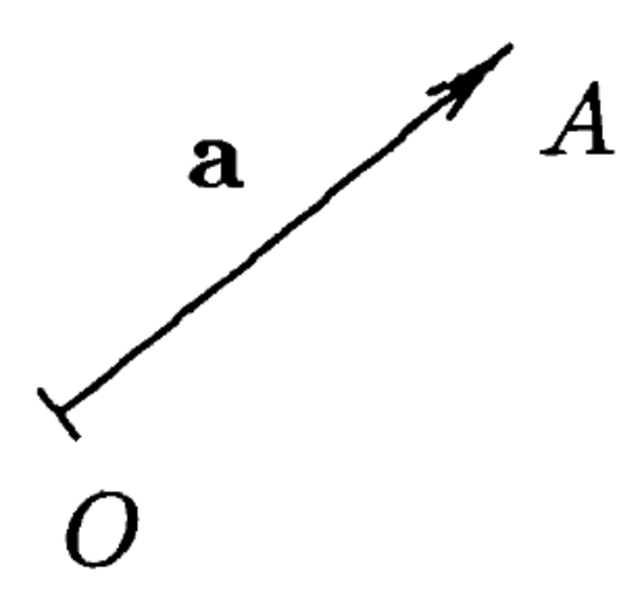
\includegraphics[width=0.5\linewidth]{figures/vector.pdf}
			\end{center}\vspace{-0.7cm}
			\caption{Vetor\label{fig:vector} \cite{lounestoClifford}.}
		\end{figure}
	\end{minipage}
	
	Assim, um vetor $\mathbf a$ e seu oposto $-\mathbf a$ tem o mesmo comprimento e direção, mas possuem sentidos opostos. Também, dois vetores são iguais se, e somente se, possuem a mesma magnitude, direção e sentido. Isso é, para $\mathbf{a}$ e $\mathbf{b}$ vetores,
	$$\mathbf a = \mathbf b \iff \norm{\mathbf{a}} = \norm{\mathbf{b}} \text{ e } \mathbf{a}\upuparrows\mathbf{b}.$$
	Aqui introduz-se a notação de mesma direção e sentido como $\upuparrows$, absorvida de \cite{lounestoClifford}, donde retirou-se vários dos resultados aqui mostrados. Escreveremos $\updownarrows$ quando as direções forem iguais, mas o sentido oposto.
	
	Quando se trata da operação do espaço vetorial (a adição) também temos uma interpretação geométrica. Dados dois vetores $\mathbf a$ e $\mathbf b$, desenha-se um paralelogramo com lados formados por estes vetores (conforme Figura~\ref{fig:paralelogram}) e a diagonal deste paralelogramo será a soma de $\mathbf a$ com $\mathbf b$. Perceba que a interpretação respeita a comutatividade e que compreende a subtração, dada a soma pelo oposto.
	
	\begin{figure}[H]
		\begin{center}
			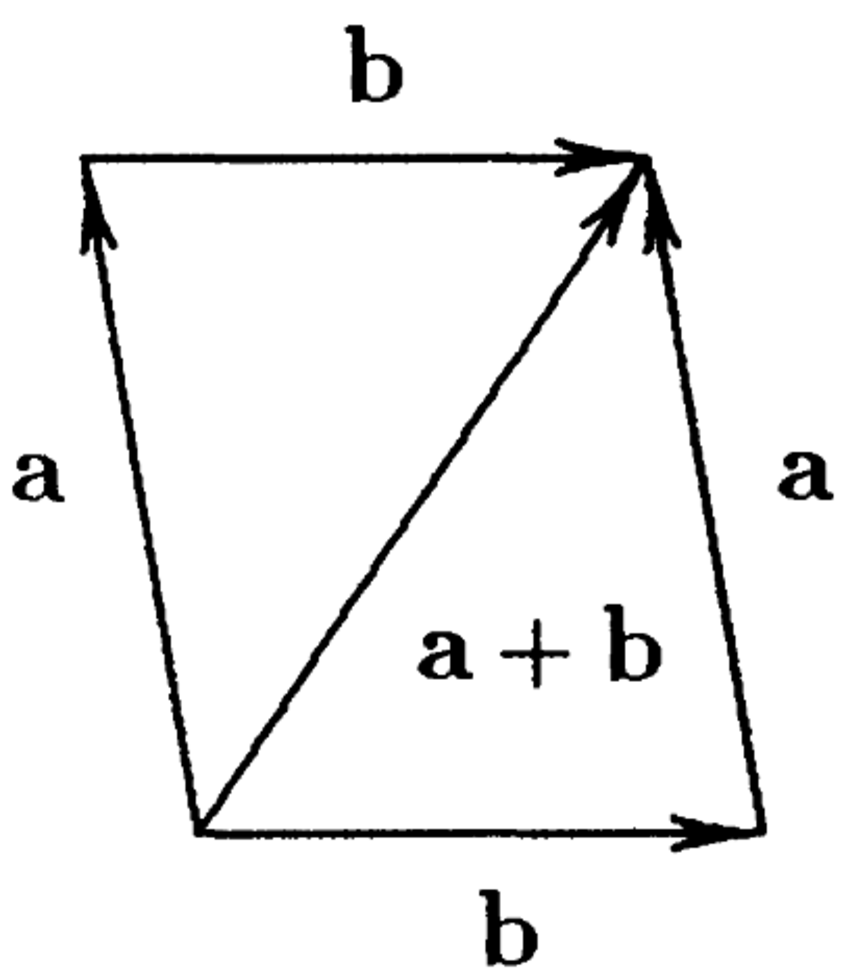
\includegraphics[width=0.22\linewidth]{figures/paralelogram.pdf}
		\end{center}
		\caption{Interpretação geométrica da soma de vetores \cite{lounestoClifford}.}
		\label{fig:paralelogram}
	\end{figure}
	
	Podemos tecer uma interpretação geométrica da multiplicação por escalar associada a um espaço vetorial. Se $\lambda\in K$ é um escalar de um espaço vetorial $E$ sobre $K$, então o vetor $\mathbf a$ pode ser ``esticado'' por um escalar $\lambda$ (se $\lambda>1$) ou ``comprimido'' (se $0<\lambda<1$). Também, se $\lambda<0$, então $\lambda \mathbf a$ terá sentido contrário ao de $\mathbf a$. Isso é fácil de compreender visto a associatividade do produto por escalar $(-\lambda)\mathbf a = \lambda(-\mathbf a).$
	
	
	\begin{minipage}{0.3\linewidth}
		Assim, temos que $$\lambda \mathbf a \upuparrows \mathbf a, \text{ se } \lambda > 0,$$ $$\lambda \mathbf a \updownarrows \mathbf a, \text{ se } \lambda < 0.$$
	\end{minipage}
	\begin{minipage}{0.7\linewidth}
		\begin{figure}[H]
			\begin{center}
				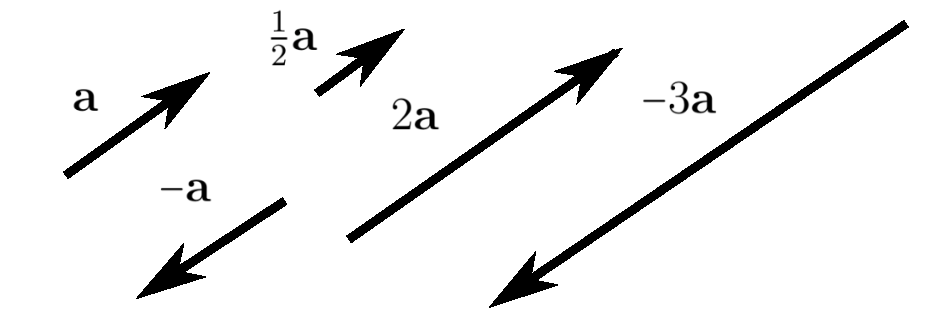
\includegraphics[width=0.7\linewidth]{figures/scalarProduct.pdf}
			\end{center}
			\caption{Produto por escalar.}
			\label{fig:scalarProduct}
		\end{figure}
	\end{minipage}
	\\
	
	Por fim, também temos uma interpretação para um produto entre dois vetores, que chamamos de produto escalar. Essa operação associa dois elementos $\mathbf a, \mathbf b$ no espaço vetorial $E$ sobre $K$ com um elemento do corpo $K$ que é proporcional ao produto dos módulos de $\mathbf a$ e $\mathbf b$ e o cosseno do ângulo $\varphi$ entre estes dois vetores. Ou seja, $$\mathbf a \cdot \mathbf b = \norm{\mathbf a}\norm{\mathbf b}\cos \varphi,\quad \text{ com } 0\leq\varphi\leq 180^\circ.$$
	Dessa forma, se o ângulo entre os vetores é 90$^\circ$ (i.e., são perpendiculares), $\mathbf a \cdot \mathbf b = 0$.\\
	
	Com isso, estamos familiarizados com as noções de soma entre vetores (consequentemente com subtração), soma e multiplicação entre escalares (que, como são elementos de um corpo, subentendem subtração e divisão), com a de multiplicação de um vetor por um escalar (resultando em vetor) e com a noção de multiplicação entre vetores (resultando em escalar). É intuitivo se perguntar se é possível multiplicar dois vetores e obter um vetor. De fato, existe um produto do tipo em Álgebra Linear, chamado de produto vetorial, mas ele é apenas definido sobre o $\mathbb{R}^3$. Agora iremos introduzir um produto entre vetores mais geral (chamado \textit{produto exterior}) mas, para isso, primeiro precisaremos abordar a natureza do elemento que ele resultará.
	
	\subsubsection{Bivetores}
	
	Seja $\mathbf A$ uma área de superfície plana em um plano $P$, dotada de um ``sentido'' (representado por uma flecha de rotação, assim como na Figura~\ref{fig:2blade}). Se $\mathbf A'$ representa outra área de superfície plana em outro plano $P'$, também dotada de um sentido, então pode-se definir a seguinte relação de equivalência: $\mathbf A$ é equivalente a $\mathbf A'$ se, e somente se, $P$ e $P'$ são paralelos, as áreas de $\mathbf A$ e $\mathbf A'$ são iguais e se os seus sentidos (de rotação) são o mesmo depois de transladar $\mathbf A'$ em $\mathbf A$ (ou seja, $P'$ para $P$). As classes de equivalência formadas por essas áreas orientadas de superfície plana são chamadas de \textit{$2$-vetor} (ou, um \textit{bivetor}).

	\begin{figure}[H]
		\begin{center}
			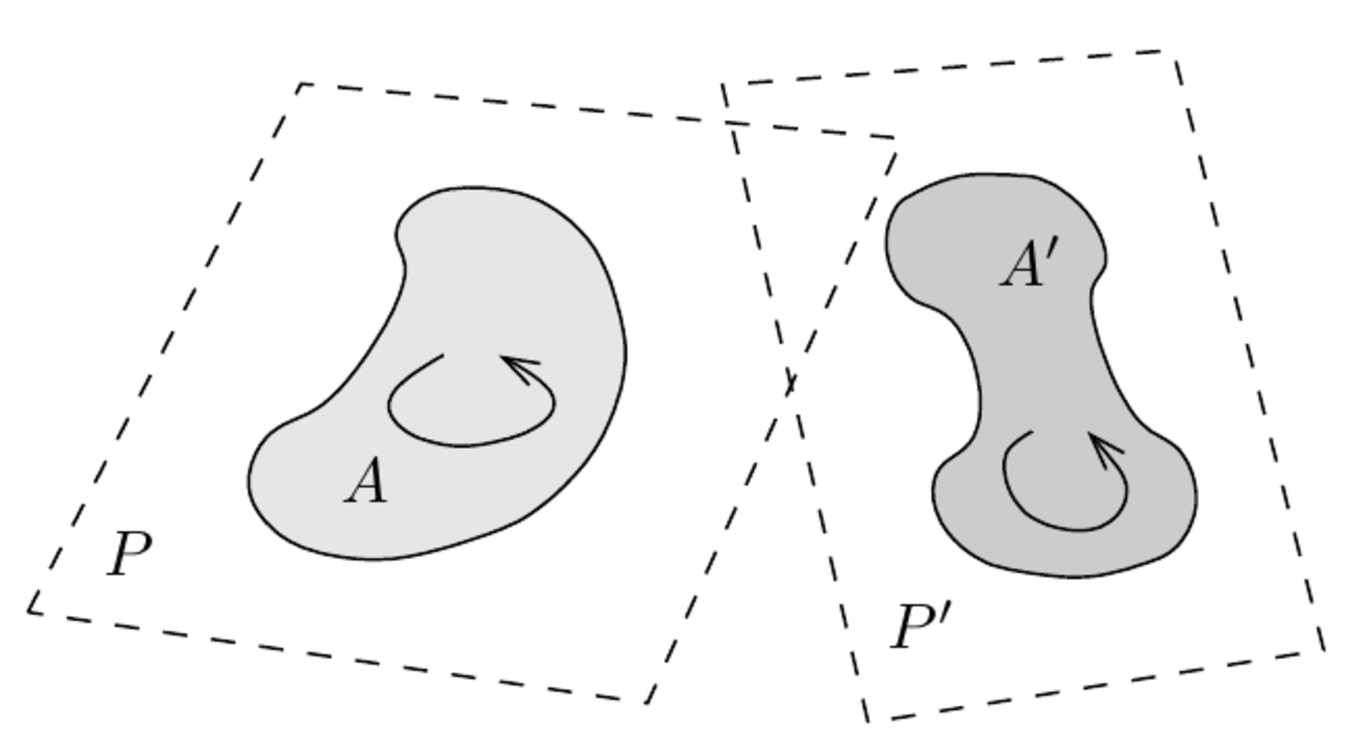
\includegraphics[width=0.5\linewidth]{figures/2blade.pdf}
		\end{center}
		\caption{Áreas de superfícies planas $\mathbf A$ e $\mathbf A'$ nos respectivos planos $P$ e $P'$ \cite{lundholm2009clifford}.}
		\label{fig:2blade}
	\end{figure}
	
	Perceba que o bivetor $\mathbf A$ (de qualquer formato) pode ser representado por um paralelogramo de lados $\mathbf a$ e $\mathbf b$ tais que a área orientada de superfície plana assim formada seja equivalente a $\mathbf A$ (vide Figura~\ref{fig:2bladePlano}). A esse quadrilátero chamamos de \textit{produto exterior de $\mathbf a$ com $\mathbf b$} e escrevemos $\mathbf a \wedge \mathbf b$. Se a área de $\mathbf A$ é zero, então escrevemos $\mathbf A = 0$. Assim, $\mathbf a \wedge \mathbf a = 0$. Também, por $-\mathbf A$ expressamos a classe de equivalência de todas as áreas orientadas de superfície plana com a mesma área e no mesmo plano que $\mathbf A$, mas com um sentido de rotação contrário ao de $\mathbf A$. Perceba que $-(\mathbf a \wedge \mathbf b) = \mathbf b \wedge \mathbf a$ (Figura~\ref{fig:2bladePlano}). Um \textit{bivetor unidade} é um bivetor $\mathbf A$ com $\norm{\mathbf A} = 1$.
	
	\begin{figure}[H]
		\begin{center}
			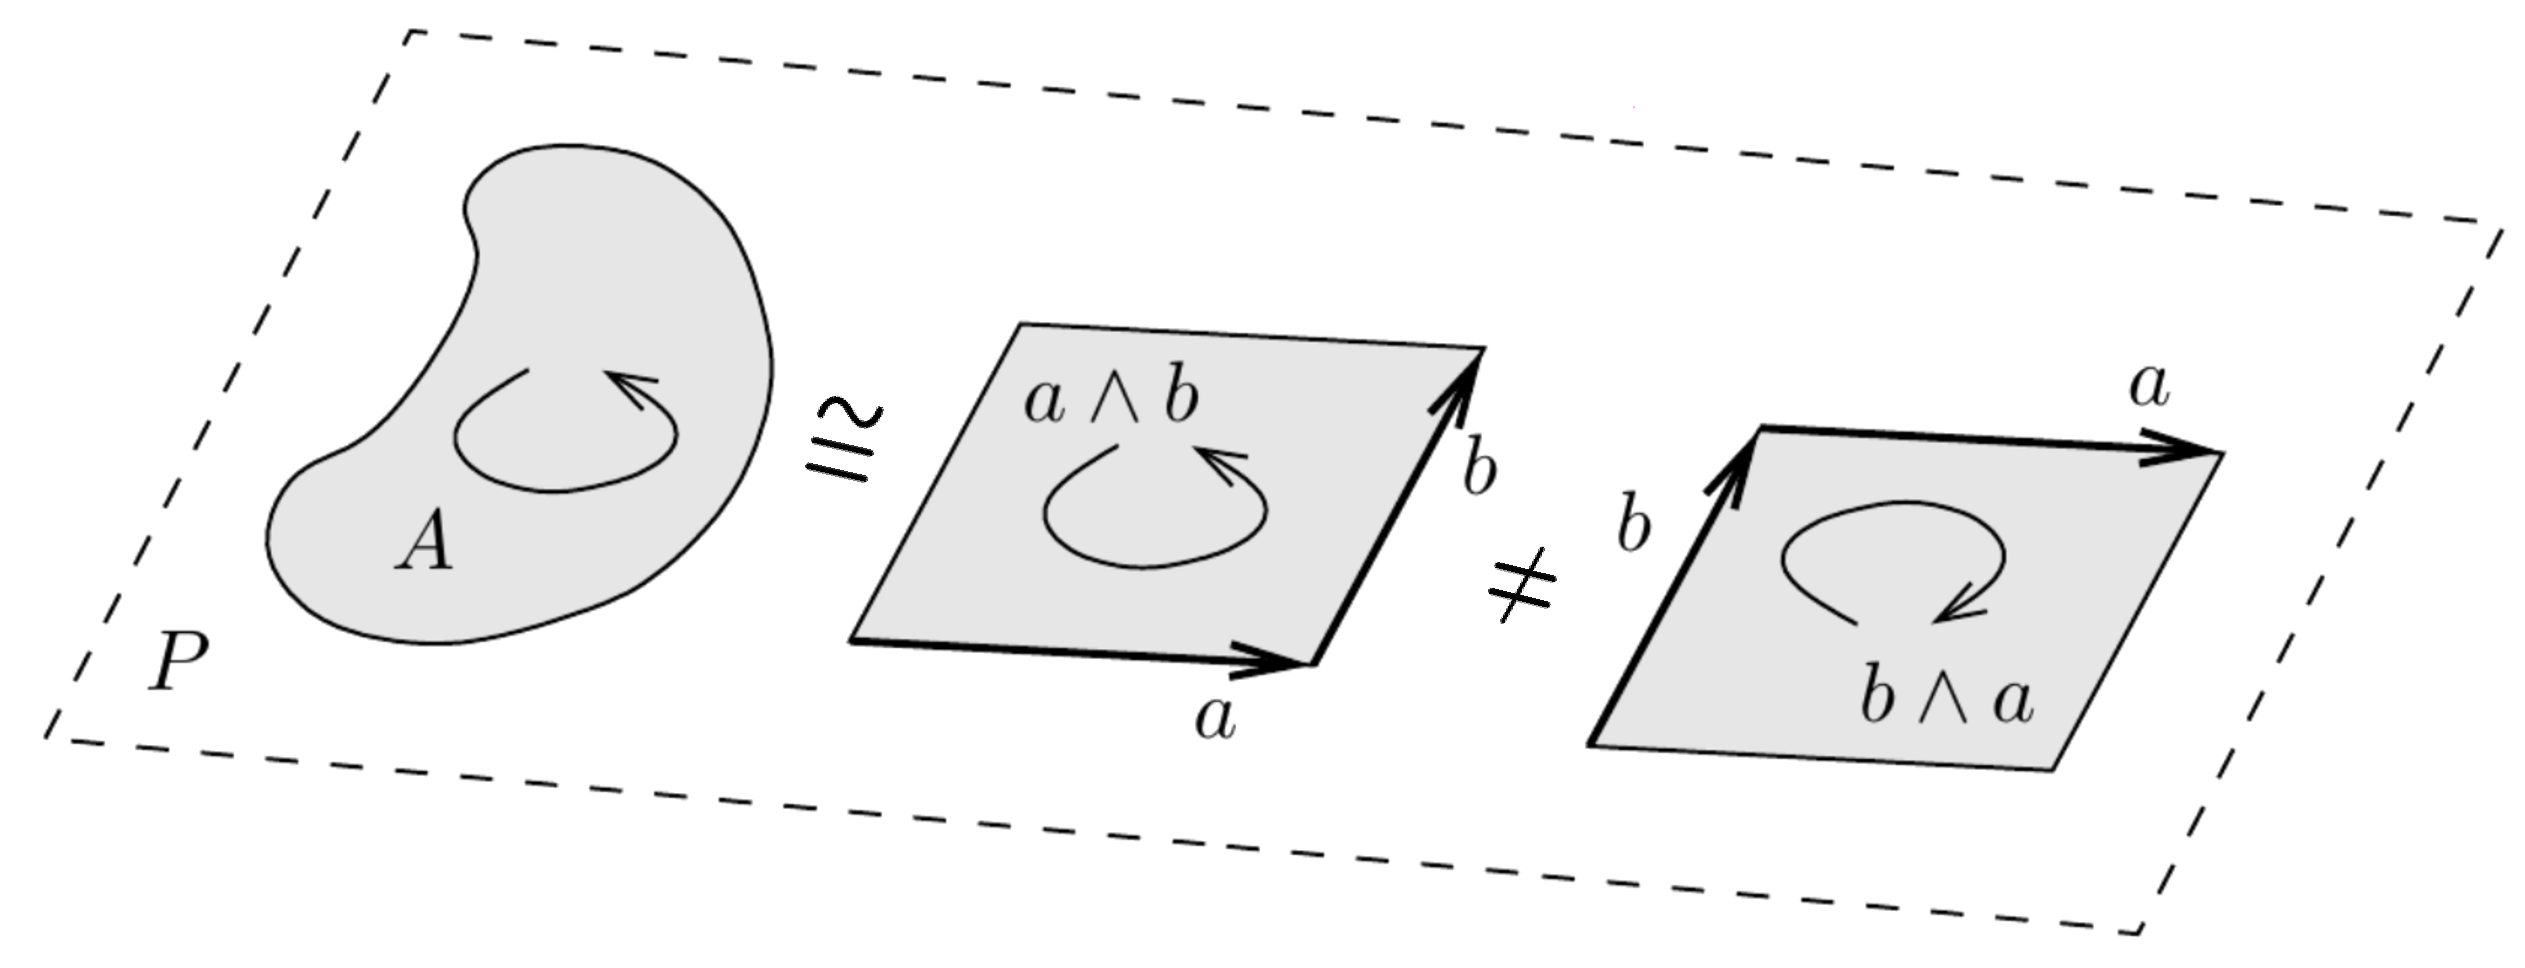
\includegraphics[width=0.75\linewidth]{figures/2bladePlano.pdf}
		\end{center}
		\caption{Um bivetor representado por um produto exterior $\mathbf a\wedge \mathbf b$ e $\mathbf b \wedge \mathbf a$ \cite{lundholm2009clifford}.}
		\label{fig:2bladePlano}
	\end{figure}
	
	\subsubsection{Adição de bivetores}
	
	A interpretação geométrica da adição de bivetores pode ser facilmente vista se existir um vetor comum entre os bivetores e, por sorte, em três dimensões sempre existe ao menos uma reta que intercepta dois planos quaisquer. Dessa forma, sejam $\mathbf A = \mathbf a \wedge \mathbf c$ e $\mathbf B = \mathbf b \wedge \mathbf c$ dois bivetores, então o bivetor $\mathbf A + \mathbf B$ é definido por $$\mathbf A+\mathbf B = \mathbf a \wedge \mathbf c + \mathbf b \wedge \mathbf c = (\mathbf a+ \mathbf b) \wedge \mathbf c.$$ 
	
	\begin{figure}[H]
		\begin{center}
			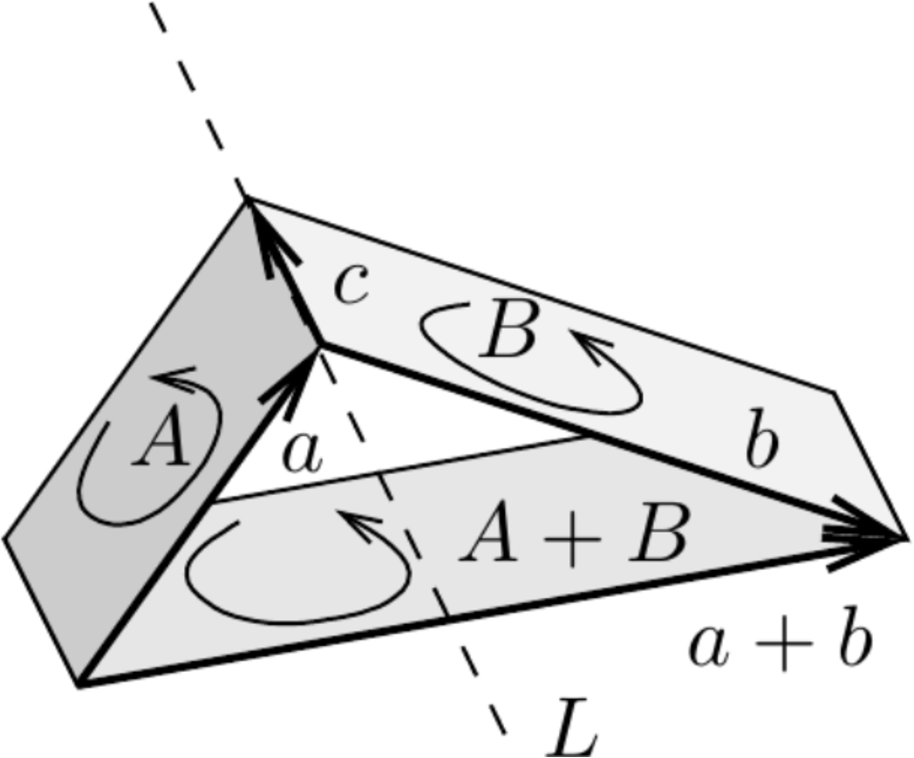
\includegraphics[width=0.32\linewidth]{figures/2bladeSoma.pdf}
		\end{center}
		\caption{Interpretação geométrica da soma $\mathbf A+\mathbf B = (\mathbf a+\mathbf b)\wedge c$ \cite{lundholm2009clifford}.}
		\label{fig:2bladeSoma}
	\end{figure}
	
	Perceba que, como a soma de vetores é comutativa, $\mathbf A+\mathbf B = \mathbf B+\mathbf A$ e, portanto, o conjunto de bivetores sobre a adição forma um grupo abeliano. Bivetores também podem ser operados com escalares do corpo dos reais, donde eles se tornam um espaço vetorial. Descrevemos esse espaço por $\bigwedge^2\mathbb{R}^3$. Uma base para esse espaço vetorial pode ser construída usando a base $\{\mathbf e_1,\mathbf e_2,\mathbf e_3\}$ do espaço vetorial $\mathbb{R}^3$. As áreas orientadas de superfície plana obtidas através dos produtos exteriores $\mathbf e_1 \wedge \mathbf e_2, \mathbf e_3 \wedge \mathbf e_1, \mathbf e_2 \wedge \mathbf e_3$, entre os elementos da base de $\mathbb{R}^3$, formam uma base para o espaço vetorial $\bigwedge^2\mathbb{R}^3$.
	
	\begin{minipage}{0.35\linewidth}
		\vspace{-0.5cm}
		\begin{figure}[H]
			\begin{center}
				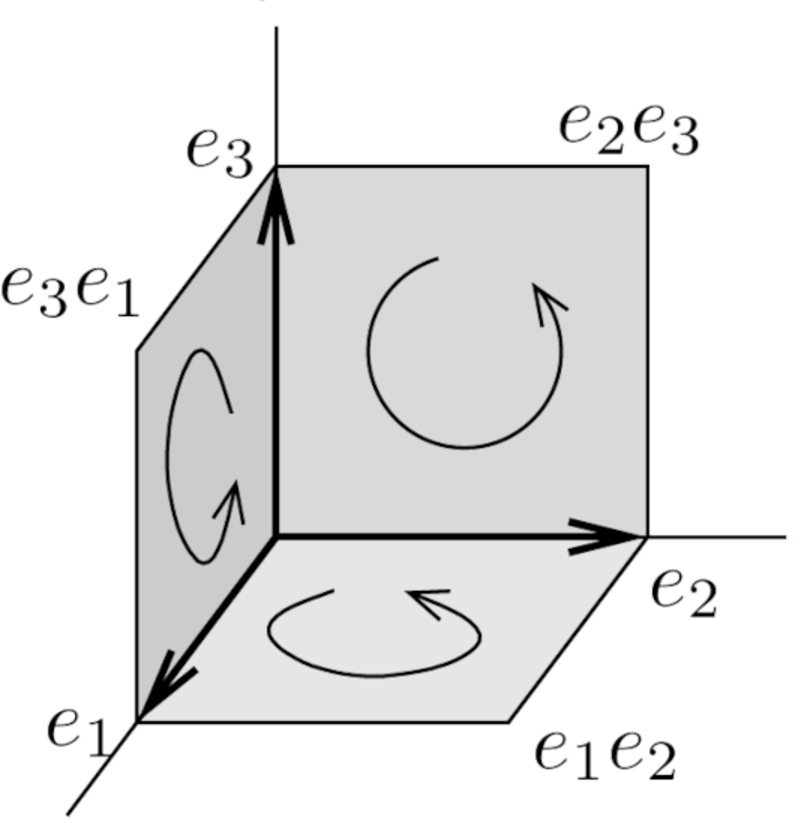
\includegraphics[width=0.7\linewidth]{figures/bivectorsBase.pdf}
			\end{center}\vspace{-0.7cm}
			\caption{Base do $\bigwedge^2\mathbb{R}^3$ \cite{lounestoClifford}.}
			\label{fig:bivectorsBase}
		\end{figure}
	\end{minipage}
	\begin{minipage}{0.6\linewidth}%\vspace{0.5cm}
		\setlength\parindent{24pt} Assim, um bivetor arbitrário $\mathbf B$ é uma combinação linear dos elementos da base: $$\mathbf B = B_{1,2}\mathbf e_1\wedge \mathbf e_2 + B_{3,1}\mathbf e_3\wedge \mathbf e_1 + B_{2,3}\mathbf e_2\wedge \mathbf e_3.$$ O produto escalar do $\mathbb{R}^3$ é estendido para um produto simétrico bilinear no espaço dos bivetores $\bigwedge^2\mathbb{R}^3$, da forma $$<\mathbf x_1\wedge \mathbf x_2, \mathbf y_1\wedge\mathbf y_2> \,=
		\begin{tabular}{| c c |}
			$\mathbf x_1\cdot \mathbf y_1$ & $\mathbf x_1\cdot \mathbf y_2$\\
			$\mathbf x_2\cdot \mathbf y_1$ & $\mathbf x_2\cdot \mathbf y_2$\\
		\end{tabular}.
		$$
	\end{minipage}
	Em particular, $<\mathbf a\wedge \mathbf b, \mathbf a\wedge\mathbf b>\, = \norm{\mathbf a}^2\norm{\mathbf b}^2 - (\mathbf a \cdot \mathbf b)^2$. Pode-se definir a norma (ou área) de $\mathbf B$ como $$\norm{ \mathbf B} = \sqrt{B_{1,2}^2 + B_{3,1}^2 + B_{2,3}^2}.$$
	
	Nesse momento podemos traçar uma relação entre o produto vetorial estudado em Álgebra Linear e o produto exterior de Grassmann. Sejam $\mathbf a = a_1\mathbf e_1+a_2\mathbf e_2 + a_3\mathbf e_3$ e $\mathbf b = b_1\mathbf e_1 + b_2\mathbf e_2 + b_3\mathbf e_3$ vetores. O bivetor $$\mathbf a \wedge\mathbf b = (a_2b_3 - a_3b_2)\mathbf e_2\wedge\mathbf e_3 + (a_3b_1 - a_1b_3)\mathbf e_3 \wedge\mathbf e_1 + (a_1b_2 - a_2b_1)\mathbf e_1\wedge\mathbf e_2$$ pode ser expresso como um ``determinante'' $$\mathbf a \wedge \mathbf b = 
	\begin{tabular}{| c c c |}
		$\mathbf e_2 \wedge \mathbf e_3$& $\mathbf e_3 \wedge \mathbf e_1$& $\mathbf e_1 \wedge \mathbf e_2$\\
		$a_1$ &$a_2 $&$a_3 $\\
		$b_1 $&$b_2$ &$b_3 $
	\end{tabular}.$$ E relembrando, define-se o \textit{produto vetorial de $\mathbf a$ por $\mathbf b$} como $$\mathbf a\times \mathbf b = (a_2b_3 - a_3b_2)\mathbf e_1 + (a_3b_1 - a_1b_3)\mathbf e_2+ (a_1b_2 - a_2b_1)\mathbf e_3,$$ que, por sua vez, pode ser representado pelo ``determinante'' $$\mathbf a \times \mathbf b = 
	\begin{tabular}{| c c c |}
		$\mathbf e_1$& $\mathbf e_2$& $\mathbf e_3$\\
		$a_1$ &$a_2 $&$a_3 $\\
		$b_1 $&$b_2$ &$b_3 $
	\end{tabular}.$$
	
	A interpretação geométrica de $\mathbf a\times \mathbf b$ é um vetor perpendicular ao plano de $\mathbf a\wedge\mathbf b$ e com norma igual a área do paralelogramo formado por $\mathbf a$ e $\mathbf b$, isso é, $$\norm{\mathbf a\times\mathbf b} = \norm{\mathbf a \wedge \mathbf b} = \norm{\mathbf a}\norm{\mathbf b}\sin\varphi,$$ onde $0\leq\varphi\leq180^\circ$ é o ângulo entre $\mathbf a$ e $\mathbf b$.
	
	\begin{figure}[H]
		\begin{center}
			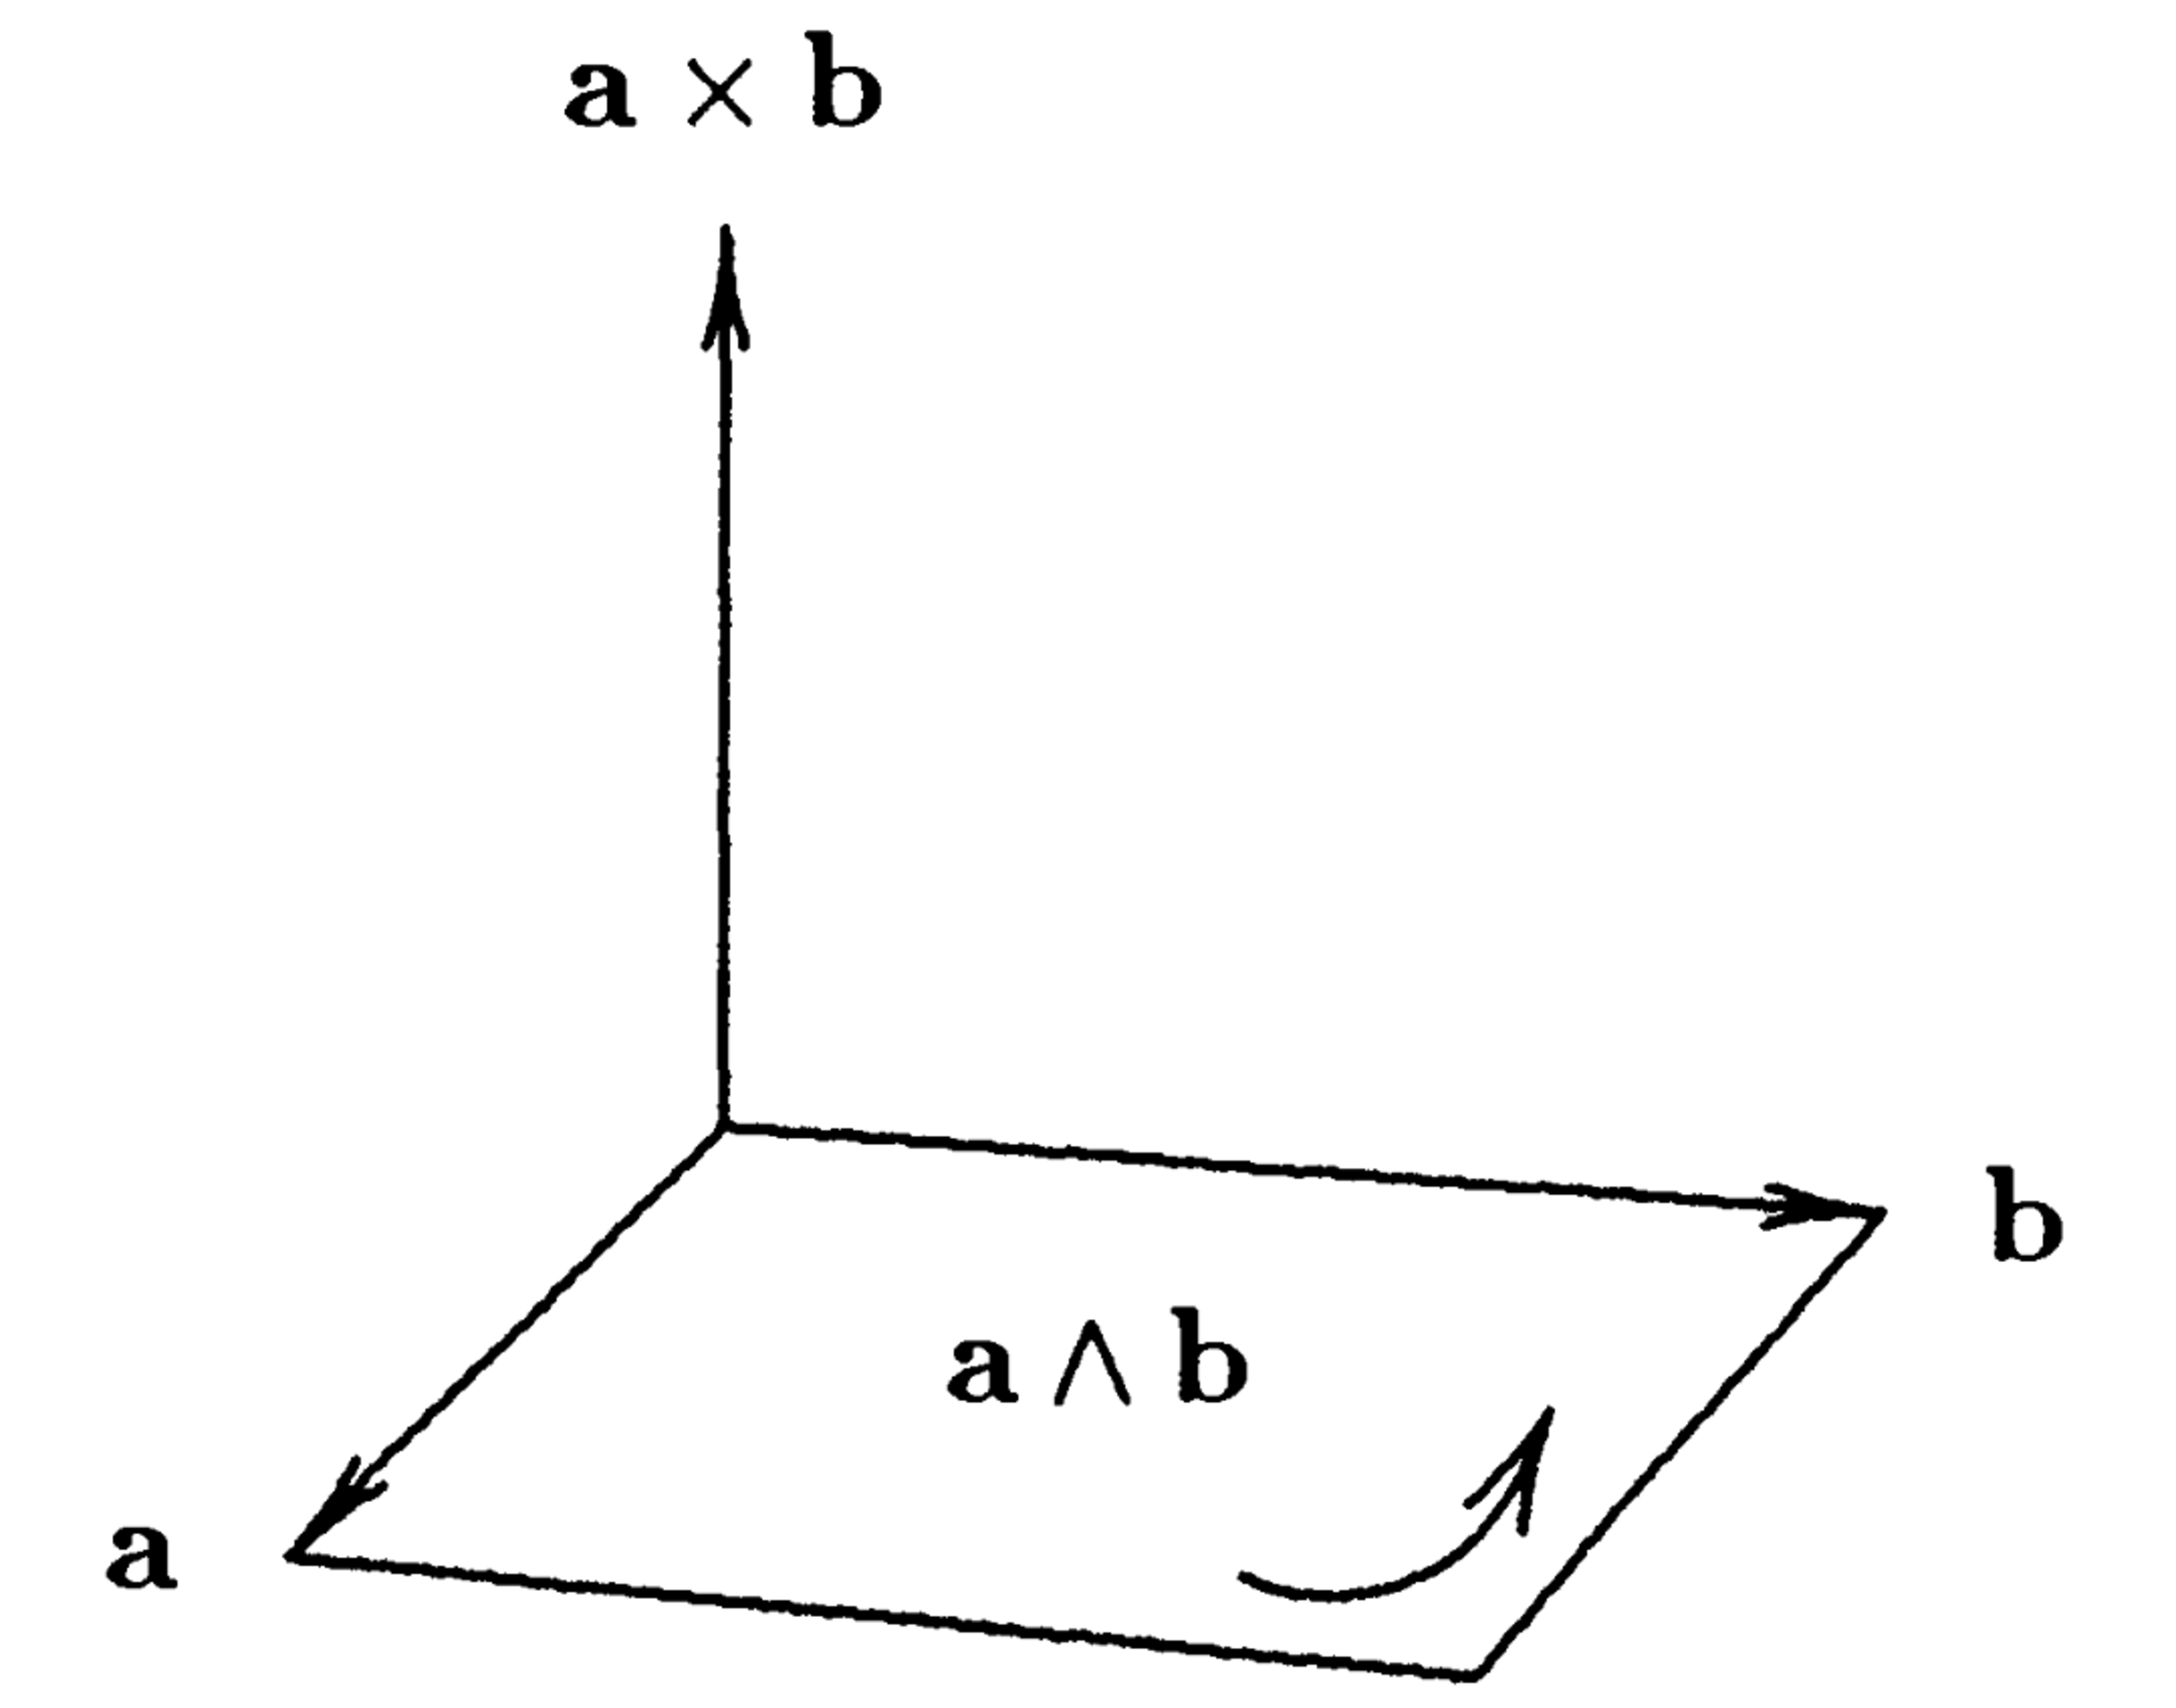
\includegraphics[width=0.35\linewidth]{figures/produtoVetorial.pdf}
		\end{center}
		\caption{Interpretação geométrica de $\mathbf a \times \mathbf b$ \cite{lounestoClifford}.}
		\label{fig:produtoVetorial}
	\end{figure}
	
	\subsubsection{Trivetores}
	O produto exterior $\mathbf a \wedge\mathbf b\wedge\mathbf c$ de três vetores $\mathbf a = a_1\mathbf e_1+a_2\mathbf e_2+a_3\mathbf e_3$, $\mathbf b = b_1\mathbf e_1+b_2\mathbf e_2+b_3\mathbf e_3$ e $\mathbf c = c_1\mathbf e_1+c_2\mathbf e_2+c_3\mathbf e_3$ representa o volume orientado do paralelepípedo com lados $\mathbf a$, $\mathbf b$ e $\mathbf c$: $$\mathbf a\wedge\mathbf b\wedge\mathbf c = \begin{tabular}{|c c c|}
		$a_1$&$a_2$&$a_3$\\
		$b_1$&$b_2$&$b_3$\\
		$c_1$&$c_2$&$c_3$
	\end{tabular}
	\ \mathbf e_1\wedge\mathbf e_2\wedge\mathbf e_3.
	$$
	Esse é um elemento do espaço vetorial unidimensional de trivetores (ou, 3-vetores) $\bigwedge^3\mathbb{R}^3$, com base $\mathbf e_1\wedge\mathbf e_2\wedge\mathbf e_3$. O produto exterior é associativo, isso é, $$(\mathbf a\wedge \mathbf b)\wedge \mathbf c = \mathbf a\wedge (\mathbf b\wedge \mathbf c),$$ e antissimétrica: $$\mathbf a \wedge \mathbf b \wedge \mathbf c = \mathbf b \wedge \mathbf c \wedge \mathbf a = \mathbf c \wedge \mathbf a \wedge \mathbf b = -\mathbf c \wedge \mathbf b \wedge \mathbf a = - \mathbf a \wedge \mathbf c \wedge \mathbf b = -\mathbf b \wedge \mathbf a \wedge \mathbf c, \quad \forall \mathbf a, \mathbf b, \mathbf c\in \mathbb{R}^3$$
	
	O produto exterior dos elementos da base $\mathbf e_1,\mathbf e_2,\mathbf e_3$ do $\mathbb{R}^3$ é o volume orientado unitário $\mathbf e_1 \wedge\mathbf e_2 \wedge\mathbf e_3 \in \bigwedge^3\mathbb{R}^3$. O volume (ou norma) $\norm{\mathbf V}$ de um trivetor $\mathbf V = V\mathbf e_1\wedge\mathbf e_2\wedge\mathbf e_3$ é $\norm{V}$, isso é, $\norm{V\mathbf e_1\wedge\mathbf e_2\wedge\mathbf e_3} = V$ para $V\geq 0$ e $\norm{V\mathbf e_1\wedge\mathbf e_2\wedge\mathbf e_3} = -V$ para $V<0$.
	
	\subsubsection{O dual de Hodge}
	
	Como tanto o espaço vetorial do $\mathbb{R}^3$ quanto o $\bigwedge^2\mathbb{R}^3$ possuem dimensão finita igual a 3 e ambos são definidos sobre o corpo dos reais $\mathbb{R}$, então eles são isomorfos. Pode-se usar a métrica sobre o espaço vetorial $\mathbb{R}^3$ para gerar um isomorfismo entre estes espaços vetoriais. O dual de Hodge relaciona um vetor $\mathbf a \in \mathbb{R}^3$ a um bivetor $*\mathbf a \in \bigwedge^2\mathbb{R}^3$, através de $$\mathbf b \wedge*\mathbf a = (\mathbf b \cdot \mathbf a)\mathbf e_1\wedge \mathbf e_2 \wedge\mathbf e_3, \quad \text{ para todo } \mathbf b\in \mathbb{R}^3.$$
	
	O dual de Hodge depende não apenas da métrica (induzida pelo produto interno) mas também da escolha da orientação. Costuma-se usar a mão direita e a base ortonormal $\{\mathbf e_1,\mathbf e_2,\mathbf e_3\}$.
	
	\begin{figure}[H]
		\begin{center}
			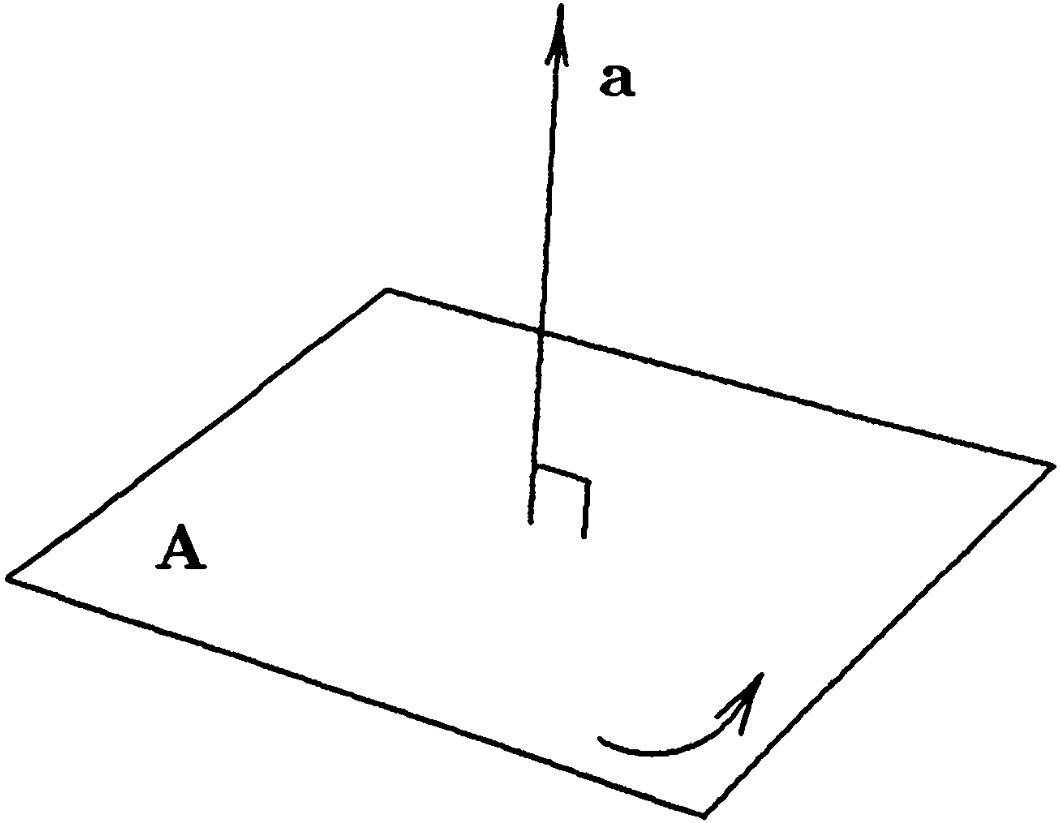
\includegraphics[width=0.4\linewidth]{figures/dual.jpg}
		\end{center}
		\caption{O vetor $\mathbf a$ e seu dual $\mathbf A = \mathbf a\mathbf e_{123}$}
		\label{fig:lable}
	\end{figure}
	
	Assim, associamos a cada vetor $$\mathbf a = a_1\mathbf e_1+a_2\mathbf e_2 + a_3 \mathbf e_3\ \in \mathbb{R}^3$$ um bivetor $$\mathbf A = *\mathbf a = a_1\mathbf e_2\wedge\mathbf e_3 + a_2 \mathbf e_3\wedge\mathbf e_1 + a_3 \mathbf e_1\wedge\mathbf e_2\ \in \bigwedge^2\mathbb{R}^3.$$
	
	Usando a métrica induzida sobre o espaço de bivetores $\bigwedge^2\mathbb{R}^3$, pode-se estender o dual de Hodge para um mapeamento que associa um bivetor $\mathbf A\in \bigwedge^2\mathbb{R}^3$ com um vetor $*\mathbf A\in \mathbb{R}^3$, definido por $$\mathbf B \wedge*\mathbf A =\, <\mathbf B, \mathbf A>\mathbf e_1\wedge \mathbf e_2 \wedge\mathbf e_3, \quad \text{ para todo } \mathbf B\in \bigwedge^2\mathbb{R}^3.$$
	
	Usando esta dualidade, pode-se escrever a relação entre o produto externo e o produto vetorial como $$\mathbf a\wedge\mathbf b = *(\mathbf a\times \mathbf b), \quad \text{ e }\quad \mathbf a\times \mathbf b = *(\mathbf a\wedge\mathbf b).$$
	 
	\subsection{Álgebra Exterior $\bigwedge\mathbb{R}^3$}
	
	A álgebra exterior $\bigwedge\mathbb{R}^3$ do espaço vetorial $\mathbb{R}^3$ foi construída por Grassmann em 1844, em sua Teoria da Expansão \cite{grassmannLineale}, e é uma soma direta dos subespaços de escalares ($\mathbb{R}$, com base $\{1\}$), de vetores ($\mathbb{R}^3$, com base $\{\mathbf e_1,\mathbf e_2,\mathbf e_3\}$), de bivetores ($\bigwedge^2\mathbb{R}^3$, com base $\{\mathbf e_1\wedge\mathbf e_2, \mathbf e_2\wedge\mathbf e_3, \mathbf e_3\wedge\mathbf e_1\}$) e de trivetores ($\bigwedge^3\mathbb{R}^3$, com base $\{\mathbf e_1\wedge\mathbf e_2\wedge\mathbf e_3\}$). Podemos reescrever $\mathbb{R} = \bigwedge^0\mathbb{R}^3$ e $\mathbb{R}^3 = \bigwedge^1\mathbb{R}^3$ e, assim, escrevemos a álgebra exterior como $$\bigwedge\mathbb{R}^3 = \bigwedge^0\mathbb{R}^3 \oplus \bigwedge^1\mathbb{R}^3\oplus \bigwedge^2\mathbb{R}^3 \oplus \bigwedge^3\mathbb{R}^3.$$
	Como as respectivas dimensões de $\mathbb{R}, \mathbb{R}^3, \bigwedge^2\mathbb{R}^3$ e $\bigwedge^3\mathbb{R}^3$ são $1,3,3,1$, a dimensão de $\bigwedge\mathbb{R}^3$ é 8.
	 
	A álgebra exterior $\bigwedge\mathbb{R}^3$ é uma álgebra associativa com unidade $1$ e satisfazendo $$\mathbf e_i\wedge\mathbf e_i = 0\quad \text{ e } \quad\mathbf e_i\wedge\mathbf e_j = -\mathbf e_j \wedge\mathbf e_i, \text{ para } i\neq j$$ para a base $\{\mathbf e_1,\mathbf e_2,\mathbf e_3\}$ do espaço vetorial $\mathbb{R}^3$. O produto exterior de dois elementos homogêneos satisfaz
	$$\mathbf a\wedge\mathbf b\in \bigwedge^{i+j}\mathbb{R}^3\text{ para } \mathbf a\in \bigwedge^i\mathbb{R}^3, \mathbf b\in \bigwedge^j\mathbb{R}^3.$$	
	
	\subsection{Álgebra Geométrica $\mathcal C \ell_3$}
	A álgebra exterior $\bigwedge\mathbb{R}^3$ contém uma cópia do $\mathbb{R}^3$, o que permite a aplicações de diversos cálculos para a geometria do $\mathbb{R}^3$. Porém, um inconveniente que aparece quando se trabalha com $\bigwedge\mathbb{R}^3$ é que o produto nessa álgebra não preserva a norma, isso é, $\norm{\mathbf a\wedge\mathbf b} = \norm{\mathbf a}\norm{\mathbf b}\sin\varphi \leq \norm{\mathbf a}\norm{\mathbf b}$. Encontrar um novo produto entre vetores de forma que se preservasse a igualdade $\norm{\text{``}\mathbf a\mathbf b\text{''}} = \norm{\mathbf a}\norm{\mathbf b}$ possibilitaria, por exemplo, a representação de rotações como operações nesta álgebra \cite{lounestoClifford}. 
	
	\subsubsection{O produto de Clifford}
	
	Um novo tipo de produto entre vetores, chamado \emph{produto de Clifford dos vetores $\mathbf a$ e $\mathbf b$} é obtido pela adição do escalar $\mathbf a\cdot \mathbf b$ e do bivetor $\mathbf a\wedge\mathbf b$: $$\mathbf a\mathbf b = \mathbf a\cdot \mathbf b + \mathbf a\wedge \mathbf b.$$
	
	Estamos unindo um produto comutativo com um anticomutativo. Por conta disso, temos que $$\mathbf b\mathbf a = \mathbf a\cdot \mathbf b - \mathbf a\wedge\mathbf b,$$
	o que implica que $\mathbf a\cdot \mathbf b = \dfrac 1 2 (\mathbf a\mathbf b + \mathbf b\mathbf a)$ e $\mathbf a\wedge \mathbf b = \dfrac 1 2 (\mathbf a\mathbf b - \mathbf b\mathbf a)$.
	\\
	
	Como o produto interno e o exterior zeram quando os vetores são, respectivamente, perpendiculares e paralelos, segue que dois vetores $\mathbf a$ e $\mathbf b$ são paralelos se seu produto comuta, isso é, $\mathbf a \mathbf b = \mathbf b \mathbf a$ e são perpendiculares quando seu produto anticomuta, isso é, $\mathbf a\mathbf b = -\mathbf b\mathbf a$.
	\\
	
	Pode-se calcular o produto $\mathbf a\mathbf b\mathbf b\mathbf a$ para obter que $\mathbf a^2\mathbf b^2 = (\mathbf a\cdot \mathbf b)^2 - (\mathbf a\wedge \mathbf b)^2$ e usar que $(\mathbf a\wedge\mathbf b)^2 = -\norm{\mathbf a\wedge\mathbf b}^2$ para obter a identidade
	$$\mathbf a^2\mathbf b^2 = (\mathbf a\cdot\mathbf b)^2 + \norm{\mathbf a\wedge\mathbf b}^2$$
	que implica que $(\mathbf a\mathbf b)^2 = (\norm{\mathbf a}\norm{\mathbf b}\cos\varphi)^2 + (\norm{\mathbf a}\norm{\mathbf b}\sin\varphi)^2 = \norm{\mathbf a}^2\norm{\mathbf b}^2$, isso é, se e somente se $$\norm{\mathbf a\mathbf b} = \norm{\mathbf a}\norm{\mathbf b}.$$
	
	\subsubsection{Base de $\mathcal C \ell_3$}
	
	Assim, através desse novo produto, definimos uma base para a chamada Álgebra Geométrica $\mathcal C \ell_3$ do espaço Euclidiano $\mathbb{R}^3$. A base $\{\mathbf e_1,\mathbf e_2,\mathbf e_3\}$ da cópia do espaço vetorial $\mathbb{R}^3$ dentro de $\mathcal C \ell_3$ satisfará as seguintes propriedades
	$$\mathbf e_i\mathbf e_j = -\mathbf e_j\mathbf e_i, \text{ para } i\neq j\quad\text{ e }\quad \mathbf e_i\mathbf e_i = 1,$$
	que dizem respeito respectivamente a ortogonalidade entre diferentes elementos da base e ao paralelismo entre dois vetores iguais. Clifford inventou essas novas regras partindo da álgebra exterior em 1882, buscando uma álgebra associativa que mantivesse $\mathbf e_i\mathbf e_j = \mathbf e_i\wedge\mathbf e_j$ e, inicialmente, em 1878, propôs um produto que levava $\mathbf e_i\mathbf e_i = -1$.
	
	Pode-se associar a base do espaço vetorial de $\mathcal C \ell_3$ com a base de $\bigwedge\mathbb{R}^3$ pois, da mesma forma que em $\bigwedge\mathbb{R}^3$, construímos a Álgebra Geométrica $\mathcal C \ell_3$ como as somas diretas $$\mathcal C \ell_3 = \mathbb{R} \oplus \mathbb{R}^3\oplus \bigwedge^2\mathbb{R}^3 \oplus \bigwedge^3\mathbb{R}^3.$$
	
	Essa separação em bases induz uma estrutura de multivetor na Álgebra Geométrica $\mathcal C \ell_3$. Essa estrutura de multivetor é única, isso é, um elemento arbitrário $u\in \mathcal C \ell_3$ pode ser decomposto unicamente como uma soma de $k$-vetores, as $k$-vetores partes $\langle u\rangle_k$ de $u$, escritas $$u=\langle u\rangle_0 +\langle u\rangle_1 +\langle u\rangle_2 + \langle u\rangle_3, \text{ onde } \langle u\rangle_k \in \bigwedge^k\mathbb{R}^3.$$
	 
	\subsubsection{Reflexões e rotações}
	Como o produto entre vetores de $\mathcal C \ell_3$ preserva a métrica, podemos construir rotações operando seus elementos. 
	\\
	
	Da identidade $\mathbf a\cdot \mathbf r = \frac 1 2 (\mathbf a\mathbf r + \mathbf r\mathbf a)$ obtemos, ao multiplicarmos toda a expressão por $\mathbf a^{-1}$ e reorganizando seus termos, o elemento $\mathbf a\mathbf r\mathbf a^{-1} = 2(\mathbf a\cdot \mathbf r)\mathbf a^{-1} -\mathbf r$. No espaço Euclidiano $\mathbb{R}^3$ os vetores $\mathbf r$ e $\mathbf a\mathbf r\mathbf a^{-1}$ são simétricos com respeito ao eixo $\mathbf a$ (veja a Figura~\ref{fig:rotacaoCl3}). O elemento oposto de $\mathbf a\mathbf r\mathbf a^{-1}$ é o vetor
	$$-\mathbf a\mathbf r\mathbf a^{-1} = \mathbf r-2\frac{\mathbf a\cdot\mathbf r}{\mathbf a^2}\mathbf a$$ obtido pela reflexão de $\mathbf r$ através do plano perpendicular a $\mathbf a$, isto é, pelo dual $\mathbf a\mathbf e_1\mathbf e_2\mathbf e_3$.
	 
	\begin{figure}[H]
		\begin{center}
			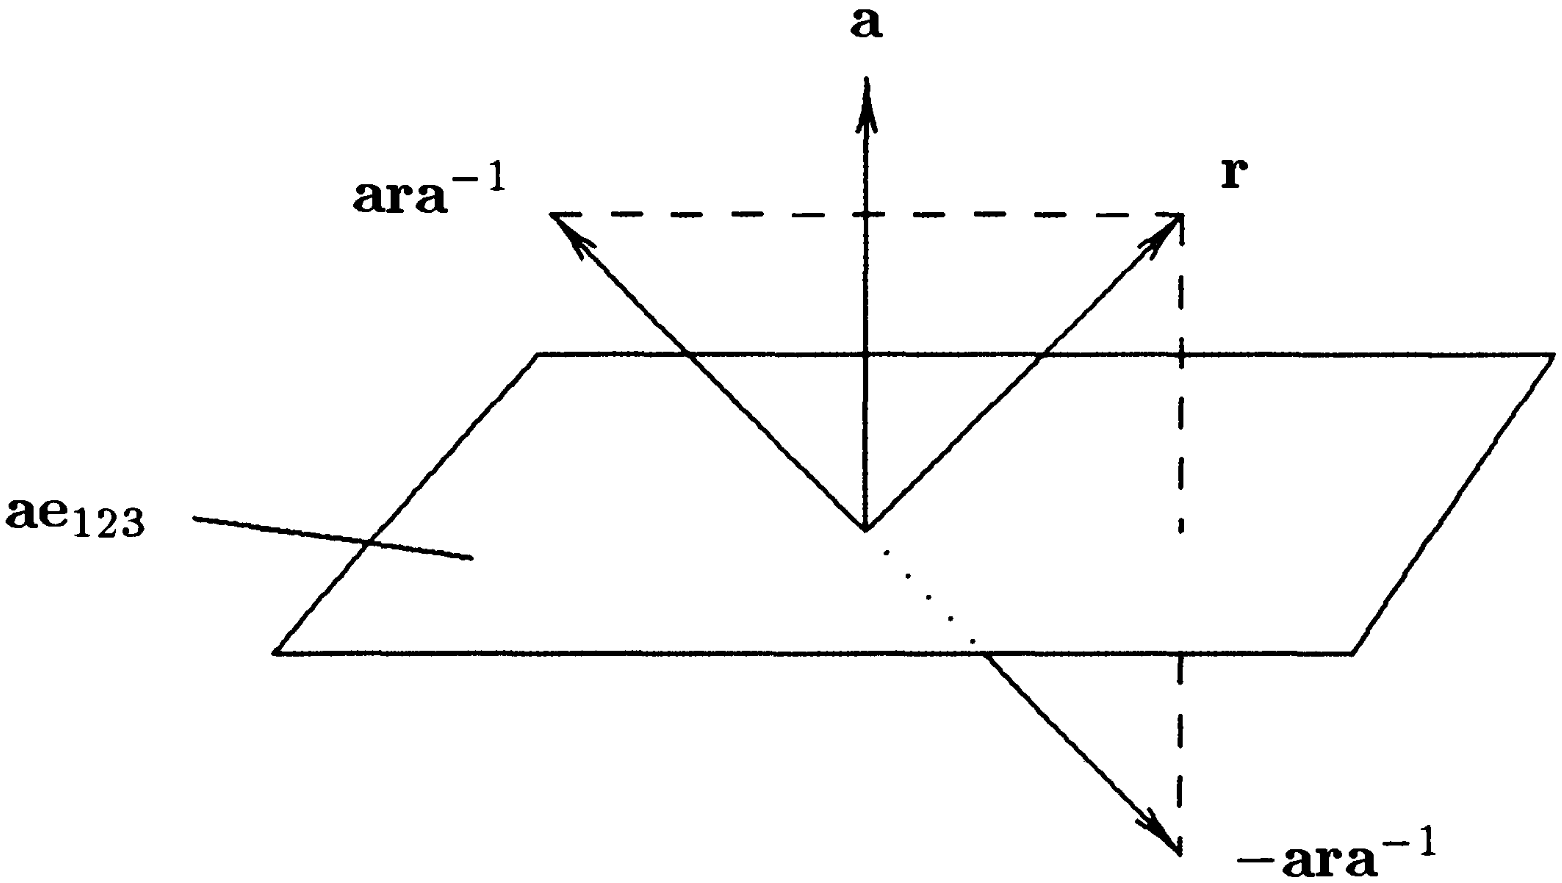
\includegraphics[width=0.6\linewidth]{figures/rotacaoCl3.png}
		\end{center}
		\caption{Representação da reflexão de $\mathbf r$ por $\mathbf a$ \cite{lounestoClifford}.}
		\label{fig:rotacaoCl3}
	\end{figure}
	 
	 Duas reflexões sucessivas nos planos perpendiculares a $\mathbf a$ e $\mathbf b$ resultam em uma rotação $\mathbf r \rightarrow \mathbf b(\mathbf a\mathbf r\mathbf a^{-1})\mathbf b^{-1}$ ao redor do eixo que é perpendicular a ambos $\mathbf a$ e $\mathbf b$ (veja Figura~\ref{fig:rotacaoCl32}).
	 
	 \begin{figure}[H]
	 	\begin{center}
	 		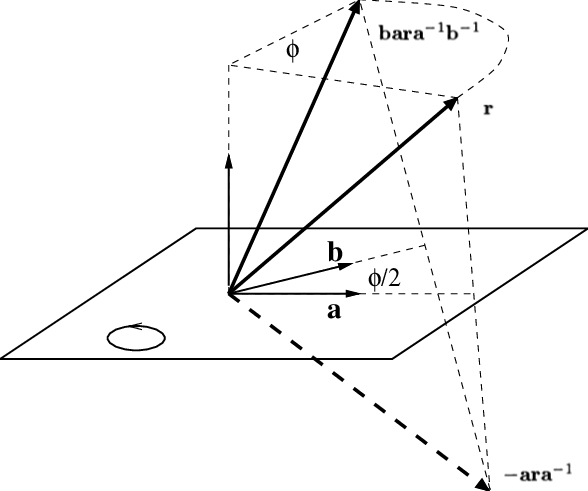
\includegraphics[width=0.6\linewidth]{figures/rotacaocl32.png}
	 	\end{center}
	 	\caption{Representação da rotação por duas reflexões}
	 	\label{fig:rotacaoCl32}
	 \end{figure}
	 
	\subsubsection{Partes pares e impares} 
	Assim como a álgebra exterior, a $\mathcal C \ell_3$ é uma soma direta de dois subespaços que chamamos de
	\begin{enumerate}
		\item parte par $\mathcal C \ell_3^+$: $\bigwedge^0\mathbb{R}^3 \oplus \bigwedge^2\mathbb{R}^3$ e
		\item a parte ímpar $\mathcal C \ell_3^-$: $\bigwedge^1\mathbb{R}^3\oplus \bigwedge^3\mathbb{R}^3$.
	\end{enumerate}
	Para ambas as álgebras, a parte par também é uma subálgebra. A subálgebra par $(\bigwedge\mathbb{R}^3)^+ = \mathbb{R} \oplus \bigwedge^2\mathbb{R}^3$ de $\bigwedge\mathbb{R}^3$ é comutativa, porém, a subálgebra $\mathcal C \ell_3^+ = \mathbb{R} \oplus \bigwedge^2\mathbb{R}^3$ de $\mathcal C \ell_3$ não é.
	
	Na verdade, a subálgebra $\mathcal C \ell_3^+$ nos interessa bastante. Os elementos gerados por $1 \in \mathbb{R}$ e pelos bivetores $\mathbf e_1\mathbf e_2$, $\mathbf e_3\mathbf e_1$ e $\mathbf e_2\mathbf e_3 \in \bigwedge^2\mathbb{R}^3$ são chamados pares, porque são produtos de um número par de vetores (lembrando que 0 é par). Esses elementos pares são escritos como $$w+x\mathbf e_2\mathbf e_3 + y \mathbf e_3\mathbf e_1+z\mathbf e_1\mathbf e_2$$ e formam um subespaço real $$\mathbb{R}\oplus\bigwedge^2\mathbb{R}^3 = \{w+x\mathbf e_2\mathbf e_3 + y \mathbf e_3\mathbf e_1+z\mathbf e_1\mathbf e_2 \ | \ w,x,y,z \in \mathbb{R} \}$$
	que é fechado sobre a multiplicação e, portanto, o subespaço $\mathbb{R}\oplus \bigwedge^2\mathbb{R}^3$ é de fato uma subálgebra. Na verdade, essa subálgebra é isomorfa ao anel de divisão dos quatérnios $\mathbb{H}$ (que abordaremos melhor na próxima seção) através da correspondência
	$$ \mathbf e_2\mathbf e_3 \rightarrow i,\quad \mathbf e_1\mathbf e_2 \rightarrow j, \quad \mathbf e_3\mathbf e_1 \rightarrow k.$$
	
	\newpage
	
	\subsection{Álgebra dos Quatérnios}
	William Rowan Hamilton foi uma criança extremamente precoce. De origem irlandesa, viveu entre 1805 e 1865 e aos três anos de idade já lia perfeitamente em inglês \cite{BoyerMathHistory}. Devido a morte antecipada de seus pais, teve como orientador um tio linguista e aos seus cinco anos já sabia latim e hebraico. Até os dez anos já era familiarizado com italiano, francês, árabe, sânscrito, persa, caldeu e algumas outras línguas orientais. Ainda criança, Hamilton demonstrou grande interesse pela matemática, influenciado por autores como Newton e Laplace caminhava a passos largos para o mundo da física e astronomia. Trata-se de um dos grandes nomes da ciência do século XIX \cite{AlgebraAbstrata2BienalSBM}.
	
	Hamilton percebeu que uma notação utilizada na teoria dos números complexos não era a mais adequada, pois a expressão $a + bi$ não era realmente uma soma, isto é, não é como somar dois números reais que pertencem a mesma dimensão --- o que dá sentido a soma. Dessa forma, Hamilton estava convencido de que o sinal ‘$+$’ é um equívoco, um acidente histórico, e que as duas partes não podiam ser naturalmente somadas. A partir deste pensamento, publicou em 1833 a teoria de números complexos formalmente como conhecemos hoje, definindo a soma e produto em pares ordenados da forma
	\begin{equation*}
		(a,b) + (c,d) = (a + b, c + d)
	\end{equation*}
	\begin{equation*}
		(a, b)(c, d) = (ac-bd, ad + bc)
	\end{equation*}
	
	Visto sua proximidade com a física, Hamilton percebeu como esta nova abordagem permitiria uma visão dos números complexos como entidades orientadas no plano e se perguntou como seria esta relação se fosse expandida para o espaço tridimensional. Infelizmente as respostas não foram fáceis e por dez anos trabalhou tentando desenvolver ternas  que pudessem ser multiplicadas com as propriedades que desejava. Na verdade, Hamilton jamais poderia encontrar sua terna, como é apresentado em \cite{lounestoClifford}. 
	
	Em 1843, Hamilton andava ao lado de sua esposa na ponte Brougham sobre o Royal Canal a caminho de presidir uma reunião do Conselho da Real Sociedade da Irlanda e dividia-se entre conversas ocasionais e no pensar sobre seu trabalho. Lá teve um \textit{insight}: percebeu que poderia ter sua generalização se utilizasse quádruplas em vez de ternas e ignorasse a comutatividade para a multiplicação. Percebeu que para quádruplas $a + bi + cj + dk$ teria as leis
	\begin{equation}\label{eq:quat}
		i^2 = j^2 = k^2 = ijk = -1.
	\end{equation}
	
	\begin{definicao}[Quatérnio]
		Seja $\{i,j,k\}$ a base do $\mathbb{R}^3$. Um \textit{quatérnio} é definido como um elemento da forma $$q=q_0+\mathbf{q_v},$$
		onde $q_0 \in \mathbb{R}$ é um escalar e $\mathbf{qv}=q_1\mathbf{i}+q_2\mathbf{j}+q_3\mathbf{k}$ é um vetor de $\mathbb{R}^3$.
	\end{definicao}
	
	Ou seja, todo elemento $q$ da forma $q = q_0 + q_1\textbf{i} + q_2\textbf{j} + q_3\textbf{k}$ é um quatérnio e a medida que variamos os valores dos coeficientes reais $q_0, q_1, q_2$ e $q_3$ independentemente uns dos outros geramos o \textit{conjunto numérico dos Quatérnios} $\mathbb{H}$. 
	
	\begin{definicao}[Adição]
		Dados dois quatérnios $p=p_0+\mathbf{p_v}$ e $q=q_0+\mathbf{q_v}$ em $\mathbb{H}$, define-se a adição de $p$ a $q$ como  
		$$p+q=(p_0+q_0)+(\mathbf{p_v}+\mathbf{q_v})$$
	\end{definicao}
	
	\begin{proposicao}
		O conjunto $\mathbb{H}$ é fechado para adição.
		\begin{proof}
			Considerando $r=p+q$, podemos escrever o elemento $r$ como
			$$r=r_0+\mathbf{r_v}$$
			onde sua parte escalar é dada por $r_0=p_0+q_0$ e sua parte vetorial é dada por $\mathbf{r_v=p_v+q_v}$.
		\end{proof}
	\end{proposicao}

	\begin{proposicao}
		($\mathbb{H},+$) é um grupo abeliano.
		\begin{proof}
			Dados $p,q,r \in \mathbb{H}$, temos que
			$$(p+q)+r=[(p_0+\mathbf{p_v})+(q_0+\mathbf{p_v})]+(r_0+\mathbf{r_v})=$$$$[(p_0+q_0)+(\mathbf{p_v}+\mathbf{q_v})]+(r_0+\mathbf{r_v})=$$$$[(p_0+q_0+r_0)+(\mathbf{p_v}+\mathbf{q_v}+\mathbf{r_v})]=$$$$\{[p_0+(q_0+r_0)]+[\mathbf{p_v}+(\mathbf{q_v}+\mathbf{r_v})]\}=$$$$(p_0+\mathbf{p_v})+[(q_0+r_0)+(\mathbf{q_v}+\mathbf{r_v})]=$$$$(p_0+\mathbf{p_v})+[(q_0+\mathbf{q_v})+(r_0+\mathbf{r_v})]=p+(q+r),$$ donde é associativa.
			
			\noindent Também temos que $$p+q=(p_0+\mathbf{p_v})+(q_0+\mathbf{q_v})=(p_0+q_0)+(\mathbf{p_v}+\mathbf{q_v})=(q_0+p_0)+(\mathbf{q_v}+\mathbf{p_v})=q+p,$$ isso é, é comutativa.
			
			\noindent Seja $0_{\mathbb{H}}=0+\mathbf{0_v}$. Como $$p+0_{\mathbb{H}}=(p_0+\mathbf{p_v})+(0+\mathbf{0_v})=(p_0+0)+(\mathbf{p_v}+\mathbf{0_v})=$$$$(0+p_0)+(\mathbf{0_v}+\mathbf{p_v})=p_0+\mathbf{p_v},$$ então existe um elemento neutro, a saber, $0_{\mathbb{H}}$.
			
			\noindent Também existe elemento oposto, afinal, $$p+(-p)= (p_0+\mathbf{p_v})+(-p_0-\mathbf{p_v})=[p_0+(-p_0)]+[\mathbf{p_v}+(\mathbf{-p_v})]=$$$$(p_0-p_0)+(\mathbf{p_v}-\mathbf{p_v})=0+\mathbf{0_v}=0_{\mathbb{H}}.$$
		\end{proof}
	\end{proposicao}
	
	\begin{definicao}[Multiplicação por escalar]
		Dado um quatérnio $q=q_0+\mathbf{q_v} \in \mathbb{H}$ e uma constante escalar real $\alpha \in \mathbb{R}$, define-se a multiplicação de $q$ pelo escalar $\alpha$ da forma
		$$\alpha q=(\alpha q_0)+(\alpha \mathbf{q_v})$$
	\end{definicao}
	
	\begin{proposicao}
		O conjunto $\mathbb{H}$ é fechado para a multiplicação de escalares reais.
		\begin{proof}
			Podemos considerar tal multiplicação como o elemento 
			\begin{equation*}
				r=r_0+\mathbf{r_v}
			\end{equation*}
			onde sua parte escalar é dada por $r_0=\alpha q_0 \in \mathbb{R}$ e sua parte vetorial é dada por $\mathbf{r_v}=\alpha \mathbf{q_v} \in \mathbb{R}^3$.
		\end{proof}
	\end{proposicao}
	
	\begin{proposicao}
		$\mathbb{H}$ é um espaço vetorial sobre o corpo $\mathbb{R}$.
		\begin{proof}
			Dados os números reais $\alpha,\beta$ e os quatérnios $p$ e $q$, temos que $$(\alpha \beta)q=(\alpha \beta)(q_0+\mathbf{q_v})=\alpha \beta q_0+\alpha \beta \mathbf{q_v}=\alpha(\beta q_0+\beta \mathbf{q_v})=\alpha(\beta q),$$ então é associativa.
			
			\noindent Também, como $$1q=1(q_0+\mathbf{q_v})=(1q_0+1\mathbf{q_v})=q_0+\mathbf{q_v}=q,$$ então $1q=q$.
			
			\noindent A operação também é distributiva em relação à soma, pois $$((\alpha + \beta)q_0 + (\alpha + \beta)\mathbf{q_v})=\alpha(q_0+\mathbf{q_v})+\beta(q_0+\mathbf{q_v})=\alpha q+\beta q.$$ O análogo para $\alpha q+\beta q$ vale. Além disso, aplicando as devidas distributividades, temos que $\alpha p+\alpha q=(\alpha p_0+\alpha\mathbf{p_v})+(\alpha q_0+\alpha\mathbf{q_v})=\alpha p+\alpha q$. Mostra-se de forma análoga que $\alpha p+\alpha q$.
		\end{proof}
	\end{proposicao}
	
	\begin{proposicao}
		$\mathbb{H} \simeq \mathbb{R}^4$.
	\end{proposicao}

	Na verdade, historicamente esse isomorfismo vem de que o calculo vetorial como conhecemos hoje, onde define-se $\mathbb{R}^4$, é mera simplificação das ideias de Hamilton sobre quatérnios. Simplificação feita por Josiah Willard Gibbs (1839 – 1903) em um conjunto de notas para seus estudantes de física-matemática intitulado Elements of Vector Analysis \cite{AlgebraAbstrata2BienalSBM}.
	\\
	
	\begin{definicao}[Quatérnio conjugado]
		Seja $q = q_0 + \mathbf{q_v} \in \mathbb{H}$, define-se seu \textit{conjugado} como $q^* = q_0 - \mathbf{q_v}$.
	\end{definicao}
	
	\subsubsection{Produto algébrico de quatérnios}
	Tendo as estruturas algébricas já estabelecidas, pode-se construir uma terceira operação dos quatérnios, baseando-se em \cite{QuaterniosAndRotationsKuipers}. Trata-se do \textit{produto algébrico dos quatérnios}, que causou os dez anos de trabalho para Hamilton e que torna sua álgebra um tanto não trivial por conta da falta de comutatividade.
	\\
	
	Suponha dois elementos $p = p_0 + \mathbf{p_v}$ e $q = q_0 + \mathbf{q_v}\in \mathbb{H}\setminus0$. Sabe-se que podemos escrever $\mathbf{p_v} = p_1\mathbf{i} + p_2\mathbf{j} + p_3\mathbf{k}$ e $\mathbf{q_v} = q_1\mathbf{i} + q_2\mathbf{j} + q_3\mathbf{k}$. Se multiplicarmos os dois elementos termo a termo, como na propriedade distributiva, teremos:
	\begin{equation}
		\begin{aligned}
			pq = (p_0+\mathbf{i}p_1+\mathbf{j}p_2+\mathbf{k}p_3)(q_0+\mathbf{i}q_1+\mathbf{j}q_2+\mathbf{k}q_3) \\ = (p_0q_0+p_0+\mathbf{i}p_0q_1+p_1q_0)+\mathbf{j}(p_0q_2+p_2q_0) \\ +\mathbf{k}(p_0q_3+p_3q_0)+\mathbf{i}^2p_1q_1+\mathbf{j}^2p_2q_2+\mathbf{k}^2p_3q_3+\mathbf{ij}p_1q_2+\mathbf{ji}p_2q_1 \\ +\mathbf{ik}p_1q_3+\mathbf{ki}p_3q_1+\mathbf{jk}p_2q_3+\mathbf{kj}p_3q_2
		\end{aligned}		   	       
	\end{equation}
	Mas podemos utilizar das regras definidas na equação~\ref{eq:quat} para simplificar essa expressão. Historicamente, os produtos dos versores a seguir foram definidos por Hamilton por construção a partir de seus três planos retangulares intersectados utilizando de rotações \cite{QuaterniosHamilton}, mas aproveitaremos a correspondência de $i,j,k$ com os elementos de $\mathcal C \ell_3$. Temos que
	\begin{equation*}
		\mathbf{ij} \rightarrow \mathbf e_2\mathbf e_3\mathbf e_1\mathbf e_2 = \mathbf e_3\mathbf e_1 \rightarrow \mathbf{k} = \mathbf{-ji}
	\end{equation*}
	\begin{equation*}
		\mathbf{jk} \rightarrow \mathbf e_1\mathbf e_2\mathbf e_3\mathbf e_1 = \mathbf e_2\mathbf e_3 \rightarrow \mathbf{i} = \mathbf{-kj}
	\end{equation*}
	\begin{equation*}
		\mathbf{ki} \rightarrow \mathbf e_3\mathbf e_1\mathbf e_2\mathbf e_3 = \mathbf e_1\mathbf e_2 \rightarrow \mathbf{j} = \mathbf{-ik}
	\end{equation*}
	Assim, nosso produto fica
	\begin{equation}
		\begin{aligned}
			pq = (p_0q_0-p_1q_1+p_2q_2+p_3q_3)+p_0(\mathbf{i}q_1+\mathbf{j}q_2+\mathbf{k}q_3+q_0(\mathbf{i}p_1+\mathbf{j}p_2+\mathbf{k}p_3) \\ +\mathbf{i}(p_2q_3-p_3q_2)+\mathbf{j}(p_3q_1-p_1q_3)+\mathbf{k}(p_1q_2-p_2q_1).
		\end{aligned}
	\end{equation}
	Perceba que a parte real quase representa o produto interno $<\mathbf{p_v}, \mathbf{q_v}> = p_1q_1 + p_2q_2 + p_3q_3$, então, pode-se reescrever a expressão como
	\begin{equation}
		\begin{aligned}
			pq = p_0q_0-<\mathbf{p_v,q_v}>+p_0\mathbf{q_v}+q_0\mathbf{p_v}+\mathbf{i}(p_2p_3-p_3p_2)+\mathbf{j}(p_3q_1-p_1q_3)\\+\mathbf{k}(p_1q_2-p_2q_1)
		\end{aligned}
	\end{equation}
	
	E, por fim, perceba que o produto vetorial $\mathbf{p_v} \times \mathbf{q_v} = \mathbf{i}(p_2q_3 - p_3q_2) + \mathbf{j}(p_3q_1 - p_1q_3) + \mathbf{k}(p_1q_2 - p_2q_1)$ aparece no nosso produto, donde podemos reescrevê-lo como
	\begin{equation*}
		pq=p_0q_0\,-<\mathbf{p_v,q_v}>+p_0\mathbf{q_v}+q_0\mathbf{p_v}+\mathbf{p_v}\times\mathbf{q_v}.
	\end{equation*}
	
	\begin{proposicao}
	    O conjunto dos quatérnios é fechado pelo produto algébrico de quatérnios.
		\begin{proof}
			Como o quatérnio produto algébrico $r=pq$ pode ser escrito como 
			\begin{equation}
				r=r_0+\mathbf{r_v},
			\end{equation}
			onde $r_0=(p_0q_0-<\mathbf{p_v,q_v}>)$ e $\mathbf{r_v}=(p_0\mathbf{q_v}+q_0\mathbf{p_v}+\mathbf{p_v}\times\mathbf{q_v})$, então $r \in \mathbb{H}$.
		\end{proof}
	\end{proposicao}
	
	\begin{proposicao}
		O produto algébrico de quatérnios é associativo. Ou seja, dados $p,q,r \in \mathbb{H}$, temos que 
		\begin{equation*}
			(pq)r=p(qr)
		\end{equation*}
	\end{proposicao}
	
	\begin{proposicao}
		O produto algébrico de quatérnios é distributivo em relação à adição, ou seja, para $p,q,r \in \mathbb{H}$
		\begin{equation*}
			p(q+r)=pq+pr \,\,\,\,\,\,\,\,e\,\,\,\,\,\,\,\, (p+q)r=pr+qr
		\end{equation*}	
	\end{proposicao}
	
	Assim, o conjunto dos quatérnios monido das operações de adição, multiplicação por escalar e do produto de quatérnios forma uma álgebra associativa, denominada \textit{Álgebra dos Quatérnios}.

	\begin{definicao}[Elemento neutro do produto]
		Seja $1_\mathbb{H} = 1 + \mathbf{0_v} \in \mathbb{H}$ o elemento da álgebra dos quatérnios definido como identidade do produto de quatérnios. Isto é, para todo $q = q_0 + \mathbf{q_v} \in \mathbb{H}$, $q1_\mathbb{H} = q$.
	\end{definicao}
	
	\begin{proposicao}
		Sejam $p,q\in \mathbb{H}$. Então $(pq)^* = q^*p^*$.
	\end{proposicao}
	
	\begin{definicao}[Norma]
		Dado $q \in \mathbb{H}$, sua \textit{norma} é dada por $N(q) = q^*q$. 	
	\end{definicao}
	
	\begin{proposicao}
		Dado $p \in \mathbb{H}$, a norma do conjugado de $p$ é igual a sua própria norma, ou seja, $N(p^*) = N(p)$.
	\end{proposicao}
	
	\begin{proposicao}
		Sejam $p, q \in \mathbb{H}$, a norma do produto $pq$ é igual ao produto das normas de $p$ e $q$, isto é, $N(pq) = N(p)N(q)$.
	\end{proposicao}
	
	\begin{definicao}[Inverso]
		Para cada $q\in \mathbb{H}\setminus\{0\}$, existe um elemento $q^{-1}\in \mathbb{H}$ tal que $qq^{-1} = q^{-1}q = 1_\mathbb{H}$ e que $q^{-1} = \dfrac{1}{N^2(q)}q^*$ chamado de \emph{inverso do quatérnio $q$}.
	\end{definicao}
	
	\begin{proposicao}
		Seja $q$ um quatérnio. Se $q$ é unitário, isso é, $N(q) = 1$, então seu inverso coincide com seu conjugado: $$q^{-1} = q^*.$$
	\end{proposicao}
	
	\begin{definicao}[Quatérnio puro]
		O quatérnio $q$ é dito \emph{quatérnio puro} quando sua parte real for zero. O conjunto dos quatérnios puros é denotado por $\mathbb{H}_0$.
	\end{definicao}

	\begin{proposicao}
		$\mathbb{H}_0 \simeq \bigwedge^2\mathbb{R}^3 \simeq \mathbb{R}^3$
	\end{proposicao}

	\begin{definicao}[Quatérnio real]
		O quatérnio $q$ é dito \emph{quatérnio real} quando sua parte vetorial for o elemento nulo. O conjunto dos quatérnios reais é denotado por $\mathbb{R}$, visto que é trivialmente isomorfo aos reais.
	\end{definicao}	
	
	\subsubsection{Rotação com quatérnios}
	
	\begin{teorema}\label{teo:rotacaoQuaternios}
		Seja $p_{\mathbf x}\in \mathbb{H}_0$ um quatérnio associado a um dado vetor $\mathbf x\in\mathbb{R}^3$. Então, o quatérnio unitário $q = \cos(\frac{1}{2}\theta) + \sin(\frac 1 2 \theta)\mathbf v$ induz uma rotação $\theta$ de $\mathbf x$ sobre o eixo $\langle \mathbf v\rangle$, determinando $\mathbf x'\in \mathbb{R}^3$, pelo mapa
		$$
		\begin{tabular}{rccl}
			$R_q$:&$\mathbb{H}_0$ & $\longrightarrow$ & $\mathbb{H}_0$\\
			&$p_{\mathbf x}$ & $\longmapsto$ & $p_{\mathbf x'} = R_q(\mathbf x) = qp_{\mathbf x}q^{-1}$
		\end{tabular}.
		$$
	\end{teorema}

	\begin{corolario}
		Sejam $q=q_0+\mathbf q_v\in \mathbb{H}$ e $\mathbf x\in \mathbb{R}^3$. O resultado da rotação $\mathbf x'$ de $\mathbf x$ por $R_q$ pode ser escrito como combinação linear da base $\{\mathbf x, \mathbf q_v,\mathbf q_v\times \mathbf x\}$ da forma $$\mathbf x' = (q_0^2 - \mathbf q_v\cdot \mathbf q_v)\mathbf x + 2(\mathbf q_v\cdot \mathbf x)\mathbf q_v+2q_0(\mathbf q_v\times \mathbf x).$$
		\begin{proof}
			Esse resultado é construído de forma detalhada em \cite{fidalgotese}.
		\end{proof}
	\end{corolario}
	
	\newpage
	
	 \documentclass[a4paper,12pt]{article}
\usepackage[a4paper,top=3cm,bottom=2cm,left=3cm,right=3cm,marginparwidth=1.75cm]{geometry}
\usepackage[brazil]{babel}
\usepackage[T1]{fontenc}
\usepackage[utf8]{inputenc}
\usepackage{amsmath}
\usepackage{amsthm}
\usepackage{MnSymbol}
\usepackage{wasysym}
\usepackage{hyperref}
\usepackage{color}
\definecolor{Blue}{rgb}{0,0,0.9}
\definecolor{Red}{rgb}{0.9,0,0}
\usepackage{esvect}
\usepackage{graphicx}
\usepackage{float}
\usepackage{indentfirst}
\usepackage{caption}
\usepackage{blkarray}
\newcommand\Mark[1]{\textsuperscript#1}
\usepackage{pgfplots}
\usepackage{amsfonts}
\usepackage[english, ruled, linesnumbered]{algorithm2e}
\usepackage{algorithmic}
\usepackage{enumitem}

\newcommand{\nucleoe}{\emph{\text{nu }}}
\newcommand{\nucleo}{\text{nu }}
\newcommand{\imageme}{\emph{\text{nu }}}
\newcommand{\imagem}{\text{nu }}

\theoremstyle{plain}
\newtheorem{teorema}{Teorema}[section]
\newtheorem{lema}{Lema}[section]
\newtheorem{proposicao}{Proposição}[section]
\newtheorem{corolario}{Corolário}[section]

\theoremstyle{definition}
\newtheorem{definicao}{Definição}[section]
\newtheorem{observacao}{Observação}[section]
\newtheorem{exemplo}{Exemplo}[section]

\newenvironment{solucao}
{\renewcommand\qedsymbol{$\triangle$}\begin{proof}[Solução]}{\end{proof}}

\title{\textsc{Relações e Operações Binárias}\\ \textsl{um resumo}}
\author{Guilherme Philippi}
\begin{document}
\maketitle
	
Apresenta-se nesse texto um compilado de definições e resultados envolvendo os conceitos de relações entre conjuntos e operações binárias. Tudo que aqui se apresenta fora extraído de \cite{johnAlgebra, michalAlgebra, maierAlgebra}, principalmente de \cite{johnAlgebra}.
	
\section{Produto Cartesiano e Relações}

\begin{definicao}[Produto cartesiano]
	Sejam $A$ e $B$ conjuntos. O conjunto $$A\times B = \{(a,b) \ | \ a\in A \text{ e } b\in B\}$$
	é o \emph{produto cartesiano de A e B}.
\end{definicao}

\begin{exemplo}
	Se $A = \{1,2,3\}$ e $B = {3,4}$, então $$A\times B = \{(1,3),(1,4),(2,3),(2,4),(3,3),(3,4)\}.$$
\end{exemplo}

\begin{definicao}[Relação]
	Uma	\emph{relação} entre dois conjuntos $A$ e $B$ é um subconjunto $\mathcal{R}\subset A\times B$. Lê-se $(a,b) \in \mathcal{R}$ como ``$a$ está relacionado com $b$'' e escreve-se $a\mathcal{R}b$.
\end{definicao}

\begin{exemplo}[Relação de igualdade]\label{ex:igualdade}
	A realação $=$, chamada \emph{relação de igualdade}, é definida sobre um conjunto $S$ por $$= \text{é o subconjunto } \{(x,x) \ |\ x\in S\}\subset S\times S.$$
\end{exemplo}

\begin{observacao}
	Sempre que uma relação for definida entre um conjunto $S$ e ele mesmo, como no exemplo~\ref{ex:igualdade}, diremos que esta é uma relação \emph{sobre} $S$.
\end{observacao}

\begin{definicao}[Função]
		Uma \emph{função} $\varphi$ que mapeia $X$ em $Y$ é uma relação entre $X$ e $Y$ com a propriedade de que cada $x\in X$ só irá aparecer uma única vez, e exatamente uma, em um par ordenado $(x,y)\in \varphi$. Também chamamos $\varphi$ de \emph{mapa} ou \emph{mapeamento} de $X$ em $Y$. Escrevemos $\varphi: X\longrightarrow Y$ e expressaremos $(x,y)\in\varphi$ por $\varphi(x) = y$. O \emph{domínio} de $\varphi$ é o conjunto $X$ e o conjunto $Y$ é dito \emph{contradomínio} de $\varphi$. Chama-se de \emph{alcance} de $\varphi$ o conjunto $\varphi[X] = \{\varphi(x)\ | \ x \in X\}.$
\end{definicao}

\begin{definicao}[Função injetiva e sobrejetiva]
		Uma função $\varphi: X \longrightarrow Y$ é \emph{injetiva} se $\varphi(x_1) = \varphi(x_2) \iff x_1 = x_2$. Também, $\varphi$ é dita \emph{sobrejetiva} se o alcance de $\varphi$ é $Y$. Se uma função é injetiva e sobrejetiva, então dizemos que a função é \emph{bijetiva}.
\end{definicao}

\begin{definicao}
	Sejam $S$ um conjunto $\mathcal{R}$ uma relação sobre $S$.
	Dizemos que $\mathcal{R}$ é uma relação
	\begin{enumerate}
		\item \emph{(reflexiva).} se $a\mathcal{R}a$, para todo $a\in S$;
		\item \emph{(simétrica).} se para todo $a,b \in S$ $a\mathcal{R}b \iff b\mathcal{R}a$;
		\item \emph{(antissimétrica).} se $a\mathcal{R}b$ e $b\mathcal{R}a \implies a = b$, para todo $a,b \in S$;
		\item \emph{(transitiva).} se $a\mathcal{R}b$ e $b\mathcal{R}c \implies a\mathcal{R}c$, $\forall \ a,b,c\in S$.
	\end{enumerate}
\end{definicao}


\section{Relações de Equivalência e Partições}

\begin{definicao}[Partições]
	Seja \(S\) um conjunto. Uma \emph{particão} \(P\) de
	\(S\) é uma subdivisão de \(S\) em subconjuntos não vazios e não
	sobrepostos, isto é, uma união de conjuntos disjuntos.	
\end{definicao}

\begin{exemplo}
	Pode-se particionar o conjunto dos números inteiros
	\(\mathbb{Z}\) na união de disjuntos \(P\cup I\), onde
	\(P = \{z \in \mathbb{Z} \ |\ z \text{ é par}\}\) e
	\(I = \{z \in \mathbb{Z} \ |\ z \text{ é impar}\}\).
\end{exemplo}

\begin{definicao}[Relação de equivalência]
	Uma \emph{relação de equivalência} $\sim$ sobre um conjunto
	\(S\) é uma relação que precisa ser, para todo $a,b,c\in S$,
	\begin{enumerate}
		\item \emph{(Transitiva).} Se \(a\sim b\) e \(b\sim c\), então \(a\sim c\);
		\item \emph{(Simétrica).} Se \(a\sim b\), então \(b\sim a\);
		\item \emph{(Reflexiva).} \(a\sim a\).
	\end{enumerate}
\end{definicao}

\begin{observacao}
	A noção de partição em \(S\) e a relação de equivalência em \(S\) são
	lógicamente equivalentes: Dada uma partição \(P\) sobre \(S\), pode-se
	definir uma relação de equivalência \(R\) tal que, se \(a\) e \(b\)
	estão no mesmo subconjunto partição, então \(a\sim b\) e, dada uma
	relação de equivalência \(R\), podemos definir uma partição \(P\) tal
	que o subconjunto que contêm \(a\) é o conjunto de todos os elementos
	\(b\) onde \(a\sim b\). Esse subconjunto é chamado de \emph{classe de
		equivalência de \(a\)}
	\[C_a = \{b\in S \ | \ a\sim b\}\]
	e \(S\) é particionado em classes de equivalência.
\end{observacao}

\begin{proposicao}
	Sejam \(C_a\) e \(C_b\) duas classes de equivalência do conjunto \(S\). Se existe \(d\) tal que \(d\in C_a\) e \(d\in C_b\), então \(C_a = C_b\).
\end{proposicao}

\begin{observacao}[Representante]
	Seja um conjunto \(S\). Suponha que exista uma relação de equivalência
	ou uma partição sobre \(S\). Então, pode-se construir um novo conjunto
	\(\bar{S}\) formado pelas classes de equivalência ou os subconjuntos
	partições de \(S\). Essa construção induz uma notação muito útil: para
	\(a\in S\), a classe de equivalência de \(a\) ou o subconjunto partição
	que contém \(a\) serão denotados como o elemento
	\(\bar{a} \in \bar{S}\). Desta forma, a notação \(\bar{a} = \bar{b}\)
	significa que \(a \sim b\) e chamamos \(a,b \in S\) de
	\emph{representantes} das respectivas classes de equivalência
	\(\bar{a}, \bar{b} \in \bar{S}\).
\end{observacao}

\begin{definicao}
	Seja um mapeamento \(\varphi: S \longrightarrow T\).
	Chama-se de \emph{relação de equivalência determinada por \(\varphi\)} a
	relação dada por \(\varphi(a) = \varphi(b) \Rightarrow a \sim b\). Além
	disso, para um elemento \(t\in T\), o subconjunto de
	\(\varphi^{-1}(t) = \{s \in S\ | \ \varphi(s) = t\}\) é dito
	\emph{imagem inversa de \(t\) por \(\varphi\)}.
\end{definicao}

\begin{proposicao}
	Seja um mapeamento \(\varphi: S \longrightarrow T\)
	e \(t \in T\) um elemento qualquer de \(T\). Se a imagem inversa
	\(\varphi^{-1}(t)\) é não vazia, então \(t \in \text{im}\ \varphi\) e
	\(\varphi^{-1}(t)\) forma uma classe de equivalência
	\(\bar{\varphi}\in \bar{S}\) através da relação determinada por
	\(\varphi\).	
\end{proposicao}

\section{Operações binárias}

\begin{definicao}[Operação binária]
	Uma \emph{operação binária} sobre um conjunto \(S\) é uma função \(*: S\times S \longrightarrow S\).
\end{definicao}

\begin{observacao}[Notação de operação]
	Usaremos a notação \(*(a,b) = a*b\), para simplificar a escrita de
	propriedades. Também, quando não houver ambiguidade, suprimiremos o simbolo da operação, fazendo $a*b = ab$.
\end{observacao}


\begin{definicao}
	Para $a,b,c \; \in S$, uma operação binária $*$ é dita
	
	\begin{itemize}
		\item \emph{Associativa}, se $(a*b)*c = a*(b*c)$;
		\item \emph{Comutativa}, se \(a*b = b*a\).
	\end{itemize}
\end{definicao}

\begin{proposicao}
	Seja uma operação associativa dada sobre o conjunto
	\(S\). Há uma única forma de definir, para todo inteiro \(n\), um
	produto de \(n\) elementos \(a_1,\dots,a_n \in S\) (diremos
	\([a_1\dotsb a_n]\)) com as seguintes propriedades:
	
	\begin{enumerate}
		\def\labelenumi{\arabic{enumi}.}
		\item
		o produto \([a_1]\) de um elemento é o próprio elemento;
		\item
		o produto \([a_1a_2]\) de dois elementos é dado pela operação binária;
		\item
		para todo inteiro \(1\leq i\leq n\),
		\([a_1\dotsb a_n] = [a_1\dotsb a_i][a_{i+1}\dotsb a_n]\).
	\end{enumerate}
\end{proposicao}

\begin{proof}
	A demonstração dessa proposição é feita por indução em \(n\).
\end{proof}

\begin{definicao}
	Dizemos que \(e\in S\) é \emph{identidade} para uma operação binária se \(ea = ae = a\) para todo \(a\in S\).
\end{definicao}

\begin{proposicao}
	O elemento identidade é único.
\end{proposicao}
\begin{proof}
	Se \(e,e'\) são identidades, já que \(e\) é identidade, então \(ee' = e'\) e, como $e'$ é uma identidade, \(ee' = e\). Logo \(e = e'\), isto é, a identidade é única.
\end{proof}

\begin{observacao}
	Usaremos $\vec{1}$ para representar a identidade multiplicativa e $\vec{0}$ para denotar a aditiva.
\end{observacao}

\begin{definicao}[Elemento inverso]
	Seja uma operação binária que possua uma identidade. Um elemento \(a\in S\) é chamado \emph{invertível} se há um outro elemento \(b\in S\) tal que \(ab = ba = 1\). Desde que \(b\) exista, ela é única e a denotaremos por \(a^{-1}\) e a chamaremos
	\emph{inversa de $a$}.
\end{definicao}


\begin{proposicao}
	Se \(a,b\in S\) possuem inversa, então a composição \((ab)^{-1} = b^{-1}a^{-1}\).
\end{proposicao}

\begin{observacao}[Potências]
	Usaremos as seguintes notações:
	\begin{itemize}
		\item \(a^n = a^{n-1}a\) é a composição de \(a\dotsb a\) \(n\) vezes;
		\item \(a^{-n}\) é a inversa de \(a^n\);
		\item \(a^0 = \vec{1}\).
	\end{itemize}
	
	Com isso, tem-se que \(a^{r+s} = a^ra^s\) e \((a^r)^s = a^{rs}\). (Isso
	não induz uma notação de fração \(\frac{b}{a}\) a menos que seja uma operação
	comutativa, visto que \(ba^{-1}\) pode ser diferente de \(a^{-1}b\)).
	Para falar de uma operação aditiva, usaremos \(-a\) no lugar de
	\(a^{-1}\) e \(na\) no lugar de \(a^n\).
\end{observacao}

\phantomsection
\addcontentsline{toc}{chapter}{Referências Bibliográficas}

\bibliographystyle{unsrt}
\bibliography{references}

\end{document}
	
	\newpage
	\chapter{Materiais e Métodos\label{sec:materiais}}
	
	No capítulo anterior introduzimos a Álgebra dos Quatérnios e a abordagem clássica do algorítimo Branch-and-Prune que soluciona o problema de geometria de distâncias moleculares discretizável utilizando matrizes. Neste capítulo, central para este trabalho, redefine-se este algorítimo trocando seu núcleo matricial por elementos da álgebra de quatérnios.
	
	\section{BP com Quatérnios}\label{sec:bpQ}
	
	Seja $G = (V,E,d)$ o grafo ponderado associado ao DMDGP. Usaremos as mesmas definições de distâncias, ângulos planos e ângulos de torção apresentados na seção~\ref{sec:bp}. Esta seção foi fortemente baseada nos trabalhos de Fidalgo \cite{agacse?} e Thompson \cite{thompsonBi}.
	
	\subsubsection*{Inicialização}
	
	Vamos remontar as matrizes $B_1$, $B_2$ e $B_3$ apresentadas na seção~\ref{sec:bp} em termos de quatérnios. Lembrando, como a matriz 
	$$B_1\: =\:
	\begin{bmatrix}
		1 & 0 & 0 & 0\\ 
		0 & 1 & 0 & 0\\ 
		0 & 0 & 1 & 0\\ 
		0 & 0 & 0 & 1
	\end{bmatrix},$$
	então ela é a identidade. Isso é, para representá-la nos quatérnios como $q_1 \in \mathbb{H}$, basta tomarmos o elemento neutro do produto $1_\mathbb{H} = 1 + \mathbf 0 \in \mathbb{H}$. Assim, nossa realização $\mathbf x_1$ do primeiro vértice, antes calculado como $$
	\begin{bmatrix}
		x_{1,1}\\ 
		x_{1,2}\\ 
		x_{1,3}\\ 
		1
	\end{bmatrix}
	= B_{1}\begin{bmatrix}
		0\\ 
		0\\ 
		0\\ 
		1
	\end{bmatrix} = 
	\begin{bmatrix}
	0\\ 
	0\\ 
	0\\ 
	1
	\end{bmatrix} \implies \mathbf x_1 = (0,0,0),
	$$
	
	agora é dado pelo conjugado $$\mathbf x_1 = q_1\mathbf 0q_1^* = 1_\mathbb{H}(0,0,0,0)1_\mathbb{H} = (0,0,0,0) \implies \mathbf x_1 = (0,0,0).$$
	
	Relembrando a matriz	
	$$B_2\: =\:
	\begin{bmatrix}
		-1 & 0 & 0 & -d_{1,2}\\
		0 & 1 & 0 & 0\\ 
		0 & 0 & -1 & 0\\ 
		0 & 0 & 0 & 1
	\end{bmatrix},$$
	podemos tentar enxergar quais operações ela compõe. Perceba que se multiplicarmos a matriz de rotação 
	$$R_{\mathbf j}(-\pi) =
	\begin{bmatrix}
		\cos(-\pi)&0 & -\sin(-\pi)& 0\\
		0 & 1 & 0& 0\\
		\sin(-\pi) & 0&\cos(-\pi)& 0\\
		0 & 0& 0& 1
	\end{bmatrix} = 
	\begin{bmatrix}
		-1&0 & 0& 0\\
		0 & 1 & 0& 0\\
		0 & 0&-1& 0\\
		0 & 0& 0& 1
	\end{bmatrix},
	$$
	que descreve a rotação de $-\pi$ ao redor do eixo $\mathbf j$, pela matriz de translação
	$$	
	T_{\mathbf i}(d_{1,2}) =
	\begin{bmatrix}
		1&0 & 0& d_{1,2}\\
		0 & 1 & 0& 0\\
		0 & 0&1& 0\\
		0 & 0& 0& 1
	\end{bmatrix}
	$$
	do espaço homogêneo que descreve a translação de $d_{1,2}$ sobre o eixo $\mathbf i$, teremos a matriz
	$$
	R_{\mathbf j}(-\pi)T_{\mathbf i}(d_{1,2}) = 
	\begin{bmatrix}
		-1&0 & 0& 0\\
		0 & 1 & 0& 0\\
		0 & 0&-1& 0\\
		0 & 0& 0& 1
	\end{bmatrix}
	\begin{bmatrix}
		1&0 & 0& d_{1,2}\\
		0 & 1 & 0& 0\\
		0 & 0&1& 0\\
		0 & 0& 0& 1
	\end{bmatrix}
	=
	\begin{bmatrix}
		-1 & 0 & 0 & -d_{1,2}\\
		0 & 1 & 0 & 0\\ 
		0 & 0 & -1 & 0\\ 
		0 & 0 & 0 & 1
	\end{bmatrix} = B_2.
	$$
	Isso é, as operações que compõem a $B_2$ tratam-se de uma rotação de $-\pi$ ao redor de $\mathbf j$ e uma translação de $d_{1,2}$ sobre $\mathbf i$. Portanto, para representarmos essas operações em um quatérnio, basta compormos as mesmas operações em $\mathbb{H}$.
	\\
	
	Segue do teorema~\ref{teo:rotacaoQuaternios} que o quatérnio unitário $$q_{\mathbf j} = \cos(\frac{-\pi}{2}) + \sin(\frac{-\pi} 2 )\mathbf j =  -\mathbf j$$ induz uma rotação ${-\pi}$ de $\mathbf x$ sobre o eixo $\langle \mathbf j\rangle$ ao tomarmos $q_{\mathbf j}\mathbf xq_{\mathbf j}^{-1}$. Mas como, para um quatérnio de rotação genérico 
	\begin{equation}
		q_{\mathbf v}^{-1} = 
		\cos \left(- \textstyle\frac{1}{2} \theta \right) + 
		\sin \left(- \textstyle\frac{1}{2} \theta \right)\mathbf v =
		\cos \left( \textstyle\frac{1}{2} \theta \right) - 
		\sin \left( \textstyle\frac{1}{2} \theta \right)\mathbf v = 
		q_{\mathbf v}^{*},
		\label{eq:quaternion_otherangle}
	\end{equation}
	então o conjugado de $\mathbf x$ por $q_{\mathbf j}$ define a rotação ${-\pi}$ de $\mathbf x$ sobre o eixo $\mathbf j$.
	Isso é, $$q_{\mathbf j}\mathbf x q_{\mathbf j}^* = (-\mathbf j)\mathbf x\mathbf j.$$
	Também, para realizar a translação nos quatérnios basta somar o deslocamento desejado. Isso é, o equivalente de $T_{\mathbf i}(d_{1,2})$ em $\mathbb{H}$ é, dado vetor $\mathbf x = x_1\mathbf i + x_2 \mathbf j + x_3 \mathbf k$, efetuar a soma $$\mathbf x + q_{t_{\mathbf i}} = x_1\mathbf i + x_2 \mathbf j + x_3 \mathbf k + d_{1,2}\mathbf i = (x_1+d_{1,2})\mathbf i + x_2 \mathbf j + x_3 \mathbf k$$
	
	Portanto, temos que o quatérnio equivalente a $B_2$ em $\mathbb{H}$ é dado pela composição 
	$$(-\mathbf j)(\mathbf x+d_{1,2}\mathbf i)(-\mathbf j)^*.$$
	Assim, como 
	$$
	\begin{bmatrix}
		x_{2,1}\\ 
		x_{2,2}\\ 
		x_{2,3}\\ 
		1
	\end{bmatrix}
	= B_{1}B_2\begin{bmatrix}
		0\\ 
		0\\ 
		0\\ 
		1
	\end{bmatrix} = 
	\begin{bmatrix}
		-d_{1,2}\\ 
		0\\ 
		0\\ 
		1
	\end{bmatrix} \implies \mathbf x_2 = (-d_{1,2},0,0),
	$$
	sua realização equivalente em $\mathbb{H}$ seria
	$$q_1(-\mathbf j)(\mathbf 0+d_{1,2}\mathbf i)(-\mathbf j)^*q_1^* = (-\mathbf j)(\mathbf (0+d_{1,2})\mathbf i + 0 \mathbf j + 0 \mathbf k)(-\mathbf j)^* = d_{1,2}(-\mathbf j)\mathbf i\mathbf j = $$$$ d_{1,2}(-\mathbf j)\mathbf k= d_{1,2}(-\mathbf i) = -d_{1,2}\mathbf i \implies \mathbf x_2 = (-d_{1,2}, 0, 0).$$
	Perceba que, se chamarmos $q_2 = -\mathbf j$, podemos reescrever o quatérnio acima como $$\mathbf x_2 = q_1(q_2(\mathbf 0 + d_{1,2}\mathbf i)q_2^* + \mathbf 0)q_1^* \ =\  q_1q_2(\mathbf 0 + d_{1,2})\mathbf iq_1^*q_2^* + q_1\mathbf 0q_1^*,$$ e se chamarmos $\mathbf t_2 = 0+d_{1,2}\mathbf i$ e $\mathbf 0 = \mathbf t_1$ para identificar as transações envolvendo, respectivamente, a $B_1$ e a $B_2$, temos $$\mathbf x_2 = q_1q_2\mathbf t_2q_2^*q_1^* + q_1\mathbf t_1q_1^* \ = \ (q_1q_2)\mathbf t_2 (q_1q_2)^* + \mathbf x_1.$$
	\\
	
	De forma semelhante, podemos analisar 
	$$
	B_3\:=\:
	\begin{bmatrix}
		-\cos\theta_{1,3} & -\mbox{sen}\theta_{1,3} & 0 & -d_{2,3}\cos\theta_{1,3}\\ 
		\mbox{sen}\theta_{1,3} & -\cos\theta_{1,3} & 0 & d_{2,3}\mbox{sen}\theta_{1,3}\\ 
		0 & 0 & 1 & 0\\ 
		0 & 0 & 0 & 1
	\end{bmatrix}
	$$
	e perceber que esta se trata da composição 
	$$B_3 =
	\begin{bmatrix}
		\cos(\pi-\theta_{1,3}) & -\sin(\pi-\theta_{1,3}) & 0 &0\\ 
		\sin(\pi-\theta_{1,3}) & \cos(\pi-\theta_{1,3})  & 0 &0\\ 
		0       &          0       & 1&0\\
		0 & 0& 0& 1
	\end{bmatrix}
	\begin{bmatrix}
		1&0 & 0& d_{2,3}\\
		0 & 1 & 0& 0\\
		0 & 0&1& 0\\
		0 & 0& 0& 1
	\end{bmatrix}
	,$$ isso é,
	 $$B_3 = R_{\mathbf k}(\pi-\theta_{1,3})T_{\mathbf i}(d_{2,3}).$$
	
	Dessa forma, podemos definir $q_3$ de forma similar como fizemos com $q_2$, usando as operações que compõem $B_3$. Para isso, note que conjugar $\mathbf x$ por
	$$q_3 = \cos(\frac {\pi - \theta} 2) + \sin(\frac {\pi - \theta} 2)\mathbf k = \sin(\frac \theta 2) + \cos(\frac \theta 2)\mathbf k$$ resulta na rotação $\frac \theta 2$ de $\mathbf x$ ao redor do eixo $\mathbf k$. Portanto, pode-se calcular $\mathbf x_3$ da forma
	$$
	\mathbf x_3 = q_1(q_2(q_3(\mathbf 0+\mathbf t_3)q_3^*+\mathbf t_2)q_2^* + \mathbf 0)q_1^* = (q_1q_2q_3)\mathbf t_3(q_1q_2q_3)^* + \mathbf x_2
	$$
	Assim, como $q_1q_2q_3 = 1_{\mathbb{H}}(-\mathbf j)(\sin(\frac \theta 2) + \cos(\frac \theta 2)\mathbf k) = -\sin(\frac \theta 2)\mathbf j - \cos(\frac \theta 2)\mathbf i,$ então podemos calcular $\mathbf x_3 = (-\sin(\frac \theta 2)\mathbf j - \cos(\frac \theta 2)\mathbf i)(d_{2,3}\mathbf i) (-\sin(\frac \theta 2)\mathbf j - \cos(\frac \theta 2)\mathbf i)^* + \mathbf x_2$ por 
	$$\mathbf x_3 =  (\sin(\frac \theta 2)d_{2,3}\mathbf k + \cos(\frac \theta 2)d_{2,3})(\sin(\frac \theta 2)\mathbf j + \cos(\frac \theta 2)\mathbf i) + \mathbf x_2 = $$
	$$-\sin^2(\frac \theta 2)d_{2,3}\mathbf i + \cos^2(\frac \theta 2)d_{2,3}\mathbf i +\cos(\frac \theta 2)\sin(\frac \theta 2)d_{2,3}\mathbf j + \sin(\frac \theta 2)\cos(\frac \theta 2)d_{2,3}\mathbf j + \mathbf x_2 = 
	$$
	$$
	d_{2,3}\cos(\theta)\mathbf i + d_{2,3}\sin(\theta)\mathbf j + \mathbf x_2. \quad \mathbf x_2 = -d_{1,2}\mathbf i \implies \mathbf x_3 = (d_{2,3}\cos(\theta_{1,3})-d_{1,2})\mathbf i + d_{2,3}\sin(\theta_{1,3})\mathbf j
	$$
	
	\subsubsection*{Branch}
	
	Para $i=4, ..., n$, a matriz
	$$
	B_i\:=\:
	\begin{bmatrix}
		-c_{\theta_{i}} & -s_{\theta_{i}} & 0 & -d_{i-1,i}c_{\theta_{i}}\\ 
		s_{\theta_{i}}c_{\omega_{i}} & -c_{\theta_{i}}c_{\omega_{i}}
		& -s_{\omega_{i}} & d_{i-1,i}s_{\theta_{i}}c_{\omega_{i}}\\ 
		s_{\theta_{i}}s_{\omega_{i}} & -c_{\theta_{i}}s_{\omega_{i}} & c_{\omega_{i}} & d_{i-1,i}s_{\theta_{i}}s_{\omega_{i}}\\ 
		0 & 0 & 0 & 1
	\end{bmatrix},
	$$
	com $s_{\theta_{i}}=\mbox{sen} (\theta_{i-2, i}),\: c_{\theta_{i}}=\cos (\theta_{i-2, i}),\: s_{\omega_{i}}=\mbox{sen} (\omega_{i-3, i}),\: c_{\omega_{i}}=\cos (\omega_{i-3, i})$, pode ser decomposta em
	$$B_i =
	\begin{bmatrix}
		1       &          0       & 0 & 0\\
		0 &  c_{\omega_{i}} & -s_{\omega_{i}} & 0 \\ 
		0 &s_{\omega_{i}} &  c_{\omega_{i}}  & 0 \\ 
		0       &          0       & 0&1\\
	\end{bmatrix}
	\begin{bmatrix}
		\cos(\pi-\theta_{i-2, i}) & -\sin(\pi-\theta_{i-2, i}) & 0 &0\\ 
		\sin(\pi-\theta_{i-2, i}) & \cos(\pi-\theta_{i-2, i})  & 0 &0\\ 
		0       &          0       & 1&0\\
		0 & 0& 0& 1
	\end{bmatrix}
	\begin{bmatrix}
		1&0 & 0& d_{i-1,i}\\
		0 & 1 & 0& 0\\
		0 & 0&1& 0\\
		0 & 0& 0& 1
	\end{bmatrix}
	,$$ isso é,
	$$B_i = R_{\mathbf i}(\omega_{i-3, i})R_{\mathbf k}(\pi-\theta_{i-2, i})T_{\mathbf i}(d_{i-1,i}).$$
	
	Já sabemos descrever a rotação $R_{\mathbf k}(\pi-\theta_{i-2, i})$ utilizando quatérnios, devido sua semelhança com $q_3$. Chamaremos esse quatérnio de $$q_{i, \mathbf k} = \sin(\frac {\theta_{i-2, i}} 2) + \cos(\frac {\theta_{i-2, i}} 2)\mathbf k.$$
	Pelo teorema~\ref{teo:rotacaoQuaternios}, a rotação descrita por $R_{\mathbf i}(\omega_{i-3, i})$ é feita em $\mathbb{H}$ pela conjugação por 
	$$q_{i,\mathbf i} = \cos(\frac {\omega_{i-3, i}} 2) + \sin(\frac {\omega_{i-3, i}} 2) \mathbf i.$$
	Então, a composição destas rotações com a translação $\mathbf t_i$ é calculada por
	$$q_{i,\mathbf i}(q_{i,\mathbf k}(\mathbf 0 + \mathbf t_i)q_{i,\mathbf k}^*)q_{i,\mathbf i}^* \ = \ (q_{i,\mathbf i}q_{i,\mathbf k})\mathbf t_i(q_{i,\mathbf i}q_{i,\mathbf k})^*.$$
	Chamando $q_i = q_{i,\mathbf i}q_{i,\mathbf k}$, $$q_i = 
	\sin \left( \textstyle\frac{\theta_{i-2, i}}{2} \right)
	\left(
	\cos \left( \textstyle\frac{\omega_{i-3, i}}{2} \right) 
	+ 
	% \sin \left( \textstyle\frac{\theta_{i}}{2} \right) 
	\sin \left( \textstyle\frac{\omega_{i-3, i}}{2} \right) \mathbf i
	\right) 
	- 
	\cos \left( \textstyle\frac{\theta_{i-2, i}}{2} \right)
	\left(
	\sin \left( \textstyle\frac{\omega_{i-3, i}}{2} \right) \mathbf j
	-
	% \cos \left( \textstyle\frac{\theta_{i}}{2} \right) 
	\cos \left( \textstyle\frac{\omega_{i-3, i}}{2} \right) \mathbf k
	\right),$$ ficamos com $q_i(\mathbf t_i)q_i^*$.
	\\
	
	Retomando o cálculo dos vértices iniciais 
	$$
	\begin{tabular}{rcl}
		$\mathbf x_1 $& $= $ & $q_1(\mathbf \mathbf t_1)q_1^*$\\
		$\mathbf x_2 $& $= $ & $(q_1q_2)\mathbf t_2 (q_1q_2)^* + \mathbf x_1$\\
		$\mathbf x_3 $& $= $ & $(q_1q_2q_3)\mathbf t_3(q_1q_2q_3)^* + \mathbf x_2$	
	\end{tabular},
	$$
	perceba que subentende-se uma forma recursiva da realização de cada vértice. De fato, a realização de $\mathbf x_i$, para $i\geq 4$, é dada por
	$$\mathbf x_i = q_1(q_2(q_3(\cdots q_i(\mathbf t_i)q_i^*\cdots+\mathbf t_3)q_3^*+ \mathbf t_2)q_2^*+ \mathbf t_1)q_1^* \ = \ (q_1q_2\dots q_i)\mathbf t_i(q_1q_2\dots q_i)^* + \mathbf x_{i-1}.$$
	
	Com isso, pode-se calcular as duas realizações possíveis para um vértice $i\geq 4$, como no modelo matricial. Perceba que deduzimos o vértice que carrega $\omega_{i-3, i}$ positivo e, para calcular seu simétrico, basta tomar $-\omega_{i-3, i}$. Porém, como mostrado na equação~\ref{eq:quaternion_otherangle}, isso é equivalente ao calculo utilizando $q_i^*$ no lugar de $q_i$, \textit{i.e.},
	
	$$
	\begin{tabular}{rll}
		$\mathbf x_i^1 =$&  $(q_1q_2\dots q_i^*)\mathbf t_i(q_1q_2\dots q_i^*)^*$& $+ \mathbf x_{i-1}$\\
		$\mathbf x_i^0 =$& $(q_1q_2\dots q_i)\mathbf t_i(q_1q_2\dots q_i)^*$& $+ \mathbf x_{i-1}$
	\end{tabular}.
	$$	
	
	\chapter{Resultados e Discussão\label{sec:resultados}}
	Este capítulo apresenta uma validação prática do estudo na forma de simulações computacionais, além dos softwares desenvolvidos para auxiliar nesse processo. É co-autor deste capítulo o professor, doutor, Emerson Vitor Castelani.
	
	\section{Ambiente desenvolvido}
	
	Implementou-se o algorítimo BP em linguagem Julia \cite{bezanson2017julia}, que está disponível através de um pacote público chamado \texttt{MolecularConformation.jl}\footnote{Encontrado no repositório online https://github.com/evcastelani/MolecularConformation.jl}. O principal diferencial deste pacote em relação às outras implementações do BP disponíveis online (como o caso do MD-Jeep\cite{mucherino:BP}) é que ele foi estruturado para ser modular, isso é, pode-se escolher \textit{solvers} (função responsável pelo calculo da realização) com diferentes estratégias para a conformação de instâncias DMDGP. Em particular, implementou-se os chamados \texttt{classicBP} e \texttt{quaternionBP} que, respectivamente, tratam-se das versões matriciais e quaterniônicas do BP apresentadas nas seções~\ref{sec:bp} e ~\ref{sec:bpQ} deste texto.
	\\
	
	Outro benefício da estratégia de módulos do software foi a possibilidade de implementar uma fase de pré-processamento das instâncias proteicas onde pode-se, por exemplo, discretizá-las seguindo uma ordem DMDGP.
	
	\section{Pré-processamento Molecular}
	
	Com o objetivo de facilitar a criação de um grafo DMDGP e gerar entradas para as simulações, implementou-se em {C\nolinebreak[4]\hspace{-.05em}\raisebox{.4ex}{\footnotesize\bf \#}} \texttt{.NET} um software de pré-processamento chamado \texttt{HCProt}\footnote{Encontrado em https://github.com/caomem/HCProtCLI/} que ordena (ou mostra que não é possível ordenar) proteínas reais retiradas do repositório PDB\footnote{Acessível em http://www.wwpdb.org/} (definidas pelo formato PDB \cite{bernstein1977protein}, apêndice~\ref{sec:pdb}) utilizando a ordenação HC (descrita na seção~\ref{sec:hc}). Dessa forma, automatizou-se o processo de transformar parte das proteínas do repositório PDB em grafos DMDGP, exceto pelas cadeias laterais (ignoradas pela ordem HC). Baseando-se em outros trabalhos, como \cite{douglasSideChainOrder}, pode-se implementar a automação da discretização das cadeias laterais no software \texttt{HCProt}.
	
	Uma observação importante é que percebeu-se uma limitação na definição da ordem HC que impossibilitou a utilização de moléculas contendo o aminoácido Prolina, pois esse é o único aminoácido natural onde a cadeia lateral se conecta ciclicamente de volta a cadeia principal (veja o apêndice~\ref{ap:amino}), fazendo com que falte o átomo $H^i$ \cite{bioquimicaLehninger}. Contudo, pode-se selecionar e reordenar com extrema facilidade cerca de seiscentas instâncias reais, as quais compuseram a base de testes deste trabalho e podem ser encontradas no repositório do software.

	Similar com o que foi feito para as instâncias reais, também processou-se com o \texttt{HCProt} algumas instâncias artificias, geradas pelo script em Julia \texttt{PDBFileCreator}\footnote{Encontrado em https://github.com/caomem/PDBFileCreator}, que também fora implementado para gerar instâncias Lavor aleatórias \cite{carlile:instancesMDGP}. Estas são moléculas artificiais definidas sobre distâncias e ângulos típicos da geometria molecular.
	
	
	% \section{Contando Operações}
	% Um processador é capaz de realizar diferentes operações aritméticas (descritas por seu conjunto de instruções) em sua Unidade de Aritmética e Lógica (ALU) e cada uma destas leva um tempo diferente para ser computada \cite{zillerMicroprocessadores}. Chamamos o tempo decorrido em cada operação de latência (que é medido em clocks) e, no caso dos processadores com conjunto de instruções reduzido (RISC), por mais que algumas operações possam ser realizadas mais rapidamente que o esperado, o processador sempre aguarda uma mesma quantidade de clocks pré-determinada para cada tipo de operação (de modo que esta quantidade seja maior que o pior caso, suprimindo a possibilidade de erros de sincronização). Porém, como os processadores comumente usados nos computadores pessoais possuem um conjunto de instruções complexo (chamados CISC), não se sabe de ante-mão quanto tempo uma operação irá demorar (por conta da complexidade das suas instruções). 
	% 
	% Para estimar o tempo de cada operação em processadores CISC, pode-se realizar uma séries de testes no processador a fim de medir a latência média das suas instruções, como feito em \cite{intructionsTableFog}. Assim, pode-se afirmar que algumas operações demoram, na média, mais que outras. Podemos usar como unidade de medida para os clocks das operações a latência da classe de operações simples (como a adição, subtração, valor absoluto, comparação entre números e atribuição); isso é, define-se a latência destas operações como 1 e mede-se as demais em relação a estas. Assim, no geral, sabe-se que $$1< c_m<c_d<c_{\sqrt{}},$$ onde $c_m$ é a latência das operações de multiplicação, $c_d$ as de divisão e $c_{\sqrt{}}$ as de radiciação \cite{intructionsTableFog}.
	% 
	% A fim de comparar o esforço computacional do algorítimo BP com abordagem matricial e com a abordagem de quatérnios, contou-se a quantidade de operações realizadas em cada iteração das simulações computacionais do problema. Para isso, por exemplo, em ambas as abordagens precisa-se calcular os valores de cosseno e seno dos ângulo planos e diedrais, através das funções
	% 
	% \begin{equation*}
	% 	%
	% 	\cos(\theta_{i-2,i}) 
	% 	= 
	% 	\dfrac{d^{2}_{i-2,i-1} + d^{2}_{i-i,i} - d^{2}_{i-2,i}}{2d_{i-2,i-1}d_{i-1,i}},
	% 	%
	% 	\hspace{0.5cm} \mbox{  } \hspace{0.5cm}
	% 	%
	% 	\sin(\theta_{i-2,i}) = \sqrt{1 - \cos^{2}(\theta_{i-2,i})},
	% 	%.
	% \end{equation*} 
	% \begin{equation*}
	% 	%
	% 	\cos( \omega_{i-3,i} ) = 
	% 	\dfrac{ 2d^{2}_{i-2,i-1} 
	% 		\left( d^{2}_{i-3,i-2} + d^{2}_{i-2,i} - d^{2}_{i-3,i} \right) - (\tilde{d}_{i-3,i-1})(\tilde{d}_{i-2,i}) }
	% 	{ \sqrt{\left( 4d^{2}_{i-3,i-2}d^{2}_{i-2,i-1} - \tilde{d}^{2}_{i-3,i-1}\right) 
	% 			\left( 4d^{2}_{i-2,i-1}d^{2}_{i-1,i} - \tilde{d}^{2}_{i-2,i} \right)} },
	% 	%
	% \end{equation*}
	% com $\tilde{d}_{i-3,i-1} = d^{2}_{i-3,i-2} + d^{2}_{i-2,i-1} - d^{2}_{i-3,i-1}$, $\tilde{d}_{i-2,i} = d^{2}_{i-2,i-1} + d^{2}_{i-i,i} - d^{2}_{i-2,i}$, e, por fim, $$\sin(\omega_{i-3,i}) = \sqrt{1 - \cos^{2}(\omega_{i-3,i})}.$$
	% Assim, o respectivo custo destas funções é dado por 
	% $$
	% 	c_{\cos(\theta_{i-2,i})} = 2 + 5c_{m} + 1c_{d} + 0c_{\sqrt{}}, \quad
	% c_{\cos(\omega_{i-3,i})} = 9 + 19c_{m} + 4c_{d} + 1c_{\sqrt{}},
	% $$
	% $$
	% c_{\sin(\theta_{i-2,i})} = 1 + 1c_{m} + 0c_{d} + 1c_{\sqrt{}}\quad \text{ e } \quad
	% c_{\sin(\omega_{i-3,i})} = 1 + 1c_{m} + 0c_{d} + 1c_{\sqrt{}}.
	% $$
	% 
	% De forma semelhante, todas as outras operações envolvendo a realização dos vértices implementadas no software \texttt{MolecularConformation.jl} foram contadas a medida que apareciam nas iterações do BP. 
	% \\
	
	\section{Simulações Computacionais}
	
	Com isso pode-se enunciar, a seguir, os resultados computacionais obtidos em um processador Intel Core(R), CPU i5-8600K com seis núcleos de \texttt{4.2Ghz} e um \texttt{SSD} com \texttt{512GB} rodando Manjaro-XFCE 64 bits, sobre o kernel 5.10.49-1-MANJARO.

	% A tabela~\ref{tab:opResultsc} mostra a quantidade de operações associadas as duas primeiras moléculas da bateria de testes. A contagem foi separada em quantidade de operações de nós (usadas para realização de vértices), a quantidade usadas nos caminhos virtuais (definidas pelos vértices repetidos da ordenação HC) e pelas operações de diferença (associadas aos testes de factibilidade no estágio de prunning, igual para ambos os métodos).
	% 
	% \begin{scriptsize}
	% 	\begin{xltabular}{\textwidth}{r|rcccSc}
	% 		\caption{Resultados Operacionais}\label{tab:opResultsc}\\
	% 		\toprule
	% 		\multicolumn{1}{c}{Problema} & Método & \multicolumn{1}{c}{\makecell[cc]{Operações de\\nós}} & \multicolumn{1}{c}{\makecell[cc]{Operações de\\caminho virtual}} & \multicolumn{1}{c}{\makecell[cc]{Operaçòes de \\diferença}} & \multicolumn{1}{c}{\makecell[cc]{No. Operações\\ Ganhas}} & \multicolumn{1}{c}{\makecell[cc]{Branchs \\ Prunes}}  \\
	% 		\midrule
	% 		\endfirsthead
	% 		\caption{Resultados Operacionais - continuação}\\
	% 		\toprule
	% 		\multicolumn{1}{c}{Problema} & Método & \multicolumn{1}{c}{\makecell[cc]{Operações de\\nós}} & \multicolumn{1}{c}{\makecell[cc]{Operações de\\caminho virtual}} & \multicolumn{1}{c}{\makecell[cc]{Operaçòes de \\diferença}} & \multicolumn{1}{c}{\makecell[cc]{No. Operações\\ Ganhas}} & \multicolumn{1}{c}{\makecell[cc]{Branchs \\ Prunes}}  \\
	% 		\midrule
	% 		\endhead
	% 		pdb1ba5 & Classic & 83480 & 41875 & 5212 & & 735 \\
	% 		& & 141083 & 71478 & 3382 & & 637 \\
	% 		& & 8276 & 4595 & 0 & & \\
	% 		& & 4966 & 2757 & 0 & & \\
	% 		& Quaternion & 72313 & 38858 & 5212 & 15.44 & \\
	% 		& & 106219 & 48441 & 3382 & 32.82 & \\
	% 		& & 3310 & 1838 & 0 & 150.03 & \\
	% 		& & 8275 & 4595 & 0 & -39.99 & \\ \cline{2-7}\addlinespace
	% 		pdb1d1n & Classic & 130125 & 67954 & 8136 & & 1180 \\
	% 		& & 221108 & 115731 & 5214 & & 831 \\
	% 		& & 13276 & 7370 & 0 & & \\
	% 		& & 7966 & 4422 & 0 & & \\
	% 		& Quaternion & 112771 & 62720 & 8136 & 15.39 & \\
	% 		& & 165959 & 78222 & 5214 & 33.23 & \\
	% 		& & 5310 & 2948 & 0 & 150.02 & \\
	% 		& & 13275 & 7370 & 0 & -39.99 & \\ \cline{2-7}\addlinespace
	% 	\end{xltabular}
	% \end{scriptsize}
	% 
	% Uma tabela completa com todas as moléculas da bateria de testes pode ser encontrada no apêndice~\ref{ap:tabelas}. O ganho percentual na quantidade de operações utilizando quatérnios no lugar de matrizes foi aproximadamente igual para todas as moléculas, como pode-se perceber na quarta coluna da tabela~\ref{tab:opResultsc}. São aproximadamente $$15.5\% \text{ a menos de somas}, 33\% \text{ a menos de produtos}, $$$$150\% \text{ a menos de divisões e } 40\%\text{ a mais de raízes}.$$ 
	% 
	% Isso é, tivemos ganhos significativos nas três primeiras classes de operações, porém, ganhamos $40\%$ a mais de raízes. O impacto dessas diferenças no tempo para realizar essas moléculas foi mínimo, da ordem de $1\%$, como pode-se observar na tabela~\ref{table:improvreal}.
	
	% \begin{table}[H]
	% 	\centering
	% 	{\footnotesize
	% 		\begin{tabular}{||r|rS[table-format=1.3e+2]S[table-format=1.3e+2]S[table-format=1.4e+1]S[table-format=1.3]||}
	% 			\hline
	% 			\multicolumn{1}{||c|}{Problem} & Method & \multicolumn{1}{c}{LDE} & \multicolumn{1}{c}{RMSD} & \multicolumn{1}{c}{Time} & \multicolumn{1}{r||}{Improv}\\
	% 			\hline
	% 			pdb1ba5 & Classic & 1.668e-20 &  & 1.4413e-01 & \\
	% 			& Quaternion & 4.257e-21 & 1.825e-10 & 1.4349e-01 & 0.446\\ \cline{2-6} 
	% 			pdb1d1n & Classic & 4.268e-11 &  & 4.4043e-01 & \\
	% 			& Quaternion & 4.268e-11 & 1.120e-11 & 4.3901e-01 & 0.324\\ \cline{2-6} %\addlinespace
	% 			pdb1dp3 & Classic & 2.048e-10 &  & 2.9882e-01 & \\
	% 			& Quaternion & 2.048e-10 & 8.279e-11 & 2.9610e-01 & 0.917\\ \cline{2-6} %\addlinespace
	% 			pdb1du1 & Classic & 1.486e-21 &  & 2.0292e-02 & \\
	% 			& Quaternion & 2.921e-21 & 1.186e-12 & 2.0271e-02 & 0.104\\ \cline{2-6} %\addlinespace
	% 			pdb1fcl & Classic & 1.650e-10 &  & 4.4086e-01 & \\
	% 			& Quaternion & 1.650e-10 & 2.553e-12 & 4.3771e-01 & 0.720\\ \cline{2-6} %\addlinespace
	% 			pdb1fd6 & Classic & 7.499e-20 &  & 3.0047e-01 & \\
	% 			& Quaternion & 3.248e-20 & 1.400e-11 & 2.9859e-01 & 0.631\\ \cline{2-6} %\addlinespace
	% 			pdb1i2u & Classic & 3.527e-21 &  & 9.7327e-02 & \\
	% 			& Quaternion & 4.779e-22 & 9.106e-12 & 9.6471e-02 & 0.887\\ \cline{2-6} %\addlinespace
	% 			pdb1i2v & Classic & 7.063e-22 &  & 1.1454e-01 & \\
	% 			& Quaternion & 3.179e-22 & 9.566e-13 & 1.1369e-01 & 0.748\\ \cline{2-6} %\addlinespace
	% 			pdb1jlz & Classic & 1.660e-21 &  & 3.0144e-02 & \\
	% 			& Quaternion & 3.852e-22 & 8.656e-12 & 2.9886e-02 & 0.862\\ \cline{2-6} %\addlinespace
	% 			pdb1k0v & Classic & 1.606e-22 &  & 2.3926e-01 & \\
	% 			& Quaternion & 8.541e-23 & 3.099e-13 & 2.3946e-01 & -0.081\\ %\cline{2-6} %\addlinespace
	% 			\hline
	% 	\end{tabular}}
	% 	\caption{Comparison between \texttt{QuaternionBP} and \texttt{ClassicBP} in real instances.}\label{table:improvreal}	\end{table}
	% 
	% Utilizou-se as instâncias artificiais para 
	
	Para a apresentação de resultados foram selecionadas da base de testes as moléculas que tiveram sua realização calculada em menos de 3 segundos. Este filtro foi necessário pois, mesmo que se calculasse apenas a primeira realização da molécula, algumas instâncias necessitaram de tempos computacionais inviáveis (dada a complexidade de pior caso do algorítimo). Assim, pode-se realizar 184 instâncias da base de testes. Nenhum erro ocorreu durante os testes, o que colabora com a análise positiva de robustez do método.
	
	Na tabela~\ref{tab:genResultstext} apresenta-se o resultado obtido das dez primeiras instâncias realizadas. Uma tabela completa, com as 184 instâncias reais, pode ser encontrada no apêndice~\ref{ap:tabelas}. Como métrica para a qualidade das soluções encontradas, calculou-se as medidas Mean Distance Error (MDE) e Root  Mean  Square  Deviation (RMSD). Como a pior MDE encontrada fora da ordem de $10^{-9}$, garante-se que as soluções foram precisas. Também, como o pior RMSD calculado também foi da ordem de $10^{-9}$, garantimos boa similaridade das soluções encontradas com as posições originais definidas nos arquivos PDB.
	
	\begin{xltabular}{\textwidth}{||rS[table-format=1.3e+2]S[table-format=1.4e+2]S[table-format=1.4e+2]||}
		\caption{Resultados gerais} \label{tab:genResultstext}\\
		\toprule
		\multicolumn{1}{||c}{Problema} & \multicolumn{1}{c}{LDE} & \multicolumn{1}{c}{RMSD} & \multicolumn{1}{c||}{Tempo} \\
		\midrule
		\endfirsthead
		\caption{Resultados gerais - continuação}\\
		\toprule
		\multicolumn{1}{||c}{Problema} & \multicolumn{1}{c}{LDE} & \multicolumn{1}{c}{RMSD} & \multicolumn{1}{c||}{Tempo} \\
		\midrule
		\endhead
		pdb1ba5 & 4.257e-21 & 1.8249e-10 & 1.5480e-01 \\
		pdb1d1n & 4.268e-11 & 1.1200e-11 & 4.3957e-01 \\
		pdb1dp3 & 2.048e-10 & 8.2794e-11 & 3.4111e-01 \\
		pdb1du1 & 2.921e-21 & 1.1862e-12 & 2.2095e-02 \\
		pdb1fcl & 1.650e-10 & 2.5527e-12 & 5.0979e-01 \\
		pdb1fd6 & 3.248e-20 & 1.4000e-11 & 2.9719e-01 \\
		pdb1i2u & 4.779e-22 & 9.1058e-12 & 9.5673e-02 \\
		pdb1i2v & 3.179e-22 & 9.5660e-13 & 1.3251e-01 \\
		pdb1jlz & 3.852e-22 & 8.6556e-12 & 2.9969e-02 \\
		pdb1k0v & 8.541e-23 & 3.0991e-13 & 2.3770e-01 \\ \hline
	\end{xltabular}
	
	\section{Publicações Relacionadas}
	Este trabalho é um desdobramento de uma pesquisa em andamento do professor Felipe Fidalgo, que teve como publicação original sua participação na 7$^{\text{th}}$ Conference on Applied Geometric Algebra in Computer Science and Engineering \cite{fidalgoAGACSE}. Durante esta iniciação científica pode-se participar como co-autor de artigo submetido a Computational Optimization and Applications, no qual aborda-se maiores detalhes sobre a comparação entre o método quaterniônico e a abordagem clássica do algorítimo Branch-and-Prune. Por questões de sigilo legal, não pode-se desenvolver neste relatório os resultados pertinentes presentes no artigo submetido. Em momento oportuno, o pré-print deste trabalho estará disponível online.
	
	Também houveram oportunidades durante o desenvolvimento deste projeto de pesquisa de participar de congressos da área. Fomos convidados a apresentar os softwares desenvolvidos, bem como resultados preliminares da pesquisa, no minissimpósio de Geometria de Distâncias e Álgebra Geométrica do XL Congresso de Matemática Aplicada e Computacional, ao lado de grandes nomes da Geometria de Distâncias e da Álgebra Geométrica no Brasil.
	
	\chapter{Considerações Finais}
	
	Neste momento é interessante recuperar os objetivos específicos do projeto de pesquisa a fim de averiguar se tudo fora concluído conforme planejado. Como o objetivo principal do projeto era estudar a Álgebra Geométrica dos Quatérnios e sua aplicação em Geometria de Distâncias, objetivando sua utilização na solução do DMDGP, neste ponto fica claro que cumpriu-se este objetivo. O estudo da Álgebra Geométrica e da Geometria de distâncias são feitos, respectivamente, nas seções \ref{sec:AG} e \ref{sec:GD}. Também apresenta-se uma reformulação do BP usando quatérnios na seção \ref{sec:bpQ}.
	
	Sobre os objetivos específicos, pode-se concluir sua imensa maioria. Porém, dada a complexidade do que se trabalhou, não atingiu-se o objetivo de descrever a álgebra tensorial neste documento. Percebeu-se a necessidade de se trabalhar mais o domínio da Álgebra Geométrica e, para este fim, planejou-se um próximo projeto de pesquisa do ciclo 2021-2022 que terá como enfoque esta álgebra e suas implicações.
	
	Como projetos futuros, pretende-se estudar a Álgebra Conforme e suas aplicações no problema de geometria de distância com dados intervalares, inspirado no apresentado em \cite{michaelOrthogonality}. Também deseja-se estudar as relações de simetria existentes nas soluções do DMDGP e verificar como o uso de quatérnios impacta no cálculo de novas realizações a partir de uma utilizando destas simetrias \cite{fidalgotese,carlileGDandAplications}.
	\\
	
	Aqui também é importante observar o grande impacto que este projeto tem na formação acadêmica do aluno envolvido. Além de aproximar o graduando da pós graduação, induziu-o ao contato com grupos de pesquisa que demonstram terreno fértil para publicações da área. O contato com os pesquisadores, mesmo que por meio virtual dada as atuais restrições sanitárias, instigam a continuar na carreira acadêmica e pleitear cadeiras para lecionar no ensino superior.
	
	\phantomsection
	\addcontentsline{toc}{chapter}{Referências Bibliográficas}
	
	\bibliographystyle{unsrt}
	\bibliography{references}
	
	%\iffalse
	
	\newpage
	\appendix
	 \documentclass[a4paper,12pt]{article}
\usepackage[a4paper,top=3cm,bottom=2cm,left=3cm,right=3cm,marginparwidth=1.75cm]{geometry}
\usepackage[brazil]{babel}
\usepackage[T1]{fontenc}
\usepackage[utf8]{inputenc}
\usepackage{amsmath}
\usepackage{amsthm}
\usepackage{MnSymbol}
\usepackage{wasysym}
\usepackage{hyperref}
\usepackage{color}
\definecolor{Blue}{rgb}{0,0,0.9}
\definecolor{Red}{rgb}{0.9,0,0}
\usepackage{esvect}
\usepackage{graphicx}
\usepackage{float}
\usepackage{indentfirst}
\usepackage{caption}
\usepackage{blkarray}
\newcommand\Mark[1]{\textsuperscript#1}
\usepackage{pgfplots}
\usepackage{amsfonts}
\usepackage[english, ruled, linesnumbered]{algorithm2e}
\usepackage{algorithmic}
\usepackage{enumitem}

\newcommand{\nucleoe}{\emph{\text{nu }}}
\newcommand{\nucleo}{\text{nu }}
\newcommand{\imageme}{\emph{\text{nu }}}
\newcommand{\imagem}{\text{nu }}

\theoremstyle{plain}
\newtheorem{teorema}{Teorema}[section]
\newtheorem{lema}{Lema}[section]
\newtheorem{proposicao}{Proposição}[section]
\newtheorem{corolario}{Corolário}[section]

\theoremstyle{definition}
\newtheorem{definicao}{Definição}[section]
\newtheorem{observacao}{Observação}[section]
\newtheorem{exemplo}{Exemplo}[section]

\newenvironment{solucao}
{\renewcommand\qedsymbol{$\triangle$}\begin{proof}[Solução]}{\end{proof}}

\title{\textsc{Relações e Operações Binárias}\\ \textsl{um resumo}}
\author{Guilherme Philippi}
\begin{document}
\maketitle
	
Apresenta-se nesse texto um compilado de definições e resultados envolvendo os conceitos de relações entre conjuntos e operações binárias. Tudo que aqui se apresenta fora extraído de \cite{johnAlgebra, michalAlgebra, maierAlgebra}, principalmente de \cite{johnAlgebra}.
	
\section{Produto Cartesiano e Relações}

\begin{definicao}[Produto cartesiano]
	Sejam $A$ e $B$ conjuntos. O conjunto $$A\times B = \{(a,b) \ | \ a\in A \text{ e } b\in B\}$$
	é o \emph{produto cartesiano de A e B}.
\end{definicao}

\begin{exemplo}
	Se $A = \{1,2,3\}$ e $B = {3,4}$, então $$A\times B = \{(1,3),(1,4),(2,3),(2,4),(3,3),(3,4)\}.$$
\end{exemplo}

\begin{definicao}[Relação]
	Uma	\emph{relação} entre dois conjuntos $A$ e $B$ é um subconjunto $\mathcal{R}\subset A\times B$. Lê-se $(a,b) \in \mathcal{R}$ como ``$a$ está relacionado com $b$'' e escreve-se $a\mathcal{R}b$.
\end{definicao}

\begin{exemplo}[Relação de igualdade]\label{ex:igualdade}
	A realação $=$, chamada \emph{relação de igualdade}, é definida sobre um conjunto $S$ por $$= \text{é o subconjunto } \{(x,x) \ |\ x\in S\}\subset S\times S.$$
\end{exemplo}

\begin{observacao}
	Sempre que uma relação for definida entre um conjunto $S$ e ele mesmo, como no exemplo~\ref{ex:igualdade}, diremos que esta é uma relação \emph{sobre} $S$.
\end{observacao}

\begin{definicao}[Função]
		Uma \emph{função} $\varphi$ que mapeia $X$ em $Y$ é uma relação entre $X$ e $Y$ com a propriedade de que cada $x\in X$ só irá aparecer uma única vez, e exatamente uma, em um par ordenado $(x,y)\in \varphi$. Também chamamos $\varphi$ de \emph{mapa} ou \emph{mapeamento} de $X$ em $Y$. Escrevemos $\varphi: X\longrightarrow Y$ e expressaremos $(x,y)\in\varphi$ por $\varphi(x) = y$. O \emph{domínio} de $\varphi$ é o conjunto $X$ e o conjunto $Y$ é dito \emph{contradomínio} de $\varphi$. Chama-se de \emph{alcance} de $\varphi$ o conjunto $\varphi[X] = \{\varphi(x)\ | \ x \in X\}.$
\end{definicao}

\begin{definicao}[Função injetiva e sobrejetiva]
		Uma função $\varphi: X \longrightarrow Y$ é \emph{injetiva} se $\varphi(x_1) = \varphi(x_2) \iff x_1 = x_2$. Também, $\varphi$ é dita \emph{sobrejetiva} se o alcance de $\varphi$ é $Y$. Se uma função é injetiva e sobrejetiva, então dizemos que a função é \emph{bijetiva}.
\end{definicao}

\begin{definicao}
	Sejam $S$ um conjunto $\mathcal{R}$ uma relação sobre $S$.
	Dizemos que $\mathcal{R}$ é uma relação
	\begin{enumerate}
		\item \emph{(reflexiva).} se $a\mathcal{R}a$, para todo $a\in S$;
		\item \emph{(simétrica).} se para todo $a,b \in S$ $a\mathcal{R}b \iff b\mathcal{R}a$;
		\item \emph{(antissimétrica).} se $a\mathcal{R}b$ e $b\mathcal{R}a \implies a = b$, para todo $a,b \in S$;
		\item \emph{(transitiva).} se $a\mathcal{R}b$ e $b\mathcal{R}c \implies a\mathcal{R}c$, $\forall \ a,b,c\in S$.
	\end{enumerate}
\end{definicao}


\section{Relações de Equivalência e Partições}

\begin{definicao}[Partições]
	Seja \(S\) um conjunto. Uma \emph{particão} \(P\) de
	\(S\) é uma subdivisão de \(S\) em subconjuntos não vazios e não
	sobrepostos, isto é, uma união de conjuntos disjuntos.	
\end{definicao}

\begin{exemplo}
	Pode-se particionar o conjunto dos números inteiros
	\(\mathbb{Z}\) na união de disjuntos \(P\cup I\), onde
	\(P = \{z \in \mathbb{Z} \ |\ z \text{ é par}\}\) e
	\(I = \{z \in \mathbb{Z} \ |\ z \text{ é impar}\}\).
\end{exemplo}

\begin{definicao}[Relação de equivalência]
	Uma \emph{relação de equivalência} $\sim$ sobre um conjunto
	\(S\) é uma relação que precisa ser, para todo $a,b,c\in S$,
	\begin{enumerate}
		\item \emph{(Transitiva).} Se \(a\sim b\) e \(b\sim c\), então \(a\sim c\);
		\item \emph{(Simétrica).} Se \(a\sim b\), então \(b\sim a\);
		\item \emph{(Reflexiva).} \(a\sim a\).
	\end{enumerate}
\end{definicao}

\begin{observacao}
	A noção de partição em \(S\) e a relação de equivalência em \(S\) são
	lógicamente equivalentes: Dada uma partição \(P\) sobre \(S\), pode-se
	definir uma relação de equivalência \(R\) tal que, se \(a\) e \(b\)
	estão no mesmo subconjunto partição, então \(a\sim b\) e, dada uma
	relação de equivalência \(R\), podemos definir uma partição \(P\) tal
	que o subconjunto que contêm \(a\) é o conjunto de todos os elementos
	\(b\) onde \(a\sim b\). Esse subconjunto é chamado de \emph{classe de
		equivalência de \(a\)}
	\[C_a = \{b\in S \ | \ a\sim b\}\]
	e \(S\) é particionado em classes de equivalência.
\end{observacao}

\begin{proposicao}
	Sejam \(C_a\) e \(C_b\) duas classes de equivalência do conjunto \(S\). Se existe \(d\) tal que \(d\in C_a\) e \(d\in C_b\), então \(C_a = C_b\).
\end{proposicao}

\begin{observacao}[Representante]
	Seja um conjunto \(S\). Suponha que exista uma relação de equivalência
	ou uma partição sobre \(S\). Então, pode-se construir um novo conjunto
	\(\bar{S}\) formado pelas classes de equivalência ou os subconjuntos
	partições de \(S\). Essa construção induz uma notação muito útil: para
	\(a\in S\), a classe de equivalência de \(a\) ou o subconjunto partição
	que contém \(a\) serão denotados como o elemento
	\(\bar{a} \in \bar{S}\). Desta forma, a notação \(\bar{a} = \bar{b}\)
	significa que \(a \sim b\) e chamamos \(a,b \in S\) de
	\emph{representantes} das respectivas classes de equivalência
	\(\bar{a}, \bar{b} \in \bar{S}\).
\end{observacao}

\begin{definicao}
	Seja um mapeamento \(\varphi: S \longrightarrow T\).
	Chama-se de \emph{relação de equivalência determinada por \(\varphi\)} a
	relação dada por \(\varphi(a) = \varphi(b) \Rightarrow a \sim b\). Além
	disso, para um elemento \(t\in T\), o subconjunto de
	\(\varphi^{-1}(t) = \{s \in S\ | \ \varphi(s) = t\}\) é dito
	\emph{imagem inversa de \(t\) por \(\varphi\)}.
\end{definicao}

\begin{proposicao}
	Seja um mapeamento \(\varphi: S \longrightarrow T\)
	e \(t \in T\) um elemento qualquer de \(T\). Se a imagem inversa
	\(\varphi^{-1}(t)\) é não vazia, então \(t \in \text{im}\ \varphi\) e
	\(\varphi^{-1}(t)\) forma uma classe de equivalência
	\(\bar{\varphi}\in \bar{S}\) através da relação determinada por
	\(\varphi\).	
\end{proposicao}

\section{Operações binárias}

\begin{definicao}[Operação binária]
	Uma \emph{operação binária} sobre um conjunto \(S\) é uma função \(*: S\times S \longrightarrow S\).
\end{definicao}

\begin{observacao}[Notação de operação]
	Usaremos a notação \(*(a,b) = a*b\), para simplificar a escrita de
	propriedades. Também, quando não houver ambiguidade, suprimiremos o simbolo da operação, fazendo $a*b = ab$.
\end{observacao}


\begin{definicao}
	Para $a,b,c \; \in S$, uma operação binária $*$ é dita
	
	\begin{itemize}
		\item \emph{Associativa}, se $(a*b)*c = a*(b*c)$;
		\item \emph{Comutativa}, se \(a*b = b*a\).
	\end{itemize}
\end{definicao}

\begin{proposicao}
	Seja uma operação associativa dada sobre o conjunto
	\(S\). Há uma única forma de definir, para todo inteiro \(n\), um
	produto de \(n\) elementos \(a_1,\dots,a_n \in S\) (diremos
	\([a_1\dotsb a_n]\)) com as seguintes propriedades:
	
	\begin{enumerate}
		\def\labelenumi{\arabic{enumi}.}
		\item
		o produto \([a_1]\) de um elemento é o próprio elemento;
		\item
		o produto \([a_1a_2]\) de dois elementos é dado pela operação binária;
		\item
		para todo inteiro \(1\leq i\leq n\),
		\([a_1\dotsb a_n] = [a_1\dotsb a_i][a_{i+1}\dotsb a_n]\).
	\end{enumerate}
\end{proposicao}

\begin{proof}
	A demonstração dessa proposição é feita por indução em \(n\).
\end{proof}

\begin{definicao}
	Dizemos que \(e\in S\) é \emph{identidade} para uma operação binária se \(ea = ae = a\) para todo \(a\in S\).
\end{definicao}

\begin{proposicao}
	O elemento identidade é único.
\end{proposicao}
\begin{proof}
	Se \(e,e'\) são identidades, já que \(e\) é identidade, então \(ee' = e'\) e, como $e'$ é uma identidade, \(ee' = e\). Logo \(e = e'\), isto é, a identidade é única.
\end{proof}

\begin{observacao}
	Usaremos $\vec{1}$ para representar a identidade multiplicativa e $\vec{0}$ para denotar a aditiva.
\end{observacao}

\begin{definicao}[Elemento inverso]
	Seja uma operação binária que possua uma identidade. Um elemento \(a\in S\) é chamado \emph{invertível} se há um outro elemento \(b\in S\) tal que \(ab = ba = 1\). Desde que \(b\) exista, ela é única e a denotaremos por \(a^{-1}\) e a chamaremos
	\emph{inversa de $a$}.
\end{definicao}


\begin{proposicao}
	Se \(a,b\in S\) possuem inversa, então a composição \((ab)^{-1} = b^{-1}a^{-1}\).
\end{proposicao}

\begin{observacao}[Potências]
	Usaremos as seguintes notações:
	\begin{itemize}
		\item \(a^n = a^{n-1}a\) é a composição de \(a\dotsb a\) \(n\) vezes;
		\item \(a^{-n}\) é a inversa de \(a^n\);
		\item \(a^0 = \vec{1}\).
	\end{itemize}
	
	Com isso, tem-se que \(a^{r+s} = a^ra^s\) e \((a^r)^s = a^{rs}\). (Isso
	não induz uma notação de fração \(\frac{b}{a}\) a menos que seja uma operação
	comutativa, visto que \(ba^{-1}\) pode ser diferente de \(a^{-1}b\)).
	Para falar de uma operação aditiva, usaremos \(-a\) no lugar de
	\(a^{-1}\) e \(na\) no lugar de \(a^n\).
\end{observacao}

\phantomsection
\addcontentsline{toc}{chapter}{Referências Bibliográficas}

\bibliographystyle{unsrt}
\bibliography{references}

\end{document}	
	
	\chapter{Um Passeio pela Bioquímica \label{ap:biomol}}
A bioquímica é a ciência que estuda as formas e funções biológicas em termos químicos. Já no século XVIII, os químicos percebiam a grande diferença entre o mundo inanimado e o mundo vivo: Antoine-Laurent Lavoisier (1743-1794) constatou a relativa simplicidade do ``mundo mineral'' --- não orgânico --- comparada a complexidade dos ``mundos animal e vegetal'' \cite{bioquimicaLehninger}. Ele sabia que esses últimos eram constituídos de moléculas ricas nos elementos carbono, oxigênio, nitrogênio e fósforo, que, devido sua abundância na natureza somada com as suas características químicas, são ótimos para constituírem a complexidade da vida.

\section*{Carbono}
A química dos organismos vivos está organizada em torno do carbono, pois este é muito comum na natureza e possuí uma ótima propriedade estrutural: O carbono pode formar ligações simples estáveis com até quatro outros átomos. De fato, o carbono constitui mais da metade do peso seco das células. 

Sabe-se, através de experimentos de cristalografia \cite{ramachandran1974MolStructure}, muito sobre a geometria das ligações dos átomos de uma proteína. Em particular, as quatro ligações simples do carbono formam um tetraedro (vide Figura ~\ref{fig:carbono}, retirada de \cite{bioquimicaLehninger}) com ângulos de 109,5\textdegree entre duas ligações quaisquer e comprimento médio de ligação de 1,54\AA\footnote[1]{Unidade física para distâncias atômicas é o Ângstron (\AA), onde equivale a 1\AA = $10^{-10}$ m.}. Existe também uma outra característica muito importante para nós nas ligações do carbono: Sabe-se que as ligações simples podem rotacionar livremente (a menos que grupos muito grandes ou altamente carregados estejam ligados aos átomos de carbono, onde, neste caso --- e, na verdade, esse é o caso comum ---, a rotação é regida pelo equilíbrio de forças na molécula \cite{carlileTese}, que pode ser limitada), enquanto que as ligações duplas são mais curtas (em torno de 1,34\AA) e não permitem rotação. Perceba também o plano formado pelos átomos A, B, X e Y na Figura ~\ref{fig:carbono}.

\begin{figure}[H]
	\begin{center}
		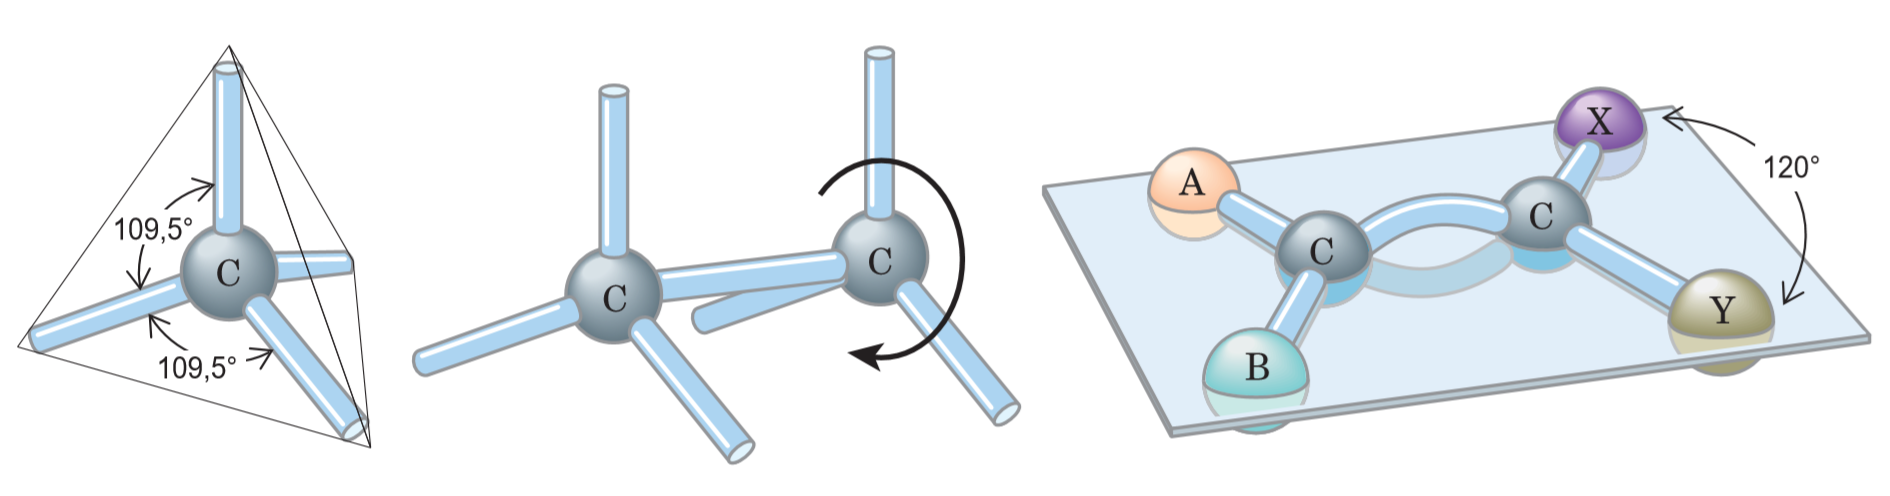
\includegraphics[width=1\linewidth]{secProteins/figures/carbono.png}
	\end{center}
	\caption{Geometria da ligação do carbono.}
	\label{fig:carbono}
\end{figure}

A versatilidade das ligações covalentes do carbono podem formar cadeias lineares, ramificadas e estruturas cíclicas. Nenhum outro elemento químico consegue formar moléculas com tanta diversidade de tamanhos, formas e composição.

\section*{Classificação Macromolecular}
As células contém um conjunto universal de moléculas pequenas. Mas como podemos discutir sobre o que é uma molécula pequena? Devemos definir uma forma de comparar os tamanhos moleculares. Na literatura existem duas medidas principais para esse fim, com uma relação bem definida entre si, tratam-se do \textit{peso molecular} (ou \textit{massa molecular relativa}), denominado $M_r$ e da \textit{massa molecular}, denotada simplesmente por $m$.

O peso molecular é definido como uma relação direta da massa da molécula da substância estudada com um duodécimo da massa do carbono-12 ($^{12}C$, em torno de $1,9926\times 10^{-23}$ gramas), note que, como $M_r$ é uma razão, não possui dimensão associada. Já a massa molecular é apenas a massa da molécula (ou massa molar) sobre o número de Avogadro --- que é definida como sendo o número de átomos por mol de uma determinada substância. Esta, diferente da massa molecular relativa, possui dimensão e é expressa em dáltons (abreviado Da) e um dálton equivale a um duodécimo da massa do carbono-12 --- donde deduze-se facilmente a relação entre massa molecular e peso molecular.

Os organismos vivos são constituídos por moléculas de características muito diversas. Existe uma coleção de aproximadamente mil moléculas consideradas pequenas ($M_r$ ${\sim}100$ a ${\sim}500$) diferentes dissolvidas na fase aquosa das células \cite{bioquimicaLehninger}. Nessa coleção está contido os aminoácidos comuns, nucleotídeos, açúcares e seus derivados fosforilados e ácidos mono, di e tricarboxílicos. Porém, neste estudo, estaremos mais preocupados com moléculas significativamente maiores, chamadas \textit{macromoléculas}.
\subsection*{Macromoléculas}
As macromoléculas são as principais constituintes das células. São polímeros\footnote[1]{Polímeros são moléculas formadas a partir de repetições de unidades estruturais menores, chamadas \textit{meros} ou \textit{monômeros}. Daí o nome, poli-meros $\approx$ vários-meros.} com peso molecular acima de ${\sim}5.000$. Polímeros menores são chamados de \textit{oligômeros} --- do grego, ``oligos'' significa ``pouco''. Proteínas (principal molécula do nosso estudo), ácidos nucleicos (DNA, RNA) e polissacarídeos são macromoléculas feitas de monômeros cujos pesos moleculares são de 500 ou menos, porém, como apresentam um grande número dessas subunidades, possuem um alto peso molecular --- até 1 milhão para proteínas e até vários bilhões para ácidos nucleicos. A síntese de macromoléculas é a atividade mais custosa energeticamente das células.

Tanto as proteínas quanto os ácidos nucleicos são polímeros lineares (isto é, que não possuem ramos ligados as suas cadeias principais, agindo como um longo fio contínuo) feitos de subunidades monoméricas bem mais simples, donde esta sequência específica de meros é que dá as informações sobre a sua estrutura tridimensional e suas funções biológicas associadas \cite{bioquimicaLehninger}.

Em especial, as proteínas são constituídas por um conjunto de monômeros muito bem conhecidos e catalogados, chamados \textit{aminoácidos}. As proteínas constituem a segunda maior fração da célula, só perdendo para a água. Provavelmente são as mais versáteis de todas as biomoléculas: Algumas tem atividade catalítica e funcionam como enzimas, outras servem como elementos estruturais, receptoras de sinais, ou transportadoras que carregam substâncias específicas para dentro ou fora das células.  

\section*{Configuração Molecular}
No mundo biomolecular, toda a informação sobre uma molécula é dada pela sua estrutura (também chamada de \textit{estereoquímica}), logo, suas ligações covalentes e seus grupos funcionais (subestruturas padrões associadas) são trivialmente importantes para definir seu bom funcionamento. Devido a característica rotacional das ligações simples do carbono, existem muitas moléculas (chamadas \textit{estereoisômeros}) com a mesma fórmula molecular e ligações químicas, mas com diferentes configurações espaciais, o que pode mudar completamente suas funções. 

De maneira simples, podemos identificar estereoisômeros pelo fato de que eles possuem as mesmas propriedades químicas, porém, não podem ser convertidos entre si sem que haja a quebra de uma ou mais ligações covalentes. Isto se dá pela presença de ligações duplas (devido a limitação na sua rotação) ou pela presença de \textit{centros quirais}, onde a molécula rotacionada não pode corresponder a sua imagem especular (conforme Figura ~\ref{fig:quiral}, extraída de \cite{bioquimicaLehninger}). Um átomo de carbono com quatro ligações diferentes é considerado assimétrico e é chamado de centro quiral --- do grego, \textit{chiros} quer dizer "mão", parafraseando estas estruturas com a relação da mão direita com a esquerda. Logo, se existir um centro quiral, sempre haverá pelo menos duas possibilidades para configuração.

\begin{figure}[H]
	\begin{center}
		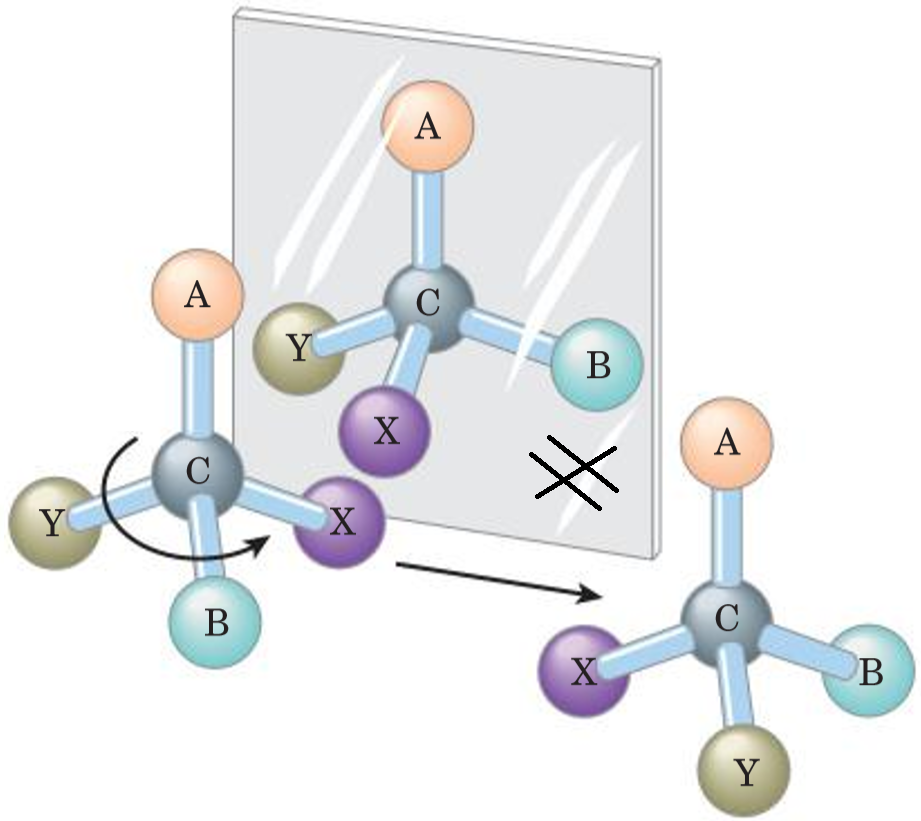
\includegraphics[width=0.45\linewidth]{secProteins/figures/quiral.png}
	\end{center}
	\caption{Ilustração de uma molécula quiral.}
	\label{fig:quiral}
\end{figure} 

Outro conceito que nos será importante no futuro, a \textit{conformação molecular} é a disposição dos átomos no espaço que pode ser mudada por rotação em torno de ligações simples, sem quebrar ligações covalentes. Estes ângulos possíveis tem posições mais estáveis e instáveis do ponto de vista energético, conforme mostra o gráfico da Figura ~\ref{fig:carener}. Podemos tentar descobrir a conformação mais provável de uma molécula minimizando a somatória de todas as forças atuantes na molécula \cite{carlileTese}. 

\begin{figure}[H]
	\begin{center}
		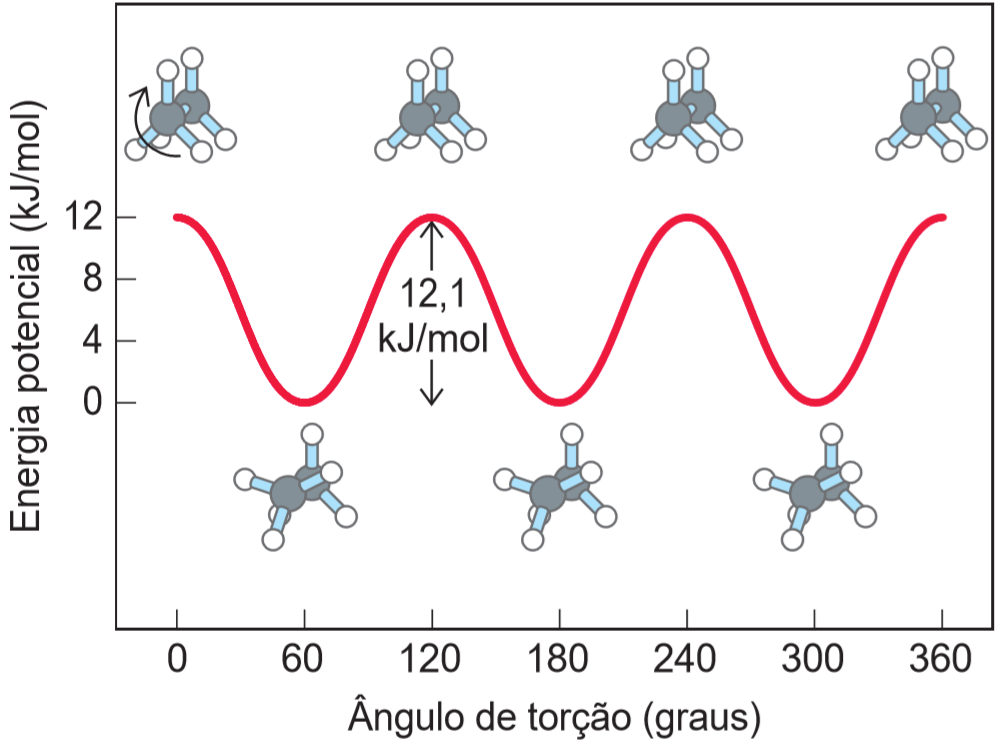
\includegraphics[width=0.55\linewidth]{secProteins/figures/carbonoenergia.png}
	\end{center}
	\caption{Conformações e Equilíbrio de Energia \cite{bioquimicaLehninger}.}
	\label{fig:carener}
\end{figure} 

Para compreender melhor como serão as configurações das moléculas que trataremos nesse texto (proteínas), vale nos preocuparmos com as subestruturas do qual eles são formados. 

\section*{Aminoácidos}
As proteínas são longas cadeias lineares de aminoácidos ligados por um tipo específico de ligação (chamada \textit{peptídica}), a qual é característica por ter como resíduo uma molécula de água. São vinte tipos diferentes de aminoácidos encontrados normalmente na natureza, sendo esses muito bem conhecidos e catalogados. O primeiro a ser descoberto foi a asparagina, em 1806; o ultimo foi a treonina, descoberto em 1938 \cite{bioquimicaLehninger}. Vale mencionar que, além destes vinte aminoácidos mais comuns, há vários outros menos frequentes, porém não constituem as proteínas.

Destes vinte aminoácidos comuns (disponíveis no Apêndice C), dezenove compartilham da mesma estrutura principal \cite{fidalgotese} --- estes são chamados $\alpha$-aminoácidos. Eles tem um grupo carboxílico e um grupo amina ligados ao mesmo átomo de carbono (o carbono $\alpha$), além de mais um hidrogênio (chamado hidrogênio $\alpha$) e, em sua última ligação, uma cadeia R que é o que diferencia cada aminoácido. Essa estrutura é ilustrada na Figura ~\ref{fig:amino}. O único aminoácido que difere disso é a Prolina, que possui como cadeia R um anel aromático que se fecha no nitrogênio (que no padrão mencionado há um grupo amina).

\begin{figure}[H]
	\begin{center}
		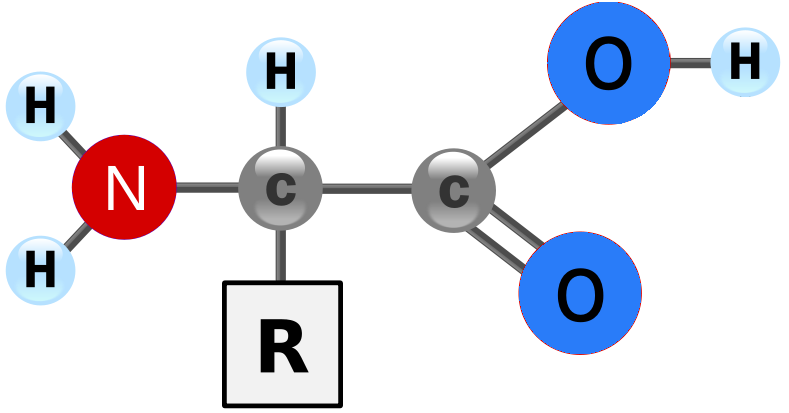
\includegraphics[width=0.35\linewidth]{secProteins/figures/amino.png}
	\end{center}
	\caption{Estrutura padrão de um $\alpha$-aminoácido.}
	\label{fig:amino}
\end{figure}

Portanto, há uma noção prévia de qual tipo de estrutura esperar ao analisar uma molécula de proteína. Existe uma estrutura conhecida e repetitiva para os átomos.

Para todos os aminoácidos comuns, exceto a glicina, o carbono $\alpha$ está ligado com quatro outros átomos diferentes entre si (na glicina temos R como apenas mais um hidrogênio, sendo o aminoácido mais simples), o que transforma o carbono $\alpha$ em um centro quiral. Logo, cada aminoácido (menos glicina) tem sempre dois estereoisômeros possíveis. Porém, na verdade, apenas um destes ocorrê naturalmente nas proteínas \cite{bioquimicaLehninger}.

\subsection*{Ligação Peptídica}
A ligação entre dois aminoácidos é feita de modo covalente por meio de desidratação do grupo $\alpha$-carboxílico de um com o grupo $\alpha$-amina do outro --- ou seja, ligar o carbono final de um no nitrogênio inicial do outro, liberando um oxigênio e dois hidrogênios, que formam uma molécula de água. Essa ligação, também chamada de resíduo (devido a liberação da água), forma um dipeptídeo. 

Quando muitos aminoácidos se juntam, o produto é chamado de polipeptídeo. Perceba que os termos ``polipeptídeo'' e ``proteína'' parecem dirigir-se as mesmas moléculas, porém, a diferença está na massa molecular: As moléculas com massa abaixo de 10.000 são ditas polipeptídeos, enquanto as maiores que essas são consideradas proteínas. Os comprimentos dessas cadeias variam significativamente. O citocromo c humano tem apenas 104 aminoácidos, enquanto, no outro extremo, a titina (relacionada ao músculo de vertebrados) possui aproximadamente 27.000 aminoácidos e uma massa molecular de cerca de 3.000.000. No geral, as proteínas naturais contém menos de 2.000 aminoácidos \cite{bioquimicaLehninger}.

Outra característica muito importante das ligações peptídicas é de que elas se comportam semelhantemente a ligações covalentes duplas dos carbonos. Estudos envolvendo difração de raios X em cristais de aminoácidos e polipeptídeos descobriram que a ligação peptídica $C-N$ é de alguma forma mais curta que a ligação de uma amina simples, e que os átomos associados a ligação peptídica estão todos co-planares (conforme Figura ~\ref{fig:peptidica}). Perceba que também são rígidos, não sendo possível a rotação. Essa é uma propriedade muito útil que também nos será importante, descoberta de 1930 que se deve a Linus Pauling e Robert Corey.

\begin{figure}[H]
	\begin{center}
		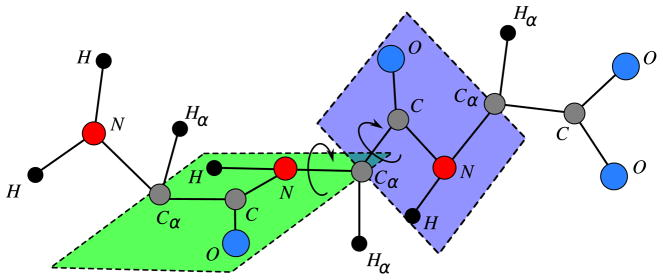
\includegraphics[width=0.8\linewidth]{secProteins/figures/peptide.jpg}
	\end{center}
	\caption{O grupo peptídico planar \cite{carlile:MinimalOrder}.}
	\label{fig:peptidica}
\end{figure}

\section*{Estrutura das Proteínas}
A estrutura de proteínas pode ser descrita em quatro níveis de importante hierarquia conceitual, conforme pode ser visto na Figura ~\ref{fig:protest}, retirado de \cite{bioquimicaLehninger}. A estrutura primaria consiste da mais detalhada, sendo de fato os polímeros de aminoácidos; Estes, por sua vez, formam alguns arranjos particularmente estáveis, que dão origem a padrões estruturais recorrentes, que chamamos de \textit{estruturas secundárias} (como as hélices $\alpha$, as duplas hélices etc..). A estrutura terciária descreve todos os aspectos do enovelamento tridimensional de um polipeptídeo, ou seja, define quais serão as forças atuantes na molécula --- que da origem a sua conformação estável, que minimiza a energia livre de Gibbs do sistema. Quando existem mais estruturas terciárias em uma proteína, chamamos a junção destas de estrutura quaternária.	

\begin{figure}[H]
	\begin{center}
		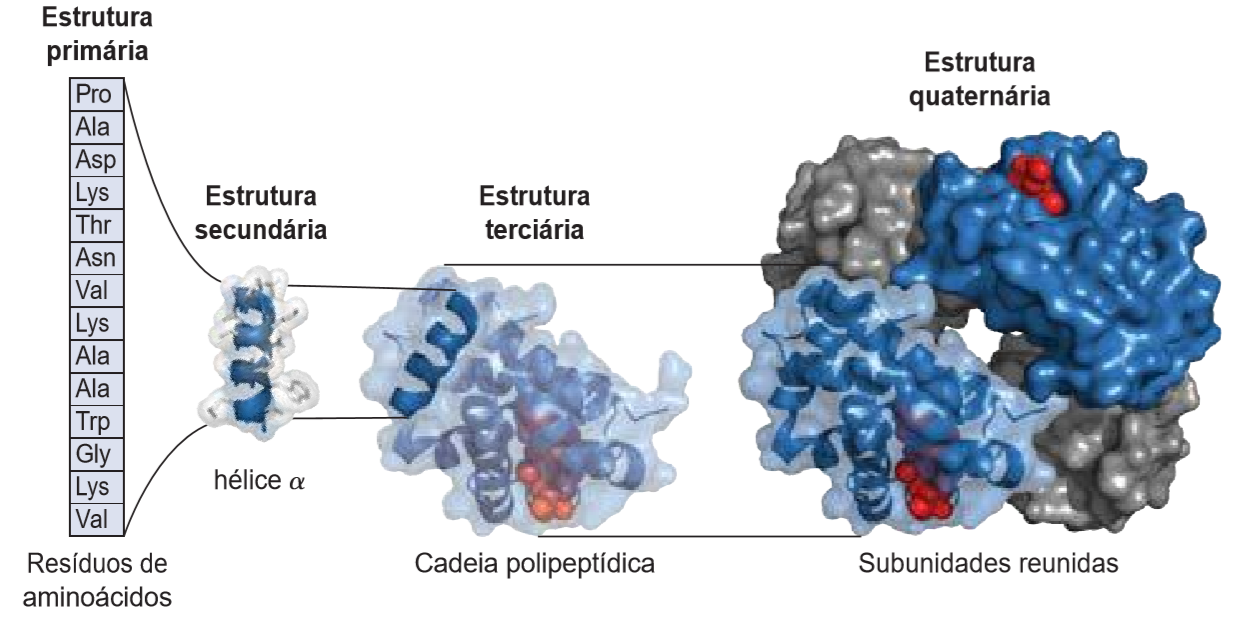
\includegraphics[width=0.9\linewidth]{secProteins/figures/protest.png}
	\end{center}
	\caption{Níveis de estrutura das proteínas exemplificados na Hemoglobina.}
	\label{fig:protest}
\end{figure}

Em especial, as diferentes configurações da estrutura primária --- que pode mudar drasticamente entre estruturas primárias diferentes na mesma molécula --- nos é mais informativa. A estrutura primária de uma proteína determina como ela se dobra em sua estrutura tridimensional, devido os ângulos e distâncias bem definidos de suas ligações entre átomos, que da a sua estrutura especial; o que, por sua vez, determina a função da proteína --- como no exemplo da Figura ~\ref{fig:protest}, onde a estrutura da hemoglobina é que permite que átomos de oxigênio ``encaixem'' nela, possibilitando o transporte desse átomo pelo organismo, que é sua função (e só o é dado sua estrutura tridimensional). 

Por sua relação com a estrutura tridimensional e, logo, função das proteínas, vamos nos concentrar em estudar a subdivisão de estruturas primárias. 

\subsection*{A Cadeia Principal de uma Proteína}
Quando se estuda proteínas a nível dos aminoácidos, não tardamos a perceber que elas possuem uma estrutura repetida muito interessante do ponto de vista bioquímico. Trata-se da \textit{cadeia principal} de uma proteína, também chamada de \textit{Backbone} --- espinha dorsal, em tradução literal, fazendo alusão a importância desta estrutura. Perceba que os vinte aminoácidos que compõem as proteínas possuem sempre os mesmos três átomos ligados em sequência (Figura ~\ref{fig:backbone}): $N-C_\alpha-C$, através de ligações covalentes em torno do $C_\alpha$ e da ligação peptídica $C-N$ entre aminoácidos.

\begin{figure}[H]
	\begin{center}
		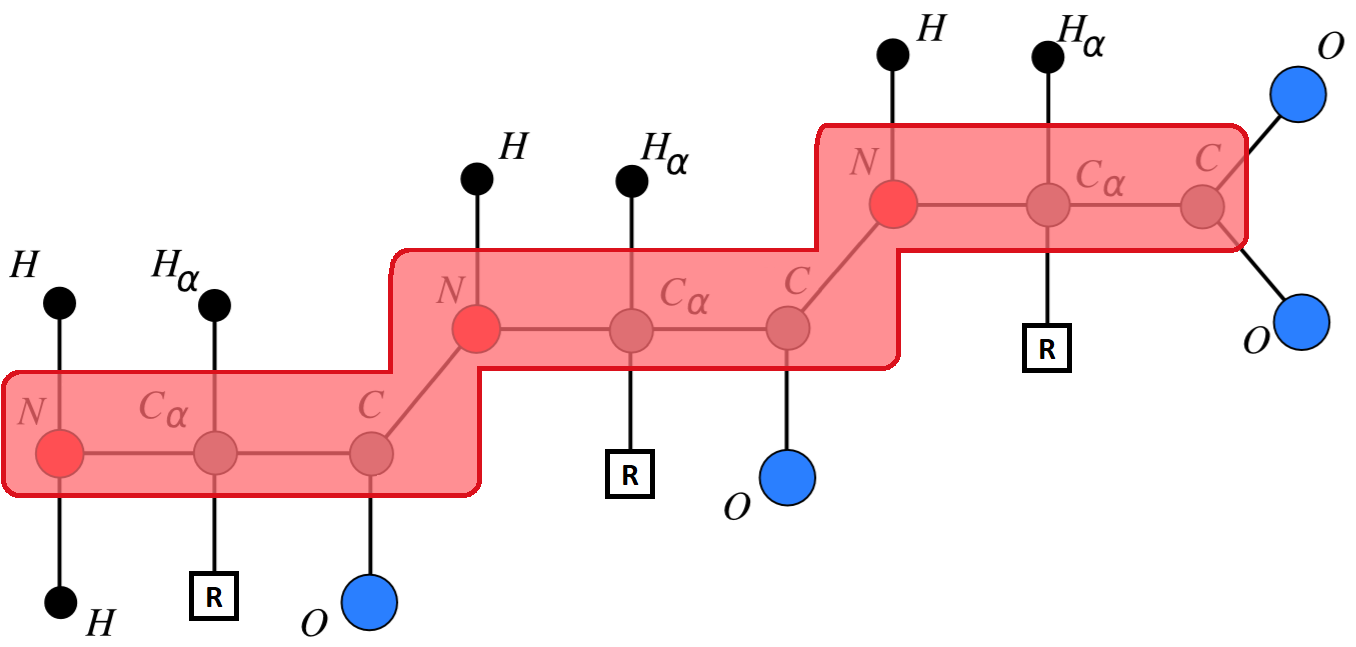
\includegraphics[width=0.8\linewidth]{secProteins/figures/backbone.png}
	\end{center}
	\caption{Representação da cadeia principal da proteína, adaptada de  \cite{carlile:MinimalOrder}}.
	\label{fig:backbone}
\end{figure}

Outra informação bastante útil sobre esta cadeia principal é que, devido dados experimentais de cristalografia, sabe-se sobre a geometria média dessa subestrutura \cite{ramachandran1974MolStructure}, onde os comprimentos e ângulos entre  as ligações dos átomos que a formam são fixas, na média, a menos de erros de medida. Vide Figura ~\ref{fig:rama}, extraída do texto original de Ramachandran \textit{et al}, um dos precursores deste estudo.

\begin{figure}[H]
	\begin{center}
		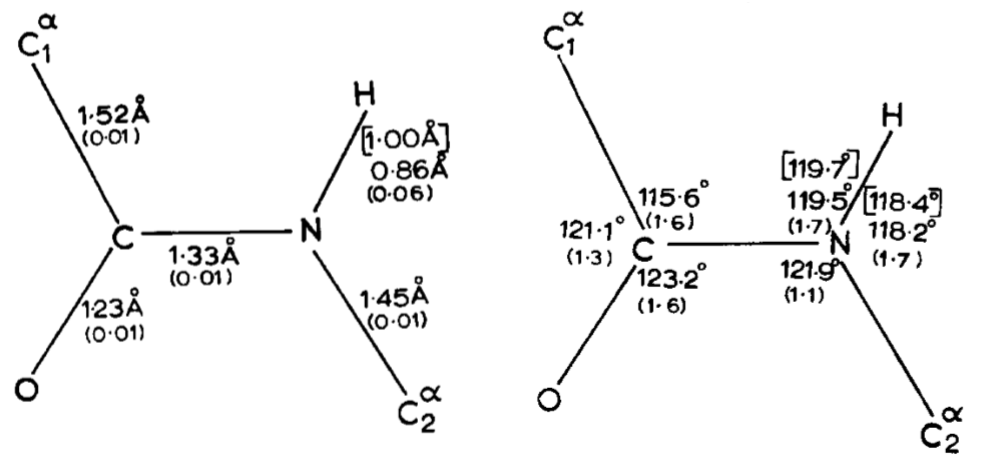
\includegraphics[width=0.8\linewidth]{secProteins/figures/rama.png}
	\end{center}
	\caption{Dados de ângulos e distâncias médios de ligações em um aminoácido.}
	\label{fig:rama}
\end{figure}


\section*{\textit{Worldwide Protein Data Bank}}
Já foi possível perceber a grande variedade de diferentes configurações possíveis para as proteínas. Com isso, há a necessidade de se estudar cada uma explicitamente, através de experimentos, catalogando e guardando essas informações. Esse grande esforço para entender o mundo das macromoléculas se deixa transparecer com o repositório \textit{Worldwide Protein Data Bank} --- ou simplesmente wwPDB \cite{wwPDB}.

Este é um repositório online e público onde estão guardadas todas os dados de proteínas e ácidos nucleicos já catalogados, em especial dados de suas estruturas 3D (posições x, y e z de cada um dos átomos que a constituem). Auxiliando tanto pesquisadores, quanto professores e estudantes, essa base de dados é um grande esforço em conjunto de físicos, biólogos, bioquímicos e vários outros profissionais de diversas áreas do conhecimento de todo o mundo.

\subsection*{Arquivo PDB}
Quando se quer estudar uma proteína no repositório PDB, base fazer o \textit{download} do arquivo PDB da molécula (extensão ``.ent''). Esse é um arquivo de estruturas tridimensionais de macromoléculas biológicas determinadas experimentalmente, que descrevem as coordenadas espaciais de cada átomo cuja posição foi determinada (muitas das estruturas catalogadas não estão completas); também existem dados adicionais sobre informações de como as estruturas foram determinadas, os dados práticos dos experimentos, a precisão associada aos dados e tudo mais que quem estiver criando o documento achar necessário para aquela macromolécula.

Tecnicamente, o arquivo PDB trata-se de uma representação estruturada dos dados moleculares e experimentais da proteína. Ele é separado por seções, onde cada seção pode possuir subseções. São elas: 
\begin{itemize}
	\item \textbf{Seção Title} - Contem a descrição da molécula;
	\vspace{-0.3cm}
	
	\item \textbf{Seção Remark} - Vários comentários sobre anotações de entrada com mais profundidade que os registros padrões;
	\vspace{-0.3cm}
	
	\item \textbf{Seção Primary structure} - Sequências peptídicas ou nucleotídicas especificadas para serem posteriormente utilizadas, diminuindo a repetição do arquivo;
	
	\vspace{-0.3cm}
	\item \textbf{Seção Heterogen} - Descrição de grupos presentes não padronizados --- Visto que proteínas também podem conter materiais inorgânicos, como o ferro presente na hemoglobina (vide Figura ~\ref{fig:protest});
	\vspace{-0.3cm}
	
	\item \textbf{Seção Secondary structure} - Descrição das estruturas secundárias presentes na molécula;
	
	\vspace{-0.3cm}
	\item \textbf{Seção Connectivity annotation} - Descrição das conectividade químicas da molécula;
	\vspace{-0.3cm}
	
	\item \textbf{Seção Miscellaneous features} - Descrição dos recursos dentro da macromolécula;
	\vspace{-0.3cm}
	
	\item \textbf{Seção Crystallographic} - Descrição de parâmetros da cristalografia, quando o experimento utiliza esta metodologia;
	
	\vspace{-0.3cm}
	\item \textbf{Seção Coordinate transformation} - Matrizes como operadores de transformação das coordenadas;
	\vspace{-0.3cm}
	
	\item \textbf{Seção Coordinate} - Dados de coordenadas atômicas, a seção que mais vamos utilizar;
	\vspace{-0.3cm}
	
	\item \textbf{Seção Connectivity} - Citação das conexões químicas entre os átomos;
	\vspace{-0.3cm}
	
	\item \textbf{Seção Bookkeeping} - Resumo das características totais do arquivo e o marcador de fim de arquivo.
\end{itemize}

Como o arquivo é significativamente extenso, não entraremos em detalhes neste texto sobre as características detalhadas de cada uma das seções apresentadas. Porém, vale mencionar o tipo de entrada ATOM, presente na seção Coordinate, pois essa é a entrada que compõe a maior parte dos arquivos PDB, além de ser a de nosso interesse principal.

A entrada ATOM tem como objetivo descrever detalhes de cada átomo específico da molécula. Ela segue um padrão indentado, onde cada dado é caracterizado pela sua posição na linha (coluna). Segue principais dados da entrada e suas respectivas colunas na Tabela ~\ref{table:atom}.

\begin{table}[h!]
	\centering
	\begin{tabular}{ |c|c| } 
		\hline
		Código serial do átomo & 7-11 \\ 
		\hline
		Nome do átomo & 13-16 \\ 
		\hline
		Nome do resíduo que pertence & 18-20 \\ 
		\hline
		Identificador da cadeia & 22 \\ 
		\hline
		Código serial de dentro do resíduo & 23-26 \\ 
		\hline
		Coordenada x & 31-38 \\ 
		\hline
		Coordenada y & 39-46 \\ 
		\hline
		Coordenada z & 47-54 \\ 
		\hline
		\textit{Occupancy} do átomo & 55-60 \\ 
		\hline
		Fator de temperatura & 61-66 \\ 
		\hline
		Simbolo do elemento & 77-78 \\
		\hline
	\end{tabular}
	\caption{Principais dados da entrada ATOM.}
	\label{table:atom}
\end{table}

\vspace{-0.4cm}
Segue exemplo de um conjunto de entradas do tipo ATOM na Figura ~\ref{fig:atom}.
\begin{figure}[H]
	\begin{center}
		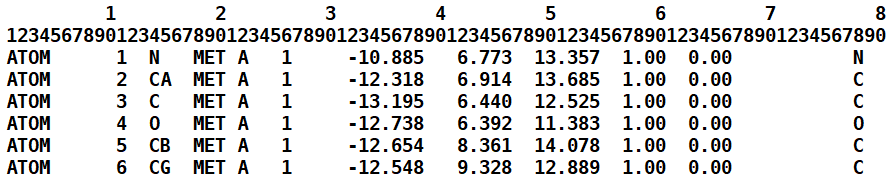
\includegraphics[width=0.95\linewidth]{secProteins/figures/atom.png}
	\end{center}
	\caption{Conjunto de entradas do tipo ATOM.}
	\label{fig:atom}
\end{figure}
\vspace{-0.3cm}

Com esse conjunto de dados, pode-se, por exemplo, esboçar uma representação gráfica de uma molécula. Existem muitos softwares compatíveis com os arquivos PDB para este fim, por exemplo, o autor deste documento implementou uma visualização de uma projeção da molécula 3D no plano z = 0, como pode-se averiguar na Figura~\ref{fig:molproj}.

\begin{figure}[H]
	\begin{center}
		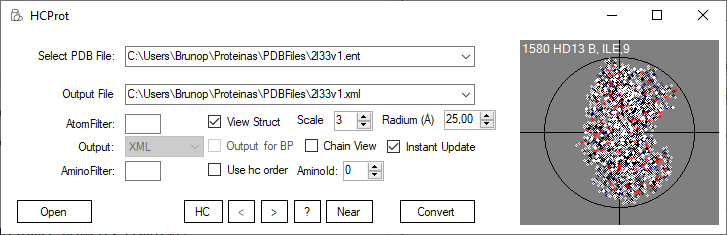
\includegraphics[width=1\linewidth]{secProteins/figures/molproj.png}
	\end{center}
	\caption{HCProt com visualização a partir de um aquivo PDB.}
	\label{fig:molproj}
\end{figure}

\chapter{Vinte Aminoácidos Naturais} 

É comum dividirmos os aminoácidos proteicos em cinco classes, como segue.
\subsubsection*{Grupos R apolares, alifáticos}
\begin{figure}[H]
	\begin{center}
		\begin{minipage}{0.24\linewidth}
			\centering   
			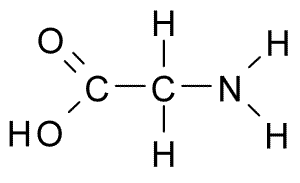
\includegraphics[width=0.95\linewidth]{secProteins/figures/glycine.png}	
			\caption{Glicina}
			\label{fig:glycine}
		\end{minipage}
		\begin{minipage}{0.24\linewidth}
			\centering   
			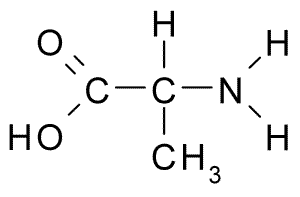
\includegraphics[width=0.9\linewidth]{secProteins/figures/alanine.png}
			\caption{Alanina}
			\label{fig:alanine}
		\end{minipage}
		\begin{minipage}{0.24\linewidth}
			\centering   
			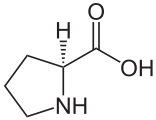
\includegraphics[width=0.8\linewidth]{secProteins/figures/proline.png}
			\caption{Prolina}
			\label{fig:proline}
		\end{minipage}
		\begin{minipage}{0.24\linewidth}
			\centering   
			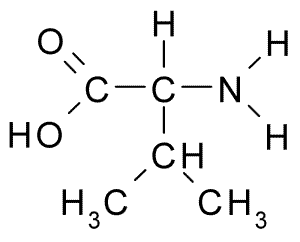
\includegraphics[width=0.8\linewidth]{secProteins/figures/valine.png}
			\caption{Valina}
			\label{fig:valine}
		\end{minipage}
	\end{center}
\end{figure}
\vspace{-1cm}
\begin{figure}[H]
	\begin{center}
		\begin{minipage}{0.3\linewidth}
			\centering   
			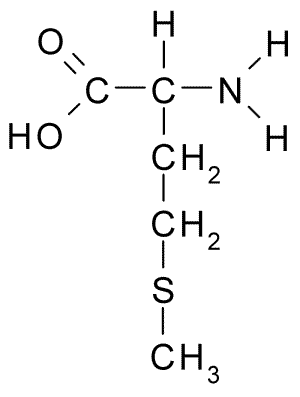
\includegraphics[width=0.63\linewidth]{secProteins/figures/methionine.png}	
			\caption{Metionina}
			\label{fig:methionine}
		\end{minipage}
		\begin{minipage}{0.3\linewidth}
			\centering   
			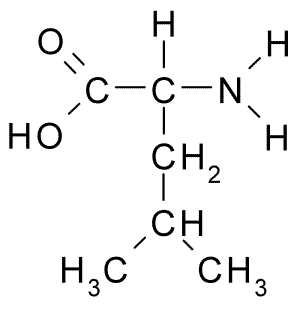
\includegraphics[width=0.8\linewidth]{secProteins/figures/leucine.png}
			\caption{Leucina}
			\label{fig:leucine}
		\end{minipage}
		\begin{minipage}{0.3\linewidth}
			\centering   
			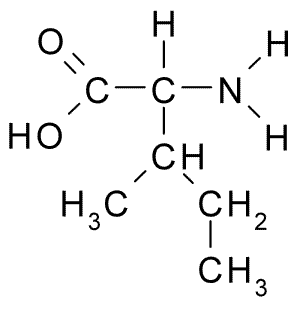
\includegraphics[width=0.8\linewidth]{secProteins/figures/isoleucine.png}
			\caption{Isoleucina}
			\label{fig:isoleucine}
		\end{minipage}
	\end{center}
\end{figure}

\subsubsection*{Grupos R polares, não carregados}	

\begin{figure}[H]
	\begin{center}
		\begin{minipage}{0.3\linewidth}
			\centering   
			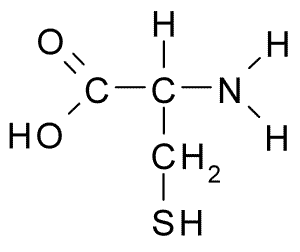
\includegraphics[width=0.8\linewidth]{secProteins/figures/cysteine.png}	
			\caption{Cisteína}
			\label{fig:cysteine}
		\end{minipage}
		\begin{minipage}{0.3\linewidth}
			\centering   
			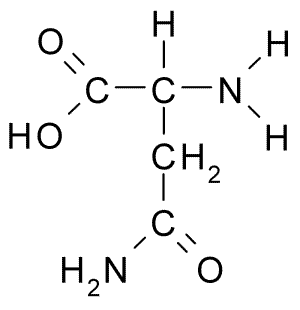
\includegraphics[width=0.65\linewidth]{secProteins/figures/asparagine.png}
			\caption{Asparagina}
			\label{fig:asparagine}
		\end{minipage}
		\begin{minipage}{0.3\linewidth}
			\centering   
			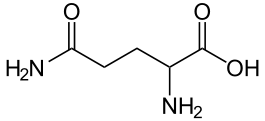
\includegraphics[width=1\linewidth]{secProteins/figures/glutamine.png}
			\caption{Glutamina}
			\label{fig:glutamine}
		\end{minipage}
	\end{center}
\end{figure}
\vspace{-1cm}
\begin{figure}[H]
	\begin{center}
		\begin{minipage}{0.45\linewidth}
			\centering   
			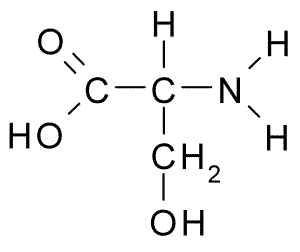
\includegraphics[width=0.5\linewidth]{secProteins/figures/serine.png}	
			\caption{Serina}
			\label{fig:serine}
		\end{minipage}
		\begin{minipage}{0.45\linewidth}
			\centering   
			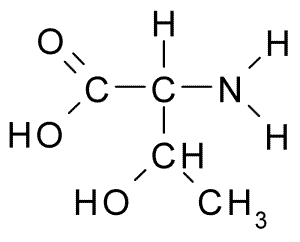
\includegraphics[width=0.5\linewidth]{secProteins/figures/threonine.png}
			\caption{Treonina}
			\label{fig:threonine}
		\end{minipage}
	\end{center}
\end{figure}

\subsubsection*{Grupos R aromáticos}
\begin{figure}[H]
	\begin{center}
		\begin{minipage}{0.3\linewidth}
			\centering   
			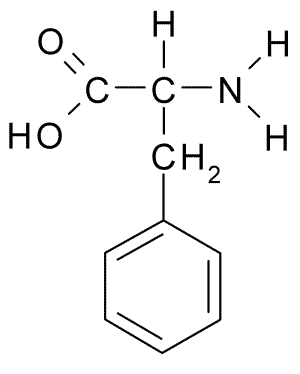
\includegraphics[width=0.7\linewidth]{secProteins/figures/phenylalanine.png}	
			\caption{Fenilalanina}
			\label{fig:phenylalanine}
		\end{minipage}
		\begin{minipage}{0.3\linewidth}
			\centering   
			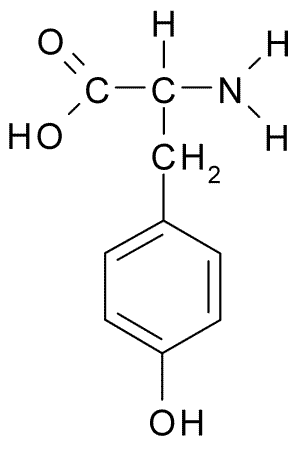
\includegraphics[width=0.59\linewidth]{secProteins/figures/tyrosine.png}
			\caption{Tirosina}
			\label{fig:tyrosine}
		\end{minipage}
		\begin{minipage}{0.3\linewidth}
			\centering   
			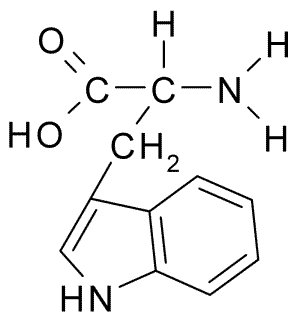
\includegraphics[width=0.7\linewidth]{secProteins/figures/tryptophan.png}
			\caption{Triptofano}
			\label{fig:tryptophan}
		\end{minipage}
	\end{center}
\end{figure}

\subsubsection*{Grupos R carregados positivamente}
\begin{figure}[H]
	\begin{center}
		\begin{minipage}{0.3\linewidth}
			\centering   
			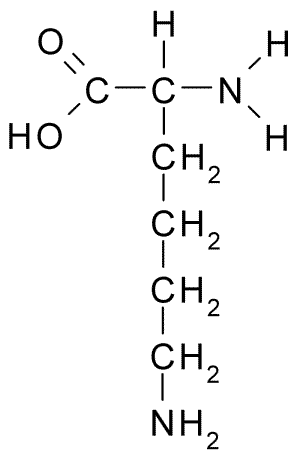
\includegraphics[width=0.7\linewidth]{secProteins/figures/lysine.png}	
			\caption{Lisina}
			\label{fig:lysine}
		\end{minipage}
		\begin{minipage}{0.3\linewidth}
			\centering   
			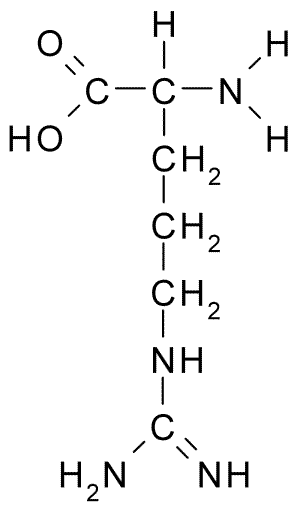
\includegraphics[width=0.59\linewidth]{secProteins/figures/arginine.png}
			\caption{Arginina}
			\label{fig:arginine}
		\end{minipage}
		\begin{minipage}{0.3\linewidth}
			\centering   
			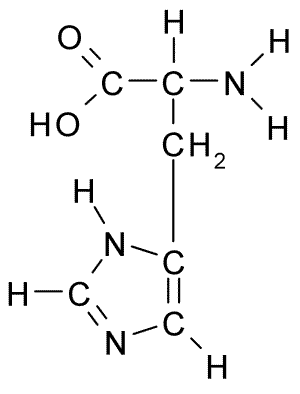
\includegraphics[width=0.7\linewidth]{secProteins/figures/histidine.png}
			\caption{Histidina}
			\label{fig:histidine}
		\end{minipage}
	\end{center}
\end{figure}

\subsubsection*{Grupos R carregados negativamente}

\begin{figure}[H]
	\begin{center}
		\begin{minipage}{0.45\linewidth}
			\centering   
			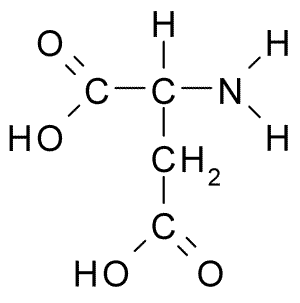
\includegraphics[width=0.5\linewidth]{secProteins/figures/asparticacid.png}	
			\caption{Aspartato}
			\label{fig:asparticacid}
		\end{minipage}
		\begin{minipage}{0.45\linewidth}
			\centering   
			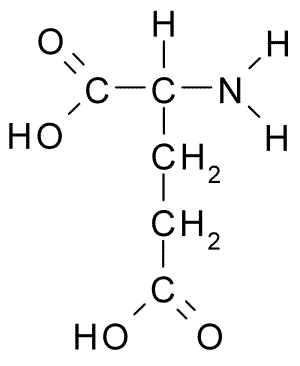
\includegraphics[width=0.45\linewidth]{secProteins/figures/glutamicacid.png}
			\caption{Glutamato}
			\label{fig:glutamicacid}
		\end{minipage}
	\end{center}
\end{figure}

	
	\chapter{Tabelas de Simulações Computacionais\label{ap:tabelas}}
	No que se segue, há duas extensas tabelas com os resultados computacionais gerais e de operações das simulações de cada proteína no banco de testes (identificada pelo seu código PDB na primeira coluna).
	
	\begin{footnotesize}
		\begin{xltabular}{\textwidth}{||rS[table-format=1.3e+2]S[table-format=1.4e+2]S[table-format=1.4e+2]||}
		\caption{Resultados gerais} \label{tab:genResults}\\
		\toprule
		\multicolumn{1}{||c}{Problema} & \multicolumn{1}{c}{LDE} & \multicolumn{1}{c}{RMSD} & \multicolumn{1}{c||}{Tempo} \\
		\midrule
		\endfirsthead
		\caption{Resultados gerais - continuação}\\
		\toprule
		\multicolumn{1}{||c}{Problema} & \multicolumn{1}{c}{LDE} & \multicolumn{1}{c}{RMSD} & \multicolumn{1}{c||}{Tempo} \\
		\midrule
		\endhead
pdb1ba5 & 4.257e-21 & 1.8249e-10 & 1.5480e-01 \\
pdb1d1n & 4.268e-11 & 1.1200e-11 & 4.3957e-01 \\
pdb1dp3 & 2.048e-10 & 8.2794e-11 & 3.4111e-01 \\
pdb1du1 & 2.921e-21 & 1.1862e-12 & 2.2095e-02 \\
pdb1fcl & 1.650e-10 & 2.5527e-12 & 5.0979e-01 \\
pdb1fd6 & 3.248e-20 & 1.4000e-11 & 2.9719e-01 \\
pdb1i2u & 4.779e-22 & 9.1058e-12 & 9.5673e-02 \\
pdb1i2v & 3.179e-22 & 9.5660e-13 & 1.3251e-01 \\
pdb1jlz & 3.852e-22 & 8.6556e-12 & 2.9969e-02 \\
pdb1k0v & 8.541e-23 & 3.0991e-13 & 2.3770e-01 \\
pdb1k37 & 6.716e-22 & 6.5474e-13 & 3.0247e-01 \\
pdb1kuw & 8.201e-24 & 6.6737e-13 & 7.4609e-03 \\
pdb1kz0 & 2.722e-24 & 6.9116e-13 & 1.5744e-02 \\
pdb1kz2 & 4.694e-25 & 4.2483e-12 & 1.7705e-02 \\
pdb1kz5 & 2.280e-24 & 2.9273e-12 & 1.0726e-02 \\
pdb1lvz & 2.004e-10 & 6.6194e-13 & 7.5792e-03 \\
pdb1m4e & 1.304e-10 & 5.9826e-12 & 2.1013e-02 \\
pdb1ma2 & 8.239e-10 & 4.8491e-11 & 2.0457e-01 \\
pdb1ma4 & 1.637e-10 & 5.5679e-13 & 6.6045e-02 \\
pdb1ma5 & 7.238e-22 & 4.1675e-12 & 1.6453e-02 \\
pdb1ma6 & 3.569e-11 & 6.0995e-11 & 1.7111e-02 \\
pdb1nd9 & 2.343e-22 & 1.8713e-12 & 3.6278e-01 \\
pdb1ne5 & 3.682e-21 & 9.1988e-12 & 1.9038e-01 \\
pdb1nmj & 1.380e-25 & 1.6907e-13 & 4.0840e-02 \\
pdb1o53 & 1.022e-10 & 1.1873e-12 & 1.5900e-02 \\
pdb1plw & 5.299e-25 & 4.6242e-13 & 2.4468e-03 \\
pdb1plx & 5.592e-24 & 4.7012e-12 & 2.2908e-03 \\
pdb1pv0 & 1.232e-10 & 3.3931e-12 & 1.3642e-01 \\
pdb1r57 & 1.769e-12 & 2.1316e-12 & 7.0222e-01 \\
pdb1ry3 & 2.466e-10 & 3.4230e-12 & 2.3248e-01 \\
pdb1s4h & 8.707e-13 & 8.7429e-12 & 1.0301e-02 \\
pdb1s4j & 3.470e-10 & 9.2762e-13 & 1.1796e-02 \\
pdb1sa8 & 7.551e-21 & 2.7989e-12 & 5.2512e-01 \\
pdb1t2y & 6.970e-23 & 2.7851e-12 & 3.8073e-02 \\
pdb1t5q & 1.372e-24 & 1.4825e-13 & 4.2397e-02 \\
pdb1tot & 9.344e-24 & 2.3697e-13 & 1.2389e-01 \\
pdb1v6r & 1.378e-21 & 3.7304e-12 & 2.6783e-02 \\
pdb1v92 & 2.846e-23 & 2.4804e-12 & 1.0928e-01 \\
pdb1vd7 & 2.704e-10 & 2.3012e-12 & 2.8572e-02 \\
pdb1vd9 & 1.193e-09 & 3.8355e-11 & 3.3708e-02 \\
pdb1vdb & 4.944e-10 & 1.1210e-11 & 2.8438e-02 \\
pdb1vpc & 1.105e-25 & 1.0206e-13 & 9.1858e-02 \\
pdb1wnk & 6.740e-20 & 7.6026e-10 & 2.8723e-02 \\
pdb1wo4 & 3.313e-21 & 1.3690e-11 & 2.4109e-01 \\
pdb1wo5 & 4.597e-11 & 1.6851e-11 & 6.2035e-02 \\
pdb1y5c & 4.251e-11 & 9.7008e-12 & 8.7486e-03 \\
pdb1yxr & 2.219e-11 & 2.3743e-12 & 5.5868e-01 \\
pdb2a4j & 4.366e-24 & 2.9037e-13 & 4.8866e-01 \\
pdb2ajj & 3.438e-10 & 1.1290e-12 & 4.5503e-02 \\
pdb2ajm & 2.889e-10 & 3.0199e-12 & 4.5681e-02 \\
pdb2ajn & 1.802e-10 & 4.6193e-13 & 4.4141e-02 \\
pdb2ajo & 2.889e-10 & 3.0199e-12 & 4.7050e-02 \\
pdb2akk & 2.487e-23 & 1.1166e-12 & 6.8753e-01 \\
pdb2c0s & 6.254e-22 & 1.3872e-11 & 1.8404e-01 \\
pdb2dci & 5.202e-25 & 1.0732e-13 & 2.2076e-02 \\
pdb2eem & 1.553e-21 & 7.6795e-12 & 1.4027e-01 \\
pdb2fxz & 8.123e-10 & 4.9386e-12 & 1.1497e-02 \\
pdb2g9l & 5.977e-24 & 1.9157e-12 & 7.1706e-02 \\
pdb2h5m & 3.715e-12 & 2.4650e-11 & 5.3797e-01 \\
pdb2hep & 1.788e-20 & 1.7197e-11 & 2.5101e-01 \\
pdb2jmy & 3.343e-21 & 1.2262e-12 & 1.6450e-02 \\
pdb2jn5 & 2.985e-13 & 1.1243e-11 & 1.3755e-02 \\
pdb2jpn & 1.655e-22 & 4.9731e-12 & 5.2679e-01 \\
pdb2jua & 6.900e-18 & 2.0200e-11 & 5.7446e-01 \\
pdb2jvd & 4.315e-24 & 3.6252e-13 & 1.2183e-01 \\
pdb2jws & 8.553e-11 & 1.0841e-12 & 1.6656e-01 \\
pdb2jwu & 6.308e-11 & 6.6652e-12 & 4.9427e-01 \\
pdb2jxf & 2.349e-11 & 1.2542e-12 & 4.8806e-02 \\
pdb2jz5 & 3.915e-22 & 6.3878e-13 & 7.7606e-01 \\
pdb2k2a & 2.783e-24 & 2.8282e-12 & 2.4012e-01 \\
pdb2k37 & 6.702e-23 & 2.5914e-12 & 1.8849e-01 \\
pdb2k3i & 7.168e-22 & 1.8935e-12 & 8.5926e-01 \\
pdb2kdh & 1.914e-10 & 1.2342e-09 & 3.7287e-01 \\
pdb2kdl & 5.538e-11 & 3.8154e-12 & 4.4728e-01 \\
pdb2kdm & 6.081e-11 & 7.3936e-12 & 3.0538e-01 \\
pdb2kdp & 2.725e-22 & 1.7049e-12 & 2.4970e-01 \\
pdb2kdr & 3.104e-11 & 3.3412e-13 & 4.8288e-02 \\
pdb2kes & 4.201e-24 & 3.1744e-13 & 1.4617e-01 \\
pdb2kjn & 7.890e-14 & 1.3838e-12 & 3.8902e-02 \\
pdb2kjo & 1.239e-10 & 9.3751e-12 & 3.5280e-02 \\
pdb2kl5 & 1.254e-22 & 3.1368e-12 & 6.1909e-01 \\
pdb2klz & 9.391e-25 & 4.6317e-13 & 1.2151e-01 \\
pdb2koz & 3.052e-10 & 1.6248e-11 & 6.5896e-02 \\
pdb2kp0 & 1.444e-11 & 6.2079e-11 & 2.0686e-01 \\
pdb2ksg & 9.982e-25 & 6.1641e-13 & 1.1330e-01 \\
pdb2kt8 & 4.331e-20 & 4.9046e-12 & 9.6049e-01 \\
pdb2kuh & 1.309e-24 & 7.0876e-13 & 2.1599e-01 \\
pdb2kwh & 1.274e-22 & 3.6703e-12 & 1.7506e-01 \\
pdb2kxa & 9.598e-11 & 4.1552e-12 & 2.6912e-02 \\
pdb2l3m & 2.841e-21 & 6.0669e-13 & 2.3492e-01 \\
pdb2l45 & 5.244e-25 & 1.5900e-13 & 2.9181e-02 \\
pdb2l5r & 1.046e-24 & 6.2394e-13 & 3.5440e-02 \\
pdb2l6q & 1.881e-10 & 9.8136e-10 & 5.6486e-01 \\
pdb2l6r & 4.111e-11 & 1.8748e-11 & 1.9053e-01 \\
pdb2l98 & 5.266e-22 & 3.2376e-11 & 8.7326e-01 \\
pdb2lde & 9.211e-25 & 3.3386e-13 & 3.4504e-02 \\
pdb2le7 & 3.827e-25 & 1.0978e-13 & 2.3663e-02 \\
pdb2ler & 7.513e-26 & 4.8108e-14 & 9.1923e-03 \\
pdb2lgi & 3.866e-21 & 5.4589e-12 & 3.2107e-01 \\
pdb2lhc & 1.418e-10 & 1.2994e-09 & 1.9096e-01 \\
pdb2lhe & 1.092e-17 & 6.3217e-12 & 5.6474e-01 \\
pdb2lhg & 1.904e-23 & 3.2233e-13 & 1.3247e-01 \\
pdb2lix & 5.759e-24 & 1.4715e-12 & 3.8142e-02 \\
pdb2lld & 1.197e-22 & 1.9602e-12 & 7.3642e-02 \\
pdb2lm9 & 2.575e-23 & 7.9847e-13 & 4.5876e-01 \\
pdb2lmf & 4.430e-11 & 2.3248e-12 & 2.7945e-02 \\
pdb2ln3 & 7.449e-23 & 9.4479e-14 & 3.4833e-01 \\
pdb2lo2 & 5.148e-25 & 5.0804e-13 & 7.3381e-02 \\
pdb2lqp & 1.624e-10 & 1.9702e-11 & 2.4649e-01 \\
pdb2ls9 & 2.515e-23 & 6.9713e-13 & 3.0487e-02 \\
pdb2lsa & 5.354e-24 & 3.4845e-13 & 2.9442e-02 \\
pdb2lss & 3.382e-23 & 3.6848e-12 & 2.1829e-01 \\
pdb2lt3 & 7.866e-23 & 3.4123e-13 & 5.1627e-01 \\
pdb2lu6 & 6.370e-26 & 1.9324e-14 & 1.3772e-02 \\
pdb2lwa & 1.773e-10 & 4.6809e-12 & 2.2819e-01 \\
pdb2lx0 & 6.786e-11 & 1.9476e-12 & 5.4744e-02 \\
pdb2lxz & 1.797e-20 & 8.0453e-12 & 6.3673e-01 \\
pdb2m1a & 1.720e-26 & 1.3767e-13 & 5.0159e-02 \\
pdb2m1j & 3.282e-25 & 5.4650e-13 & 5.0129e-02 \\
pdb2m2y & 1.315e-22 & 1.1427e-12 & 2.0066e-02 \\
pdb2m3f & 1.628e-24 & 3.2592e-13 & 2.7007e-02 \\
pdb2m8m & 9.789e-25 & 1.5744e-12 & 3.6070e-02 \\
pdb2m8o & 2.020e-25 & 2.0793e-13 & 3.4869e-02 \\
pdb2m97 & 1.529e-23 & 4.2576e-12 & 2.0863e-01 \\
pdb2m9r & 3.184e-24 & 1.2995e-12 & 8.8002e-02 \\
pdb2me1 & 4.660e-23 & 4.1648e-12 & 4.2620e-02 \\
pdb2me2 & 2.316e-10 & 1.8283e-12 & 3.8051e-02 \\
pdb2me3 & 1.748e-10 & 2.5263e-12 & 3.6794e-02 \\
pdb2me4 & 1.462e-10 & 9.3376e-13 & 4.3952e-02 \\
pdb2mg1 & 2.185e-24 & 1.3041e-12 & 3.2521e-02 \\
pdb2mg2 & 3.530e-25 & 1.4276e-13 & 3.4403e-02 \\
pdb2mg3 & 3.333e-24 & 8.2131e-13 & 3.6846e-02 \\
pdb2mh8 & 5.209e-23 & 1.4713e-12 & 1.5100e-01 \\
pdb2mhw & 1.076e-23 & 4.0488e-13 & 3.9768e-02 \\
pdb2mi1 & 1.251e-10 & 3.2567e-12 & 1.4645e-01 \\
pdb2mi7 & 7.286e-11 & 1.0262e-11 & 2.0442e-01 \\
pdb2mij & 2.702e-23 & 3.5837e-12 & 6.8842e-02 \\
pdb2mix & 4.043e-24 & 2.2543e-13 & 2.3931e-02 \\
pdb2mj1 & 2.934e-23 & 1.5286e-12 & 2.1878e-02 \\
pdb2mj2 & 1.252e-23 & 2.8888e-12 & 7.0380e-02 \\
pdb2mji & 1.888e-11 & 2.9688e-11 & 8.7748e-01 \\
pdb2mle & 2.802e-22 & 1.1519e-12 & 2.5702e-01 \\
pdb2mlf & 5.903e-23 & 1.9392e-12 & 2.6523e-01 \\
pdb2mpu & 4.845e-23 & 9.0462e-13 & 4.1270e-01 \\
pdb2msu & 1.122e-23 & 8.7849e-13 & 2.7319e-02 \\
pdb2mty & 3.669e-24 & 2.2229e-12 & 2.4994e-02 \\
pdb2muh & 9.401e-11 & 9.0669e-12 & 2.8818e-02 \\
pdb2mvj & 6.049e-23 & 1.4707e-11 & 3.7357e-02 \\
pdb2mvt & 6.824e-11 & 2.7781e-10 & 1.8235e-01 \\
pdb2n00 & 4.943e-11 & 3.0781e-12 & 6.2838e-01 \\
pdb2n0b & 9.255e-10 & 8.1641e-13 & 6.2886e-03 \\
pdb2n0c & 8.868e-10 & 3.1194e-13 & 5.1301e-03 \\
pdb2n0d & 1.185e-09 & 1.1993e-11 & 6.4953e-03 \\
pdb2n0e & 2.503e-20 & 3.9902e-12 & 5.9053e-03 \\
pdb2n0f & 2.798e-12 & 1.3315e-12 & 6.5895e-03 \\
pdb2n0g & 4.724e-11 & 1.1667e-11 & 6.8059e-03 \\
pdb2n0h & 4.855e-11 & 1.1609e-11 & 6.8097e-03 \\
pdb2n35 & 1.389e-24 & 1.2116e-12 & 1.3081e-01 \\
pdb2n41 & 1.314e-22 & 3.5667e-13 & 7.1294e-01 \\
pdb2n4e & 7.882e-23 & 8.8287e-13 & 5.7660e-01 \\
pdb2n5q & 1.337e-10 & 5.7950e-12 & 9.7261e-02 \\
pdb2n67 & 1.111e-21 & 4.6338e-13 & 3.9514e-01 \\
pdb2n6n & 6.309e-12 & 8.3196e-12 & 1.3873e-01 \\
pdb2n7i & 1.245e-11 & 1.4499e-11 & 6.1120e-02 \\
pdb2n7j & 9.101e-22 & 9.7846e-13 & 2.4421e-01 \\
pdb2na9 & 8.610e-24 & 1.0478e-12 & 1.1282e-01 \\
pdb2ndc & 7.826e-25 & 5.7876e-13 & 2.1879e-02 \\
pdb2nde & 8.570e-24 & 8.1870e-13 & 1.8582e-02 \\
pdb2ndk & 3.106e-10 & 1.5147e-11 & 1.0850e-01 \\
pdb2nvj & 5.563e-25 & 5.8671e-14 & 2.9719e-02 \\
pdb2p6j & 8.387e-24 & 1.7099e-13 & 1.3895e-01 \\
pdb2p81 & 2.121e-10 & 8.9719e-12 & 8.9499e-02 \\
pdb2rlg & 1.460e-24 & 6.7346e-13 & 2.0739e-02 \\
pdb2rlh & 3.476e-24 & 1.0733e-12 & 2.1268e-02 \\
pdb2rmy & 4.829e-11 & 1.7484e-12 & 6.4806e-02 \\
pdb2rnd & 7.833e-23 & 5.1117e-12 & 6.1744e-02 \\
pdb2roo & 4.516e-20 & 5.3127e-12 & 6.5338e-01 \\
pdb2rut & 3.227e-24 & 1.0520e-12 & 7.0171e-02 \\
pdb2ruv & 1.728e-23 & 1.2232e-12 & 6.9351e-02 \\
pdb2rux & 1.207e-24 & 9.3591e-14 & 8.5397e-02 \\
pdb2ruy & 4.031e-25 & 1.1711e-12 & 7.1218e-02 \\
pdb2rv3 & 3.084e-24 & 8.5139e-13 & 7.0144e-02 \\
pdb2rv5 & 1.035e-25 & 1.3358e-13 & 8.0478e-02 \\
pdb2y4q & 2.687e-11 & 2.2850e-11 & 1.0225e+00 \\ \hline
\end{xltabular}

		\newpage
	\end{footnotesize}
	
	%\fi
\end{document}
